\phantomsection

\chapter{SUBSYSTEMS AND SUBROUTINES}
In this chapter, we describe several subsystems and mathematical procedures which were used throughout this work.

\section{A Fringe Counting Method for the Determination of Wavelength Ratios} \label{sec:wl_ratios}
When a laser of known wavelength is used in addition to the laser being measured, the motion of the stage can be tracked and accounted for by extracting the interferogram phase. We consider a function of the form
\begin{equation}
	f(t) = A \cos(\phi(t)) + B
\end{equation}
which resembles the functional form of the interferogram in equation (\ref{wl_sig_monochromatic}). Here the phase function $\phi(t)$ is in general non-linear, and represents the case where the moving arm of the interferometer does not proceed at a constant velocity. An estimate for $\phi(t)$ can be obtained by counting the number of oscillations in the signal. A simple way to do this is to high-pass filter the signal, which effectively removes the offset $B$, and then counting the zero crossings. Every time the high-passed signal crosses zero, the phase is known to have incremented by $\pi$. In this manner, we can build up a sampled version of the $\phi(t)$ phase function.

The interferogram of a monochromatic source given in (\ref{wl_sig_monochromatic}) has the phase function for the reference laser
\begin{equation}
	\phi_\mathrm{ref}(t) = \frac{2\pi}{\lambda_\mathrm{ref}}\delta(t) + \phi_0
\end{equation}
Similarly, the test laser gives an interferogram with the phase function
\begin{equation}
	\phi(t) = \frac{2\pi}{\lambda}\delta(t) + \phi_1
\end{equation}
Using the reference phase to eliminate the optical phase delay $\delta(t)$, the phase function of the test laser interferogram is
\begin{equation} \label{wl_phase_slope}
	\phi(t) = \underbrace{\frac{\lambda_\mathrm{ref}}{\lambda}}_{\mathclap{\text{Slope}}}\phi_\mathrm{ref}(t) - \underbrace{\frac{\lambda_\mathrm{ref}}{\lambda}\phi_0 + \phi_1}_{\mathclap{\text{Offset}}}
\end{equation}
When the phase of the test laser interferogram is written in terms of the refeference laser interferogram phase, the slope of the resulting straight line is the ratio of wavelengths. It is this observation that motivates the following procedure.

We describe a procedure for estimation of the ratio of two wavelengths for two digitally sampled interferograms. The procedure is roughly broken down into four steps
\begin{itemize}
	\item Input Filtering
	\item Zero crossing detection
	\item Interpolation
	\item Slope determination
\end{itemize}

The interferogram recordings themselves are considered to be a series of digital samples of the analog waveforms, both sampled at the same interval $t_s$. If the test laser interferogram is $I(t)$ and the reference laser interferogram is $I_\mathrm{ref}(t)$, then the respective digital samples, $y_m$ and $r_m$, should ideally be given by samples of the analog waveforms at regular intervals
\begin{eqnarray}
	y_m = G I(m t_s) && r_m = G I_\mathrm{ref}(m t_s)
\end{eqnarray}
The value of the gain $G$ is of no importance in what follows, and in fact may be different for the two signals.

\subsection{Input Filtering}
The interferogram signal, given by equation (\ref{wl_sig_monochromatic}), is recorded as the intensity of light emerging from a Michelson interferometer as the delay arm is scanned, and naturally has a DC offset which must be removed in order for the zero-crossing method to be used for tracking the phase. This can be done by the analog electronics which precede the digital acquisition device, but often times a small residual offset can still remain. For this reason, it is necessary to digitally filter the signal to remove any remaining offset.

For reasonably well behaved signals, this offset removal can be as simple as subtracting out the mean of the signal values. However, it may be necessary to apply a proper high-pass filter to remove offending artifacts.

\subsection{Zero Crossing Detection}
The phase of the interferograms are built using the fact that every time a zero crossing of the oscillatory function crosses zero, the phase is incremented by a value of $\pi$. Given the sampled interferogram signal $y_m$, the times $\tau_n$ where the zero crossings occur give samples of the phase function
\begin{equation}
	\phi(\tau_n) = n\pi + \phi_0
\end{equation}

It is then desirable to obtain from a digitally sampled signal $y_m$ approximations of the zero crossing times. In general the zero crossings do not occur exactly at the sample times, but between two samples. The two samples before and after the zero crossing are opposite in sign, and this can easily be detected with the condition that $y_m y_{m+1} < 0$. When the sample number $m$ is found, where the zero crossing lies between the time $t_m = mt_s$ and $t_{m+1} = (m+1)t_s$, the zero crossing time can be found by assuming a simple linear interpolation of the signal. This gives
\begin{equation}
	\tau_n = mt_s + t_s \frac{y_m}{y_m - y_{m+1}} 
\end{equation}
Here the number $n$ increments by one each time a zero crossing is encountered. The process of zero crossing determination is summarized in Fig. \ref{fig:wlzerocross}. We perform this process also on the reference interferogram to obtain its zero crossings as
\begin{equation}
	\tau^{\mathrm{ref}}_n = mt_s + t_s \frac{r_m}{r_m - r_{m+1}} 
\end{equation}

\begin{figure}[H]
	\centering
	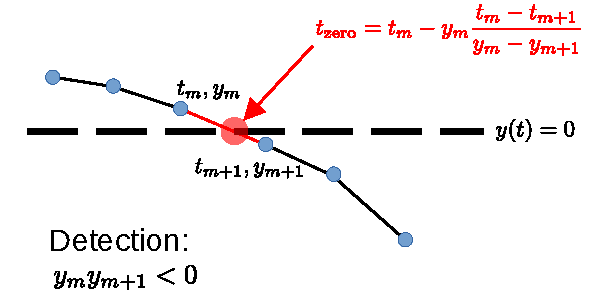
\includegraphics[width=0.65\linewidth]{diagrams/wl_zeroCross}
	\caption{Zero crossing detection in a digitally sampled interferogram, where linear interpolation of the signal is used to improve the timing of zero-crossing detection. The timing of these zero crossings entirely determines the information extracted from the interferograms in our implementation of the proposed procedure.}
	\label{fig:wlzerocross}
\end{figure}

\subsection{Interpolation}
Motivated by equation (\ref{wl_phase_slope}), we seek the phase of the test laser interferogram in terms of the reference laser interferogram phase. This can be done by interpolating the reference laser interferogram phase at the times of the test laser interferogram zero crossings. The procedure is outlined in Fig. \ref{fig:wlphaseinterpolation}.

\begin{figure}[H]
	\centering
	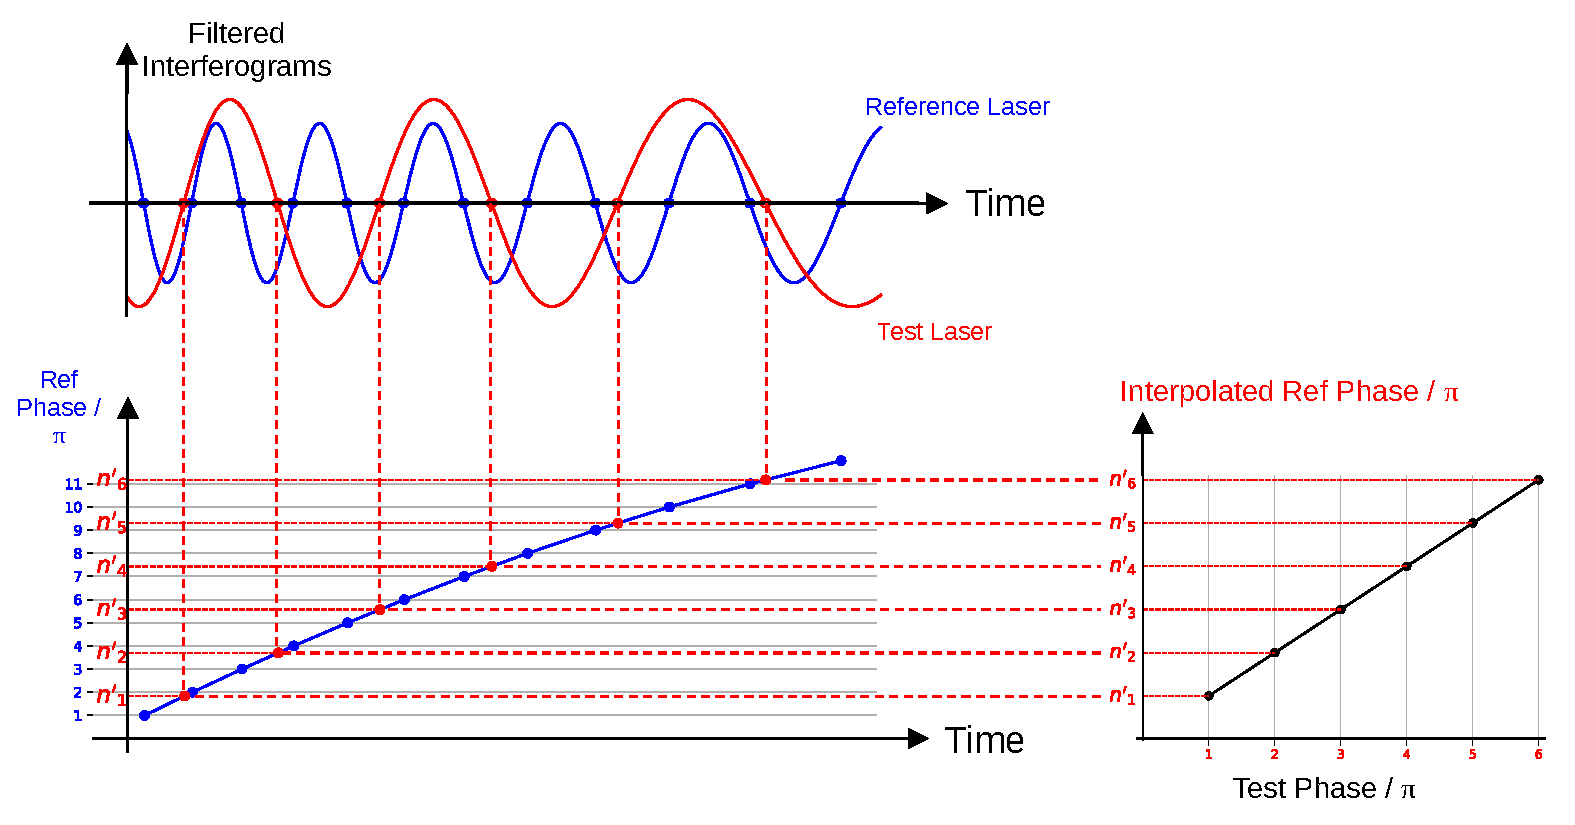
\includegraphics[width=1.0\linewidth]{diagrams/wl_phaseInterpolation}
	\caption{Diagram of procedure for the estimation of wavelength ratios optimized for digitally sampled interferograms. %The procedure does not require the storage of the entire waveform data, and can be evaluated in nearly real-time, up to the delay introduced by the interpolation stage.
	This diagram illustrates the procedure for estimating wavelength ratios optimized for digitally sampled interferograms. The blue curve in the lower left is constructed by plotting the cumulative number of reference zero-crossings against their respective timings. The timings of the test zero-crossings are then interpolated along this curve to determine $n'_j$, which represents the interpolated counting number of the $j^\mathrm{th}$ test zero-crossing. In the right pane, these values are plotted on the vertical against the test laser cumulative counting number. The slope of the resulting line gives the ratio of wavelengths.
	}
	\label{fig:wlphaseinterpolation}
\end{figure}

We can imagine this interpolation procedure pictorially by following Fig. \ref{fig:wlphaseinterpolation} as follows. We first construct a plot of the reference interferogram phase by marking the x-axis with the times of the zero crossings of the reference interferogram and the y-axis with the number of the zero crossing, incrementing by one each time a zero crossing is encountered. In the construction of Fig. \ref{fig:wlphaseinterpolation}, this is the blue plot in the lower-left pane. Then for each $i^\mathrm{th}$ zero crossing of the test laser interferogram, we interpolate this plot to find $n'_i$. As a concrete example, the value of $n'_3$ in Fig. \ref{fig:wlphaseinterpolation} is between 5 and 6.

We show explicitly this step as a linear interpolation. This interpolation step may be performed with higher order methods which consider many different points \cite{book_numerical_Press2007}, but for this application these methods seem to give little advantage over a simple linear interpolation. As depicted in Fig. \ref{fig:wllinearinterpolate}, for a zero crossing of the test laser interferogram occurring at a time $\tau_j$ between the zero crossing times $\tau^\mathrm{ref}_i$ and $\tau^\mathrm{ref}_{i+1}$ of the reference laser interferogram having numbers $n_i$ and $n_i + 1$, the interpolated zero crossing number is
\begin{equation}
	n'_j = \frac{\tau_j - \tau_i^\mathrm{ref}}{\tau_{i+1}^\mathrm{ref} - \tau_i^\mathrm{ref}} + n_i
\end{equation}

\begin{figure}[H]
	\centering
	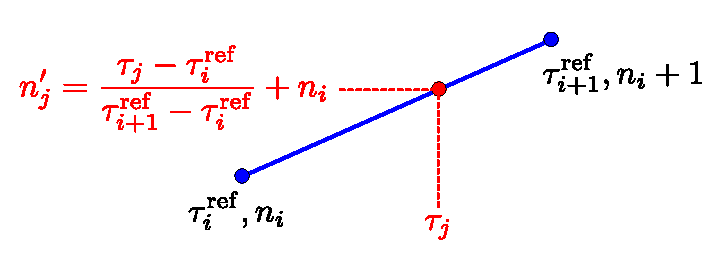
\includegraphics[width=0.5\linewidth]{diagrams/wl_linearInterpolate}
	\caption{Interpolation of the reference interferogram zero crossing times. This is depicted here as a simple linear interpolation, which is sufficient for interferogram oscillation frequencies which are far under the Nyquist value for the acquisition system. This interpolation stage determines how much of the interferogram waveform must be stored in memory at a particular time by the acquisition system.}
	\label{fig:wllinearinterpolate}
\end{figure}

\subsection{Slope Determination}
The final determination of wavelength is given by the slope of the linear fit which is made through the points in the lower-right of Fig. \ref{fig:wlphaseinterpolation}. This consists of the points \newline $(1, n'_1),\;(2, n'_2)\,\ldots\,(N, n'_N)$, where $N$ zero crossings of the test laser interferogram could be interpolated between crossings of the reference laser interferogram. The slope of the regression line is derived in the appendix and is given by equation (\ref{append_linreg_slope}), which simplifies using the known abscissa values
\begin{equation} \label{wl_wavelength_slope}
	\frac{\lambda}{\lambda_\mathrm{ref}} = 6\frac{
		(N+1)\sum_{j=1}^{N}n'_j - 2\sum_{j=1}^{N}jn'_j }{
		N(1-N^2)
	}
\end{equation}
This gives the wavelength ratio, as measured from the timing of the zero crossings of the filtered interferograms.

The analytical formulation in Eq. (\ref{wl_wavelength_slope}) allows the slope measurement to be conducted without the computational overhead of a general-purpose regression package, which would typically require the storage of all interpolated zero-crossing locations. Because this expression relies on the accumulation of weighted sums ($\sum n'_j$ and $\sum jn'_j$), the algorithm does not need to retain the history of every detected crossing in memory; instead, it only requires the storage of the current interpolated value and the running totals of these sums.

\subsection{Python Implementation of Fringe Counting Procedure}
We present a function here which computes the wavelength of a test laser from the two interferograms of the reference laser and test laser. For this, we need to know the wavelength of the reference laser. It is assumed that the two recordings have already been filtered such that their oscillations are centered on zero.

We require first a function which returns the zero crossings of a signal using the procedure depicted in Fig. \ref{fig:wlzerocross}. The zero crossings are returned as the abscissa coordinates.
\begin{singlespace}
\begin{lstlisting}[language=Python, basicstyle=\ttfamily\footnotesize]
import numpy as np

def getZeroCrossings(x, y):
    """
    Detect and interpolate the x-coordinates where the signal 'y' crosses
    zero.

    Parameters
    ----------
    x : array_like
        The independent variable (coordinates). Must be of the same length 
        as `y`.
    y : array_like
        The dependent variable (signal values) to be analyzed for zero
        crossings.

    Returns
    -------
    ndarray
        A 1D array containing the interpolated x-coordinates where the 
        signal 'y' crosses zero.

    Notes
    -----
    This function specifically detects "true" crossings (where the sign 
    actually flips). It does not explicitly handle cases where a data point 
    is exactly zero.

    Examples
    --------
    >>> x = np.array([0, 1, 2, 3, 4])
    >>> np.array([1, -1, -2, 3, 0.5])
    >>> getZeroCrossings(x, y)
    array([0.5, 2.4])
    """
    # Shift arrays to compare element i with i+1
    xi = np.array(x[0:-1])
    xi1 = np.array(x[1::])
    yi = np.array(y[0:-1])
    yi1= np.array(y[1::])

    # Identity sign changes
    mask = yi * yi1 < 0

    # Apply linear interpolation forumla to the selected indices
    xzero = -yi[mask] * (xi1[mask] - xi[mask]) /
            (yi1[mask] - yi[mask]) + xi[mask]

    return xzero
\end{lstlisting}
\end{singlespace}

The wavelength determination is then performed using the function:
\begin{singlespace}
\begin{lstlisting}[language=Python, basicstyle=\ttfamily\footnotesize]
import numpy as np
from scipy.interpolate import interp1d
from numpy import polyfit

def wavelength(ref, sig, ref_wavelength_nm=632.991):
    """
    Calculate wavelength from two sampled interferograms of CW lasers.

    Parameters
    ----------
    ref : array_like
        Reference laser interferogram, stored as 1D array.
    sig : array_like
        Test laser interferogram, stored as 1D array. 
    ref_wavelength_nm : float, optional
        The known physical wavelength of the reference signal in nanometers. 
        Defaults to 632.991 (standard HeNe laser vacuum wavelength).

    Returns
    -------
    float
        The calculated wavelength scale factor for the input signal.

    Notes
    -----
    The hardcoded value 20 is used to avoid interpolation errors, 
    and corresponds to the number of reference zero crossings ignored to 
    ensure that we have encountered a zero crossing of the test laser.
    This number is exaggerated to account for possible transient edge effects.

    """
    # Generate Artificial Time Axis
    t=np.arange(len(ref))
    
    # Zero Crossing Times
    zc_ref = zeroCrossings(t, ref)
    zc_sig = zeroCrossings(t, sig)
    
    # Enumerate Zero Crossings
    n_ref = np.arange(len(zc_ref))
    n_sig = np.arange(len(zc_sig))
    
    # Interpolation
    ref_interp = interp1d(zc_ref, n_ref)
    
    # Linear Regression
    slope = polyfit(ref_interp(zc_sig[20:-20]), n_sig[20:-20], 1)[0]
    return ref_wavelength_nm/slope
\end{lstlisting}
\end{singlespace}
Note that the hardcoded value \texttt{20} is used to avoid interpolation errors, and corresponds to the number of reference zero crossings ignored to ensure that we have encountered a zero crossing of the test laser. This number is exaggerated to account for possible transient edge effects.

\subsection{FPGA-Accelerated Acquisition Architecture}

The procedure described above can be evaluated in real time as the interferometer scans, providing a significant advantage for high-speed digital acquisition. This approach achieves the memory efficiency characteristic of simple fringe-counting methods, which compute only a ratio of total counts ($N_\mathrm{Ref}/N_\mathrm{Test}$), while providing vastly improved accuracy through the use of interpolated phase tracking and regression. By avoiding the need to store large waveform buffers, the algorithm is uniquely suited for integration into high-throughput, low-latency architectures.

In this work, the algorithm was implemented on a custom acquisition system based on a Red Pitaya single-board computer. This platform provides a high-performance environment for real-time signal processing, utilizing an on-board FPGA for high-speed data handling and a dual-channel, high-resolution ADC for the simultaneous capture of the reference and test laser interferograms. Crucially, the summation of the weighted sums is performed directly within the FPGA fabric. To prevent overflow and maintain numerical integrity during long scans, these accumulations are implemented using 128-bit integer counters (this precision remains highly configurable) synchronized to the 125 MHz ADC clock. These extended-precision integer sums are then transferred to the operating system via block memory generators, where the final conversion to floating-point representation and subsequent scaling are performed in the software layer.

\section{Python Implementation of Linear Least Squares Fitting}
For large datasets, evaluation of the pseudoinverse formula $(A^T A)^{-1}A^T \vec{b}$ used in (\ref{leastSquares}) and (\ref{append_leastSquares}) can be numerically unstable and costly if the inverse is computed directly. Moreover, the formation of $A^T A$ can lead to a matrix which is ill-conditioned, leading to large roundoff errors and unstable inversion.

In this work, we make use of the NumPy library \cite{numpy_citation}, which has become a standard tool in data analysis with the Python programming language. Modern packages such as \newline \texttt{numpy.linalg.lstsq} avoid some of the numerical instabilities of evaluating the pseudoinverse by using matrix factorization methods \cite{LAPACK}.

The following is a function for performing fitting to $x$-$y$ data of an equation having the form (\ref{append_basis_combo}), given again here
\begin{equation*}
    f(x) = c_1 f_1(x) + c_2 f_2(x) + \ldots + c_n f_n(x)
\end{equation*}
This form is a linear combination of basis functions $f_{1\ldots n}(x)$. The function given here returns the set of coefficients $c_{1\ldots n}$ which fit the above function to the data.

Within the function, the $A$ matrix entries are scaled between $[0,1]$. This ensures that the numerical scale of the pseudoinverse computation is decoupled from the scales of the resulting concentration numbers. This can help to improve accuracy of the floating point operations within the computation.

\begin{singlespace}
\begin{lstlisting}[language=Python, basicstyle=\ttfamily\footnotesize]
import numpy as np

def fitScales(data, basisFunctions, weights=None):
    """
    Perform a weighted least-squares fit of coefficients for
    a given set of basis functions.

    This function solves the linear least-squares problem: 
    min ||W * (A*c - b)||^2, where A is the matrix of basis
    functions evaluated at the provided data points.
    Transparent normalization is performed to improve
    numerical stability during the inversion process.

    Parameters
    ----------
    data : tuple of (ndarray, ndarray)
        A tuple containing:
        * data[0] (ndarray): x-coordinates/input.
        * data[1] (ndarray): y-coordinates/target.
    basisFunctions : list of callable
        A list of functions where each function `f` takes a single input 
        and returns a value (or array) corresponding to the basis 
        expansion at that point.
    weights : ndarray, optional
        An array of weights applied to the design matrix and target vector. 
        Must be broadcastable to the shape of the evaluated basis functions. 
        If None (default), all points are weighted equally.

    Returns
    -------
    ndarray
        A 1D array of fitted coefficients (the 'res' vector) scaled back 
        to the original magnitude.
    """
    # Prepare the data, apply weighting if given
    A = [f(data[0]) for f in basisFunctions]
    if(weights is not None):
        A = np.multiply(weights, A)
        b = [ np.multiply(weights, data[1]) ]
    else:
        b=[data[1]]
    A = np.transpose(A)
    b = np.transpose(b)

    # Scale A by its maximum value for numerical stability
    norm = np.max(A)
    A = A / norm

    # Peform the solution of the over-determined system
    res = np.linalg.lstsq(A, b, rcond=None)[0]

    # Return the solution, scaled to the original coordinates
    return (res / norm).flatten()
\end{lstlisting}
\end{singlespace}

Computation of the pseudoinverse matrix $M = (A^T A)^{-1}A^T$ used in (\ref{error_conc_alpha}) and (\ref{append_leastSquares}) can be performed using the following function. The pseudoinverse is constructed column-by-column by solving the least-squares problem for each unit vector.

\begin{singlespace}
\begin{lstlisting}[language=Python, basicstyle=\ttfamily\footnotesize]
def getMatrixM(x_arr, basisFunctions, weights=None):
    """
    Compute the pseudoinverse matrix (Moore-Penrose) for a given basis 
    expansion using a stabilized least-squares approach.

    The function computes the matrix $M$ such that it acts as the 
    pseudoinverse of the design matrix $A$. To ensure numerical stability, 
    the design matrix is scaled by its maximum element before computation 
    and unscaled after.

    Parameters
    ----------
    x_arr : ndarray
        The independent variable (input coordinates) at which to 
        evaluate the basis functions.
    basisFunctions : list of callable
        A list of functions where each function `f` takes a single input 
        and returns a value (or array) corresponding to the basis 
        expansion at that point.
    weights : ndarray, optional
        An array of weights applied to the design matrix rows. 
        Must be broadcastable to the shape of the evaluated basis functions. 
        If None (default), all points are weighted equally.

    Returns
    -------
    ndarray
        The pseudoinverse matrix M
    """

    A = [f(x_arr) for f in basisFunctions]
    if(weights is not None):
        A = np.multiply(weights, A)
    A = np.transpose(A)
    norm = np.max(A)
    A = A/norm

    M = []
    for i in range(A.shape[0]):
        unitVect = np.zeros(A.shape[0])
        unitVect[i] = 1.0
        res = np.linalg.lstsq(A, unitVect, rcond=None)
        M.append(res[0]/norm)
    M = np.transpose(M)
    return M
\end{lstlisting}
\end{singlespace}

The following function is a wrapper function which computes explicitly the formula (\ref{error_conc_alpha}), given the standard deviations of the absorption measurements.

\begin{singlespace}
\begin{lstlisting}[language=Python, basicstyle=\ttfamily\footnotesize]
def getFitErrors(x_arr, basisFunctions, stds, weights=None):
    """
    Calculate the propagated standard deviations of the fitted coefficients.

    Parameters
    ----------
    x_arr : ndarray
    The independent variable (input coordinates) used to evaluate 
    the basis functions.
    basisFunctions : list of callable
    A list of functions where each function `f` takes a single input 
    and returns a value/array at that point.
    stds : ndarray
    An array of standard deviations (uncertainties) corresponding to 
    each data point in the input set. Must have the same length as `x_arr`.
    weights : ndarray, optional
    An array of weights applied during the matrix computation. 
    Must be broadcastable to the shape of the evaluated basis functions.

    Returns
    -------
    ndarray
    A 1D array of size `Nr` (number of basis functions) containing 
    the propagated standard deviation for each coefficient.
    """

    # Retrieve the pseudoinverse matrix M
    M = getMatrixM(x_arr, basisFunctions, weights=weights)
    # Nr: Number of basis functions, Nc: Number of data points
    Nr, Nc = M.shape

    errs = np.zeros(Nr)

    # Propagation of error formula: sum of (weight * uncertainty)^2
    # Here M[i,j] acts as the sensitivity coefficient
    for i in range(Nr):
        for j in range(Nc):
            errs[i] = errs[i] + M[i, j]**2 * stds[j]**2

        # Take square root to convert variance back to standard deviation
        errs[i] = np.sqrt(errs[i])

    return np.array(errs)

\end{lstlisting}
\end{singlespace}

\section{Rapid Fitting of Cavity Ringdown Recordings} \label{sec:subsys_rapidLMfit}
The typical approach of determining the ringdown time of a cavity is to fit the exponentially decaying optical signal using a nonlinear fitting method. Such methods can be costly in terms of computational time and complexity, especially when implemented from a general fitting package. While methods have been presented which enable rapid ringdown time estimation \cite{crds_freq_domain, frontiers_mol_spec}, these always involve some trade-off in the accuracy of the retrieved fit. An exception can be made for recently investigated neural-network based fitting routines \cite{crds_ringdownFit_neuralNet}

In this section, we present formulas for the rapid evaluation of the Levenberg-Marquardt algorithm in the specialized case of the exponential decay model with an undermined offset. This is combined with a robust procedure for construction of an initial guess. The combination of these two optimizations gives a fitting procedure which always converges with a fixed number of iterations with few exceptions.

It is a simple matter to extract the ringdown time from a signal of the type
\begin{equation}\label{noOffsetModel}
	f(t) = A e^{-t/\tau}
\end{equation}
This can be done by fitting the slope of $\log f$ plotted against time. However, this procedure breaks down as soon as a simple DC offset is added to the signal
\begin{equation}\label{model}
	f(t) = A e^{-t/\tau} + B
\end{equation}

\subsection{Levenberg-Marquandt Algorithm for Exponential Decay with Offset}

The Levenberg-Marquandt algorithm is a nonlinear iterative algorithm for finding a set of parameters that make a model equation fit a set of data points by the least total squared residual. %In order for the algorithm to converge to a fit in a small number of steps, a good initial guess for the fit parameters is needed. Using the algorithm in section \ref{fpgaAlg}, we can come up with a set of good initial parameters that can allow the Levenberg-Marquandt algorithm to converge in a fixed number of iterations.

Let us define a model function $f(t;\; \vec{\beta} )$ containing the set of parameters given by the vector $\vec{\beta}$. For an initial guess of the parameters $\vec{\beta_0}$, we can retrieve a refined set of parameters
\begin{equation}\label{lmfit_iterationEqn}
	\vec{\beta} = \vec{\beta_0} + \vec{\delta}
\end{equation}
that is given by the gradient descent of the least squares weighting function. The change to the parameters $\vec{\delta}$ is given by solving the matrix equation
\begin{equation}\label{lmfit_matrixSolve}
	\left[ J^T J + \lambda\cdot\text{diag}\left( J^T J \right) \right] \vec{\delta} = J^T \left[\vec{y} - \vec{f}(\vec{\beta}) \right]
\end{equation}
Here $\lambda$ is a damping factor that controls speed of convergence and overshoot. The matrix $J$ is the Jacobian of the model function, defined by
\begin{equation}
	\vec{J_i} = \frac{\partial \vec{f}(t_i,\vec{\beta})}{\partial \vec{\beta}}
\end{equation}

This process is repeated until convergence is obtained. For the specific case of the model function in (\ref{model}), we have the following components for $J$

\begin{eqnarray}
	\vec{J_A} &= \frac{\partial \vec{f}}{\partial A} &= e^{-\vec{t}/\tau} \\
	\vec{J_B} &= \frac{\partial \vec{f}}{\partial B} &= \vec{1} \\
	\vec{J_\tau} &= \frac{\partial \vec{f}}{\partial \tau} &= A\frac{\vec{t}}{\tau^2}e^{-\vec{t}/\tau} 
\end{eqnarray}

Substituting these, we obtain the following for the left hand side of equation (\ref{lmfit_matrixSolve})

\begin{equation*}
	%\begin{pmatrix}
	%	\vec{J_A} \cdot \vec{J_A} & \vec{J_A} \cdot \vec{J_B} & \vec{J_A} \cdot \vec{J_\tau} \\ 
	%	\vec{J_B} \cdot \vec{J_A} & \vec{J_B} \cdot \vec{J_B} & \vec{J_B} \cdot \vec{J_\tau} \\ 
	%	\vec{J_\tau} \cdot \vec{J_A} & \vec{J_\tau} \cdot \vec{J_B} & \vec{J_\tau} \cdot \vec{J_\tau}
	%\end{pmatrix} \vec{\delta}
	%+ \lambda\cdot\text{diag}\left( J^T J \right)\vec{\delta}
	%=
	\begin{pmatrix}
		(1+\lambda)s_2 & s_1 & \frac{A}{\tau^2}s_4 \\ 
		s_1 & (1+\lambda)N & \frac{A}{\tau^2}s_3 \\ 
		\frac{A}{\tau^2} & \frac{A}{\tau^2}s_3 & \frac{A^2}{\tau^4}(1+\lambda)s_5
	\end{pmatrix} \vec{\delta}
\end{equation*}

For simplicity of notation, we have defined the following sums which can be evaluated analytically using the fact that the values of $t_n$ are known from the sampling time $t_s$ as $t_n = n t_s$. Using the definition $R \equiv e^{-t_s/\tau}$, the sums over the $N$ number of samples is carried out with $n=1\ldots N-1$
\begin{eqnarray}
	s_1 &= \sum_n e^{-t_n/\tau} &= \frac{1-R^N}{1-R} \\
	s_2 &= \sum_n e^{-2t_n/\tau} &= \frac{1-R^{2N}}{1-R^2} \\
	s_3 &= \sum_n t_n e^{-t_n/\tau} &= t_s \frac{R - N R^N + (N-1) R^{N+1}}{(1-R)^2} \\
	s_4 &= \sum_n t_n e^{-2t_n/\tau} &= t_s \frac{R^2 - NR^{2N} + (N-1) R^{2N+2}}{(1-R^2)^2} \\
	s_5 &= \sum_n t_n^2 e^{-2t_n/\tau} &= t_s^2 \frac{-R^2 - R^4 +N^2R^{2N} + (1+2N-2N^2)R^{2+2N}+(N-1)^2 R^{4+2N}}{(R^2-1)^3} \nonumber \\
\end{eqnarray}

The right hand side of equation (\ref{lmfit_matrixSolve}) can then be seen to be equal to

\begin{equation}
	\begin{pmatrix}
		\vec{J_A}^T \\ 
		\vec{J_B}^T \\ 
		\vec{J_\tau}^T
	\end{pmatrix}
	\left(\vec{y} - \vec{f}(\beta) \right) 
	=
	\begin{pmatrix}
		r_1 - A s_2 - B s_1 \\ 
		r_2 - A s_1 - B N \\ 
		\frac{A}{\tau^2}\left( r_3 -A s_4 - B S_3 \right)
	\end{pmatrix} 
\end{equation}
Here we have defined the following sums which must be evaluated on the data points.
\begin{align}
	r_1 = \sum_n y_n e^{-t_n/\tau} &&
	%r_1 = \sum_n y_n R^n &&
	r_2 = \sum_n y_n &&
	r_3 = \sum_n t_n y_n e^{-t_n/\tau}
\end{align}

In terms of these variables, the components of $\vec{\delta}$ can be solved for. We then have the explicit expressions for how the parameters $A$, $B$, and $\tau$ are updated for each iteration of the algorithm	
\begin{align}
	\delta_A &=\frac{r_1(s_3^2 -N(1+\lambda)^2 s_5) + r_2 (-s_3 s_4 + (1+\lambda) s_1 s_5) + r_3 \frac{\tau^2}{A}(-s_1 s_3 + (1+\lambda)N s_4)}{s_2(1+\lambda)\left[(1+\lambda)^2 N s_5 - s_3^2 \right] + s_1 \left[-s_1 s_5 (1+\lambda) + s_3 s_4 \right] + s_4\left[ s_1 s_3 - (1 + \lambda)N s_4\right]} \\
	\delta_B &= \frac{r_1(-s_3s_4 +(1+\lambda)s_1s_5) + r_2 (s_4^2 - (1+\lambda)^2 s_2 s_5) + r_3 \frac{\tau^2}{A}(-s_1 s_4 + (1+\lambda)s_2 s_3)}{s_2(1+\lambda)\left[(1+\lambda)^2 N s_5 - s_3^2 \right] + s_1 \left[-s_1 s_5 (1+\lambda) + s_3 s_4 \right] + s_4\left[ s_1 s_3 - (1 + \lambda)N s_4\right]} \\
	\delta_\tau &=\frac{\tau^2}{A} \frac{r_1(-s_1s_3 +(1+\lambda)Ns_4) + r_2 (-s_1s_4 + (1+\lambda)^2 s_2 s_3) + r_3 \frac{\tau^2}{A}(s_1^2 - (1+\lambda)^2N s_2)}{s_2(1+\lambda)\left[(1+\lambda)^2 N s_5 - s_3^2 \right] + s_1 \left[-s_1 s_5 (1+\lambda) + s_3 s_4 \right] + s_4\left[ s_1 s_3 - (1 + \lambda)N s_4\right]}
\end{align}

Since the $s_i$ terms can be evaluated analytically, only the $r_i$ sums need to be calculated for each iteration of the algorithm. Now we have for an initial guess for the parameters $A$, $B$, $\tau$, a solution for how these parameters should be changed to optimize the fit to the data.

\subsection{Finding an Initial Guess}
The real-time performance of the nonlinear fitting routine can be drastically improved with an initial guess which is already close to the optimized parameters. We describe here a robust method for obtaining such an initial guess. This method requires two passes through the captured data; the first pass gives an estimate of the ringdown time and can be evaluated in parallel with the data acquisition itself, while the second pass gives an estimate for the $A$ and $B$ coefficients.

\subsubsection{Ringdown time estimate}
The ringdown time can be determined from the Fourier coefficients of the captured signal in a manner similar to that which is used in \cite{crds_freq_domain}. We define the quantities $S_n$ and $C_n$ by the following Fourier integrals of the signal
\begin{align}
	S_n \equiv \int_{0}^{T}y(t) \sin \left(\frac{2\pi n t}{T}\right)\, dt
	\qquad\qquad\qquad
	C_n \equiv \int_{0}^{T}y(t) \cos \left(\frac{2\pi n t}{T}\right)\, dt
\end{align}
If the photodetector signal $y(t)$ is well modeled by the function $f(t)$, then using a simple integration by parts
\begin{equation}
	C_n = \int_0^T e^{-t/ \tau} \cos \left( \frac{2 \pi n t}{T} \right) dt
	=
	\cancel{\frac{2 \pi n}{T}  e^{-t/ \tau} \sin \left( \frac{2 \pi n t}{T} \right) \Biggr|_0^T} +
	\frac{1}{\tau} \frac{T}{2 \pi n}  \int_0^T e^{-t/ \tau} \sin \left( \frac{2 \pi n t}{T} \right) dt
\end{equation}
we see that the sine integrals $S_n$ are related to the cosine integrals $C_n$ by the relation
\begin{equation}
	\frac{S_n}{C_n} = \frac{2\pi \tau}{T} n
\end{equation}
By evaluating the ratio $S_n/C_n$ for several values of $n>0$, a straight line can be constructed by plotting the ratio $S_n/C_n$ against the harmonic number $n$. \textit{The slope of this line then gives the ringdown time} $\tau$ since the observation period $T$ is known and chosen beforehand.

For $n>0$, the $S_n$ and $C_n$ have no contribution from the DC term in the photodetector signal $B$. It is clear that this method is immune to the signal offset.

\subsubsection{Estimate of the $A$ and $B$ coefficients}
Once a guess for the ringdown time $\tau$ is obtained by the above Fourier method, the two component linear decomposition formulas in (\ref{append_lsq_two_comp}) can be directly used to obtain the scale coefficients $A$ and $B$ with the substitutions $f_1(t) = e^{-t/\tau}$ and $f_2(t) = 1$.

All three dot-product combinations of the two basis functions are easily computed analytically
\begin{align}
	a_{11} = R^2 \frac{1 - R^{2N}}{1-R^2} && a_{22} = N && a_{12} = R \frac{1 - R^N}{1 - R} &&\text{where}&& R \equiv e^{-t_s/\tau}
\end{align}
In the above expressions $t_s$ is the sampling time of the ringdown signal, which is composed of the samples $\left\{y_1\; y_2\;\ldots\; y_N\right\}$. These samples enter into the initial guess formation procedure through the sums
\begin{align}
	\bar{a}_1 = \sum_{n=1}^{N} y_n e^{-nt_s/\tau} && \bar{a}_2 = \sum_{n=1}^{N} y_n
\end{align}
Once the above quantities have been computed using our initial estimate for the ringdown time $\tau$, we can then write the initial guess for the $A$ and $B$ coefficients as
\begin{align}
	A = \frac{a_{22} \bar{a}_1 - a_{12}\bar{a}_2}{a_{11}a_{22} - a_{12}^2}
	&&
	B = \frac{a_{11} \bar{a}_2 - a_{12}\bar{a}_1}{a_{11}a_{22} - a_{12}^2}
\end{align}

The above procedure for finding the initial guess for $A$ and $B$ only requires a single parse through the data. Since we require beforehand an estimate of $\tau$, this cannot be evaluated simultaneously with the data acquisition.

%\subsection{Fitting on a Deadline -- Implementation in Real-Time Acquisition System}

\section{Implementation of the Acetone Cross Section in Computer Code} \label{sec:subsys_acetone_function}
The following function gives the fitted function describing the NIR acetone cross section. This function is plotted in Fig. \ref{fig:acetone_broadband_superfit}, and the hard-coded values used are given in Table \ref{tbl:acetone_broadband_coeffs} and Table \ref{table:acetone_coeffs}. The following code is given in the Python programming language.

\subsection{Acetone NIR Cross Section}
Reported in this section is a Python function for easily evaluating the acetone cross section model which was presented in Sec. \ref{sec:acetone_broadband} and Eq. (\ref{acetone_super_model}). The hard-coded coefficients are the fit coefficients presented in Table \ref{tbl:acetone_broadband_coeffs}. Included is a helper function \texttt{gauss(x, c[0], c[1], c[2])} which is used to evaluate a single Gaussian peak. The asymmetric peak function (\ref{sigma_tilde}), along with some of the coefficients of Table \ref{table:acetone_coeffs} are also used.

\begin{singlespace}
\begin{lstlisting}[language=Python, basicstyle=\ttfamily\footnotesize]
import numpy as np

def gauss(x, A, x0, w):
    """
    Compute the Gaussian function for a single peak.

    Parameters
    ----------
    x : ndarray
        The spectral coordinate array (wavelength in nm).
    A : float
        Amplitude of the peak.
    x0 : float
        The center position of the peak.
    w : float
        The width parameter (standard deviation/scale) of the Gaussian.
    
    Returns
    -------
    ndarray
        The evaluated Gaussian function at points x.
    """
    return A*np.exp(-(x-x0)**2/w**2)

def acetone_NIR_xs(x):
    """
    Calculate the absorption cross-section of Acetone in the NIR spectrum.

    This function computes the total absorption cross-section by summing 
    a series of Gaussian absorption lines and adding a specific 
    asymmetric feature (modeled via an arctan/Lorentzian-style term). 

    Parameters
    ----------
    x : ndarray
        The spectral coordinate array (wavelength in nm) at which to 
        evaluate the cross-section.

    Returns
    -------
    ndarray
        The calculated absorption cross-section values in units of cm^2, 
        with the same shape as the input `x`.
    """
    # Empirical constants for the asymmetric feature
    p0 = 0.70523665       # The stationary Lorentzian component (nm)
    p1 = 3.30411644e-01   # The local asymmetry of the peak
    p2 = 1672.4421        # Center of the asymmetric feature (nm)
    p3 = 3.39664499e-01   # Clamping term (nm)
    d1 =  4.07793263e-22  # Amplitude of asymmetric peak (cm^2)
    d0 = -3.61813970e-24  # Constant offset term (cm^2)

    # Gaussian peak parameters: [Amplitude, Center, Width]
    cg =  [ [1.35986073e-23, 1.60825527e+03, 1.70398884e+01],
            [1.19850011e-22, 1.65089421e+03, 1.73307837e+01],
            [7.74849891e-24, 1.65172811e+03, 4.22113059e-01],
            [3.83851582e-22, 1.66898148e+03, 2.89021701e+00],
            [2.17705109e-22, 1.66775570e+03, 5.41898839e+00],
            [2.32033931e-23, 1.67044823e+03, 5.15654864e-01],
            [6.77081682e-22, 1.67519932e+03, 5.02332894e+00],
            [5.40555517e-22, 1.68828973e+03, 5.47489581e+00],
            [2.39423927e-23, 1.69132528e+03, 5.43943755e-01],
            [2.71987962e-22, 1.69494138e+03, 4.09722699e+00],
            [5.09704537e-22, 1.70687072e+03, 2.63261427e+01],
            [7.91604650e-22, 1.73391534e+03, 1.39920104e+01],
            [9.21396457e-23, 1.75763838e+03, 5.57521753e+00],
            [3.13335887e-22, 1.77522543e+03, 1.18572793e+01],
            [2.53193043e-23, 1.84785802e+03, 7.63312916e+00],
            [1.91223143e-22, 1.93687181e+03, 1.37439004e+01] ]

    out = np.zeros_like(x)

    # Sum the Gaussian components
    for ci in cg:
        out = out + gauss(x, *ci)
    
    # Calculate the gamma term, and add the asymmetric peak
    gamma = p0 + p1*p3*np.arctan((x-p2)/p3)
    out = out + d1*gamma**2/((x-p2)**2 + gamma**2)
    
    # Return the sum, plus a constant offset
    return out + d0
\end{lstlisting}
\end{singlespace}
The above function is easily plotted using the Matplotlib library and supports vector inputs. This is shown using the following lines of Python:
\begin{singlespace}
\begin{lstlisting}[language=Python, basicstyle=\ttfamily\footnotesize]
import matplotlib.pyplot as plt

x = np.linspace(1600, 2000, 10_000)
y = acetone_NIR_xs(x)

plt.plot(x, y)

plt.xlabel("Wavelength [nm]")
plt.ylabel("Cross Section [cm$^2$]")
\end{lstlisting}
\end{singlespace}


\chapter{MATHEMATICAL DERIVATIONS}

\section{Wavelength Measurement with a Michelson Interferometer} \label{sec:wl_wavelength}
This section describes the precise measurement of wavelength ratios using the configuration of a scanning Michelson interferometer, as well as details a specialized digital algorithm designed to extract these ratios with high stability. By leveraging high-resolution phase tracking and hardware-accelerated regression, we present a method that maintains extreme precision even in the presence of non-uniform mechanical motion of the apparatus.

The basic configuration for a Michelson interferometer is shown in Fig. \ref{fig:wl_michelsonsimple}, consisting of one fixed arm having length $D$ and another movable arm having length $D + d$. Incoming light is split into two paths using a beam splitter. These two paths traverse twice the two arms of the interferometer, and are recombined using the same beam splitter onto a photodetector.
\begin{figure}[H]
	\centering
	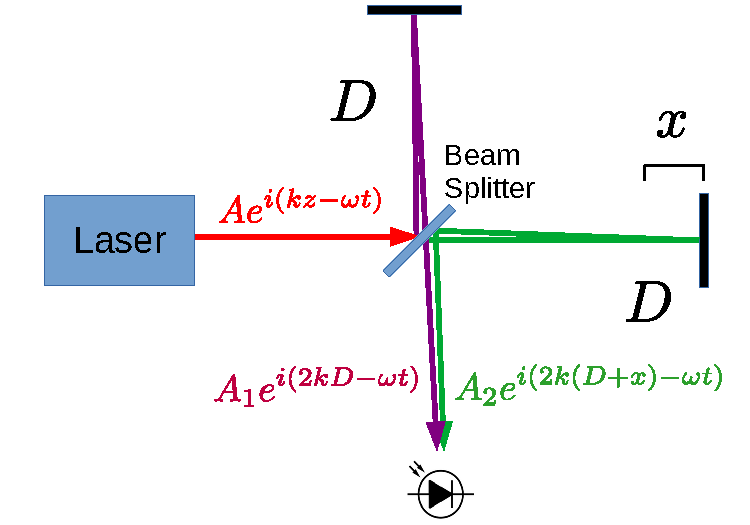
\includegraphics[width=0.5\linewidth]{diagrams/wl_michelsonSimple}
	\caption{A simplified configuration of a scanning Michelson interferometer. A beam is split into two paths (shown in green and purple) by a beam splitter. The path shown in purple traverses a distance of $2D$, while the green beam travels a length $2(D+x)$ before being recombined at the beam splitter. Due to the time varying delay between the beams, a sinusoidal pattern in time is observed on the photodetector.}
	\label{fig:wl_michelsonsimple}
\end{figure}

The incoming electric field can be described using the phasor
\begin{equation}
	E_\mathrm{in} = A e^{i(kz - \omega t)}
\end{equation}
After traversing the fixed arm for a total distance of $2D$, the contribution of light at the output of the beam splitter from this path is
\begin{equation}
	E_1 = A_1 e^{i(2kD - \omega t)}
\end{equation}
while the other path gives the contribution
\begin{equation}
	E_2 = A_2 e^{i(2k(D+x) - \omega t)} = A_2 e^{2ikx}e^{i(2kD - \omega t)}
\end{equation}
The photodetector is exposed to the sum of the two fields
\begin{align}
	E_p = E_1 + E_2 %&= A_1 e^{i(2kD - \omega t)} + A_2 e^{2ikd}e^{i(2kD - \omega t)} \\
	&= \left(A_1 + A_2 e^{2ikx}\right)e^{i(2kD - \omega t)}
\end{align}

It is clear that the field at the detector depends directly on the optical path difference (OPD) by the relation to the translation stage movement $\delta = 2x$ which is particular to the mechanical configuration of the delay. Proceeding forward, we use the OPD $\delta$ as it is independent of the particular mechanical configuration of the interferometer used to create the delay. The photodetector does not respond to the rapidly oscillating electric field, but to the time-averaged intensity, so the signal from the photodetector is proportional to
\begin{align}
	I_p(\delta) = E_p^*E_p &= \left(A_1 + A_2 e^{ik\delta}\right)\left(A_1^* + A_2^* e^{-ik\delta}\right) \\
	&= \left|A_1\right|^2 + \left|A_2\right|^2 + A_1A_2^*e^{-ik\delta} + A_1^*A_2e^{ik\delta}
\end{align}
The coefficients $A_{1,2}$ are in general complex and when written in the polar form $A_{1,2} = \left|A_{1,2}\right| e^{i\phi_{1,2}}$ the $\phi_{1,2}$ represent a constant phase shift of the output fields relative to the input field. Dropping the absolute value and writing the phase shift explicitly, the light intensity at the detector becomes
\begin{equation}\label{wl_sig_monochromatic}
	I_p(\delta) = A_1^2 + A_2^2 + A_1A_2\cos(k\delta + \phi_2 - \phi_1)
\end{equation}
The intensity detected by the photodetector is an offset sinusoidal function of the OPD $\delta$. The amplitude of this sinusoid is maximized when the beams emerging from each arm have the same field strength (or equivalently the same intensity) which occurs when $A_1 = A_2$.

\section{The Beer-Lambert law}
When light propagates through an opaque medium, some of the light is absorbed and the transmitted intensity is lowered. For now we will assume the light is monochromatic, but we can later relax this assumption using the superposition principle.

Consider a simple absorbing medium which is thin and has small completely opaque centers distributed throughout. It is clear that the change in light intensity $\Delta I$ which would be observed on the other side is proportional to the incident intensity $I$, since the transmitted intensity only consists of the locations where a "shadow" is not cast into the beam.

\begin{figure}[H]
	\centering
	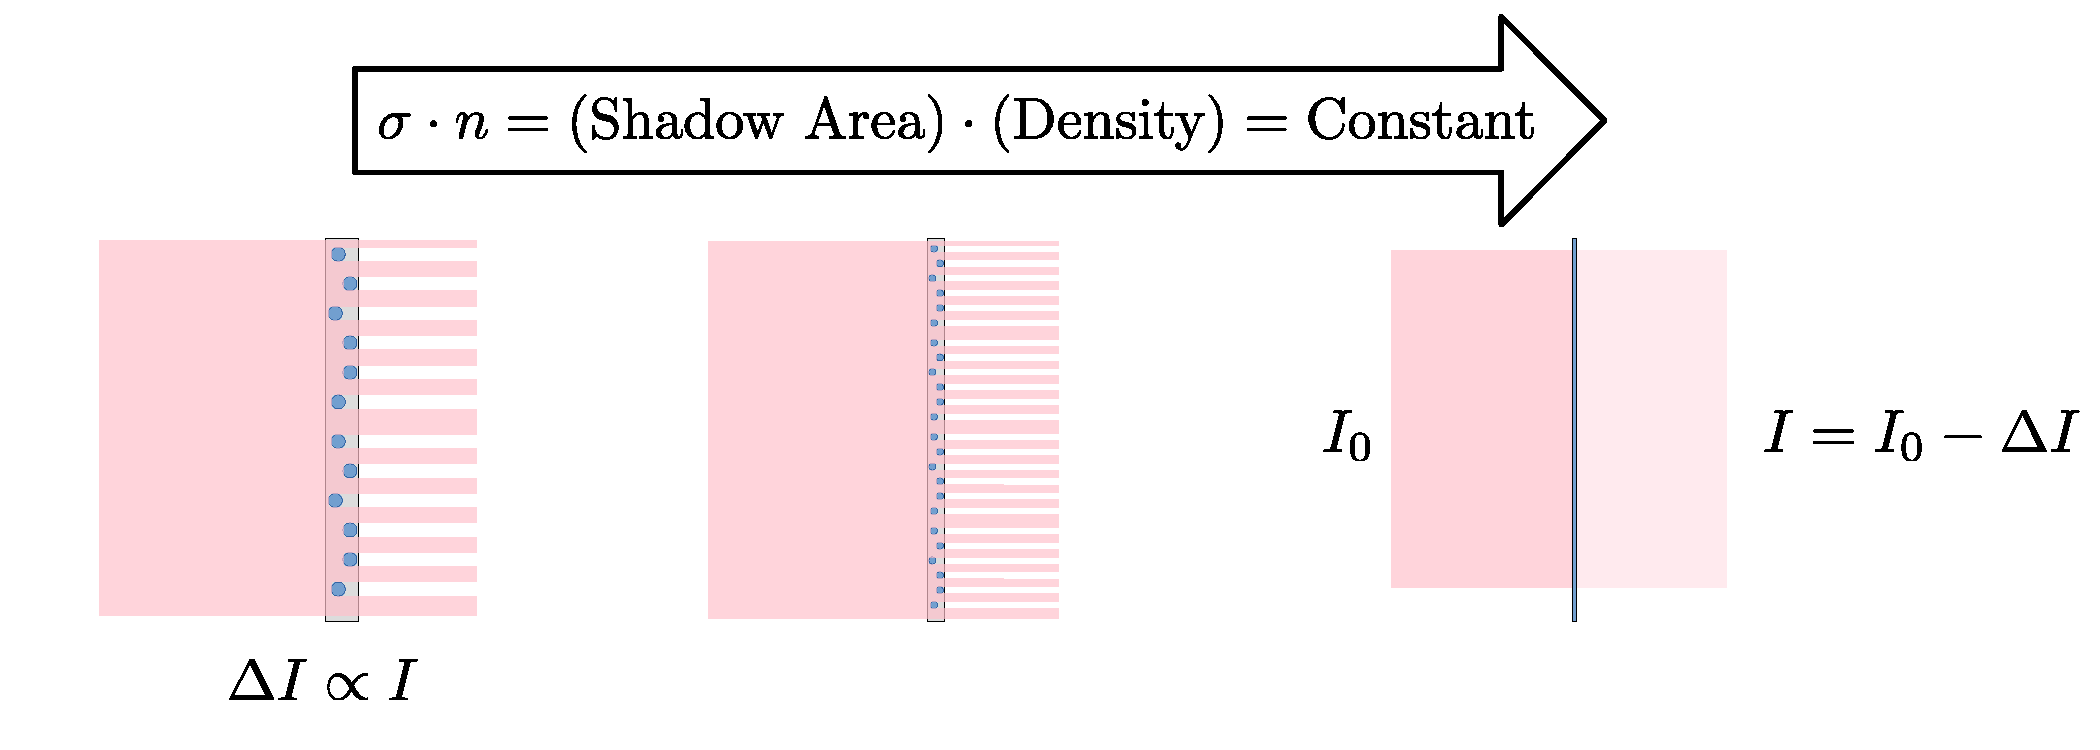
\includegraphics[width=0.9\linewidth]{diagrams/absorption_prop}
	\caption{Characterizing a material with a model of small opaque absorbing centers. The light transmitted through the material is the light that is not blocked by these objects. The change in light intensity $\Delta I$ is therefore proportional to the incident light intensity $I_0$. Depicted is the limiting process of scaling down the cross sectional area while increasing the particle density. If the same change in light intensity $\Delta I$ is to remain constant, then the product of the cross sectional area of the absorbing particles and their density must remain constant as we proceed to a thin slab.}
	\label{fig:absorption_prop}
\end{figure}

We make the assumption that thin slabs of absorbing material act independently in the sense that the change in intensity through each slab only depends on the incident intensity $\Delta I \propto I$. This would not be the case for the exaggerated case depicted in the left of Fig. \ref{fig:absorption_prop} since if an identical slab was placed in the transmitted beam path then the shadow cast by the first absorbing centers would coincide with the locations of the centers in the second slab. If we assume that these centers are randomly and homogenously distributed throughout the medium then this dependence is removed. Additionally due to the wave nature of light, the effect of coinciding shadows would be reduced by diffraction.

We can see from Fig. \ref{fig:absorption_prop} that if we shrink these small absorbing centers as we shrink the width of the slab, then there is a decreasing probability of overlapping shadows with a subsequent slab. In the limit of small scattering centers and a homogeneous distribution, the thin slabs of absorbing material behave independently of each other.

For a medium of thickness $L$, we can subdivide this length into $N$ small slices of thickness $\Delta x = L/N$ as in Fig. \ref{fig:absorption_slabs}. For a thin slice, we can presume that the change in light intensity $\Delta I$ transmitted through a small slice is proportional to the incident light intensity and the thickness of the slab. The constant of proportionality $\alpha$ characterizes the interaction of the material with the particular wavelength of light.

\begin{equation}\label{_beerDiff}
	\Delta I = - \alpha I \Delta x
\end{equation}

\begin{figure}[H]
	\centering
	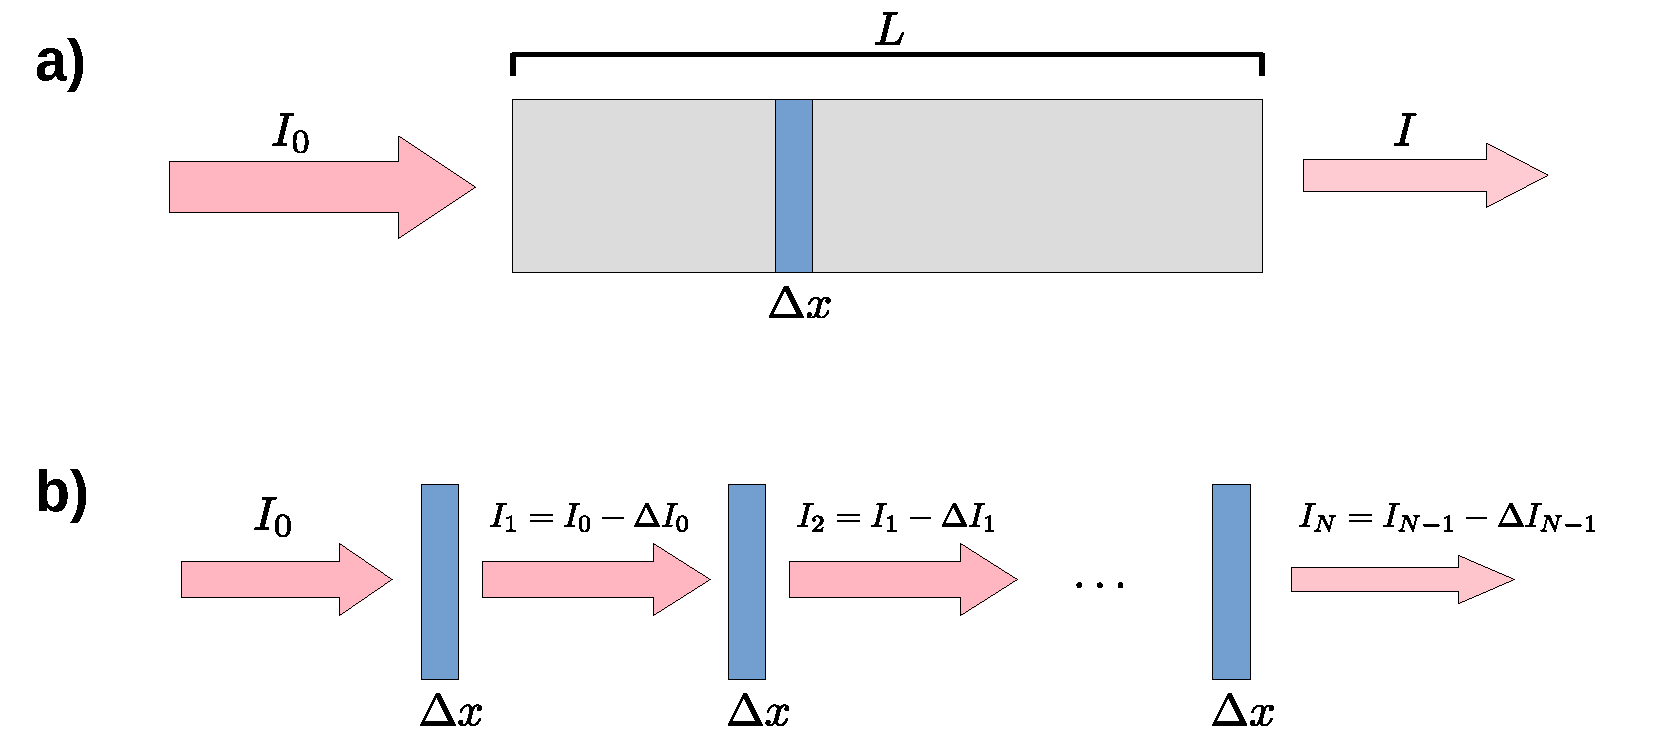
\includegraphics[width=0.7\linewidth]{diagrams/absorption_slabs}
	\caption{The construction of a finite-length absorbing material from many thin slabs. If the material of length $L$ shown in \textbf{a)} is subdivided into slabs of thickness $\Delta x$, then we have a number $N=L/\Delta x$ of such slabs. The Lambert-Beer law is obtained in the limit of the beam traversing infinitely many such absorbing slabs, as shown in \textbf{b)} for $N$ slabs.}
	\label{fig:absorption_slabs}
\end{figure}

After the first slab, the transmitted intensity $I_1$ is
\begin{align}
	I_1 &= I_0 + \Delta I_0 = I_0 \left(1 - \alpha \Delta x\right)
\end{align}
The transmitted intensity after the second slab is $I_2$ given by
\begin{align}
	I_2 &= I_1 + \Delta I_1 = I_1 \left(1 - \alpha \Delta x\right) = I_0 \left(1 - \alpha \Delta x\right)^2
\end{align}
After $N$ slabs, we have traversed the entire medium of thickness $L$. This gives the slice thickness as $\Delta x = L/N$. In terms of the incident intensity $I_0$, this is
\begin{align}
	I_N &= I_0 \left(1 - \alpha \frac{L}{N}\right)^N
\end{align}
In the limit of $N\rightarrow \infty$ slabs, this becomes
\begin{equation}
	I = \lim\limits_{N\rightarrow\infty} I_0 \left(1 - \frac{\alpha L}{N}\right)^N
\end{equation}
Evaluating this limit gives rise to the exponential function, and we arrive at the \textbf{Beer-Lambert law}
\begin{equation} \label{beer-lambert-law}
	I = I_0 e^{-\alpha L}
\end{equation}
This can also be found from (\ref{_beerDiff}) by setting $\Delta I \rightarrow dI$ and $\Delta x \rightarrow dx$ giving a differential equation, and the solution to this differential equation gives the above relation.

Since the value of $\alpha$ at the measurement wavelength is a microscopic property of the absorbing material, measurement of this value yields some information about the material. For a given material that is a solid or liquid, the density of absorbing particles is within a somewhat narrow range and a value of $\alpha$ is sufficient to characterize the optical absorption. For a gas, however, the density of absorbing particles can vary over many orders since the density of the gas varies with temperature and pressure.

In the limiting process depicted in Fig. \ref{fig:absorption_prop}, as the particle cross sectional area is scaled down, the density of particles must be scaled up by the same factor to maintain the same optical extinction. In characterizing the absorption process by opaque scattering objects, the amount of light extinction by each object is characterized by a cross section $\sigma$. If the density of opaque objects is $n$, the limiting process therefore preserves the product $n \sigma = \mathrm{const}$. This leads us to the definition of the optical cross section $\sigma$ through the relation
\begin{equation} \label{alpha_n_sigma}
	\alpha = n \sigma
\end{equation}

\subsection{Absorption Spectrum}
In general the absorption coefficient in (\ref{beer-lambert-law}) is dependent on the wavelength of light that is used for the measurement. A plot of $\alpha(\lambda)$ against the wavelength of light $\lambda$ will be referred to as an absorption spectrum. The absorption spectrum $\alpha(\lambda)$ can be extracted from a measurement of the incident and transmitted spectra, as well as the optical path length through the absorbing material by
\begin{equation}\label{beer_absorp}
	\alpha(\lambda) = -\frac{1}{L}\ln \frac{I(\lambda)}{I_0(\lambda)}
\end{equation}



In this dissertation, we will mostly be concerned with the absorption spectra of gases. For a gas, the absorption coefficient should depend on the density of particles present in the beam path. If we denote the number density as $n$, then the absorption coefficient should be proportional to this density.
\begin{equation}
	\alpha(\lambda) = n \sigma(\lambda)
\end{equation}
The $\sigma$ is referred to as the optical cross section and has units of area.

\subsection{Absorption Coefficient of a Gas Mixture}

\begin{figure}[H]
	\centering
	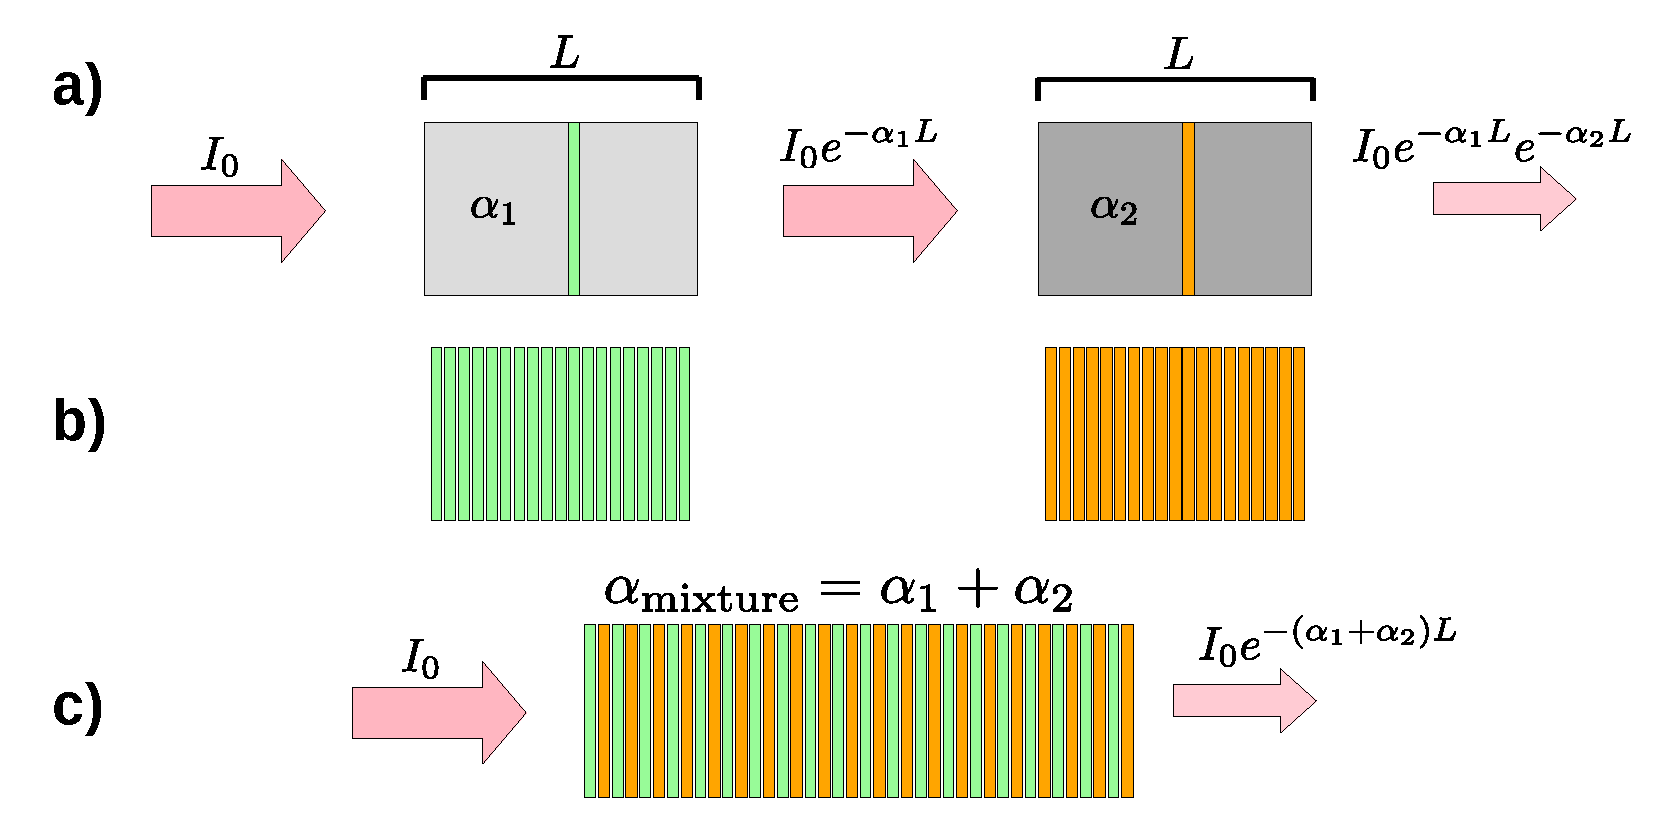
\includegraphics[width=0.7\linewidth]{diagrams/absorption_mixture}
	\caption{Using the thin slab approximation used earlier, a mixture of two gasses is depicted as alternating slabs of the two gas species. As long as the two absorption coefficients $\alpha_1$ and $\alpha_2$ are not affected by the presence of the other gas species, then this gives the same absorption as the beam passing through each pure gas separately.}
	\label{fig:absorptionmixture}
\end{figure}

For a gas mixture having several components, the absorption coefficient is a sum of the absorption coefficients of the individual components
\begin{equation}
	\alpha(\lambda) = \sum_j n_j \sigma_j(\lambda)
\end{equation}
If the mixture behaves as an ideal gas then the total number density is given by the ideal gas law in terms of the total pressure $P$ and temperature $T$
\begin{equation}
	n = \frac{P}{k_b T}
\end{equation}
and the number density of an individual species is given in terms of the partial pressure $p_j$ of that species
\begin{equation}
	n_j = \frac{p_j}{k_b T}
\end{equation}
We define the concentration $c_j$ of an individual species by mole fraction of that species, which for an ideal gas mixture is equivalent to the ratio of the partial pressure of that species to the total pressure. That is $c_j = p_j/P$. We can then write for the absorption coefficient
\begin{align}
	\alpha(\lambda) &= n_1 \sigma_1(\lambda) \;\; + \;\; n_2 \sigma_2(\lambda) \;\; + \;\; \ldots \nonumber \\
	&= \frac{p_1}{k_b T} \sigma_1(\lambda) + \frac{p_1}{k_b T} \sigma_2(\lambda) + \ldots \nonumber \\
	&= \frac{P}{k_b T} \left[\left(\frac{p_1}{P}\right)\sigma_1(\lambda) + \left(\frac{p_1}{P}\right) \sigma_2(\lambda) + \ldots \right] \nonumber\\
	&=\frac{P}{k_b T} \left[c_1\sigma_1(\lambda) + c_2 \sigma_2(\lambda) + \ldots \right]
\end{align}
In terms of the molar concentrations $c_j$, the absorption coefficient is
\begin{equation}\label{alpha_mixture}
	\alpha(\lambda) = \frac{P}{k_b T} \sum_j c_j\sigma_j(\lambda)
\end{equation}
In general the absorption cross section is dependent on the temperature, pressure, and even presence of other gas species. If the cross sections of all species contributing to an absorption signal are known, it then becomes possible to measure the concentrations of the species from an absorption spectrum. This is usually done by fitting an experimentally measured recording of absorption versus wavelength using a model absorption such as (\ref{alpha_mixture}) by finding the concentrations $c_j$ which best reproduce the data.

\section{Linear Least Squares} \label{sec:append_linear_lsq}
Suppose we have $N$ measurements $\{y_1, y_2, \ldots , y_N\}$ taken with parameters $\{x_1, x_2, \ldots , x_N\}$. We then wish to minimize the error to the function
\begin{equation} \label{append_basis_combo}
	f(x) = c_1 f_1(x) + c_2 f_2(x) + \ldots + c_n f_n(x)
\end{equation}
by an appropriate choice of $\{c_1, c_2, \ldots, c_n\}$. That is, we wish to satisfy ``as close as possible'' the equations
\begin{equation}
	y_i = c_1 f_1(x_i) + c_2 f_2(x_i) + \ldots + c_n f_n(x_i)
\end{equation}
for all $N$ sets of measurements. We can write this as an overdetermined $(N>n)$ set of linear equations
\begin{equation} \label{append_lsq_matrix_setup}
	\begin{pmatrix}
		y_1 \\
		y_2 \\
		y_3 \\
		\vdots \\
		y_N
	\end{pmatrix} =
	\begin{pmatrix}
		f_1(x_1) & f_2(x_1) & \ldots & f_n(x_1) \\
		f_1(x_2) & f_2(x_2) & \ldots & f_n(x_2) \\
		f_1(x_3) & f_2(x_3) & \ldots & f_n(x_3) \\
		\vdots & \vdots& \vdots \\
		f_1(x_N) & f_2(x_N) & \ldots & f_n(x_N)
	\end{pmatrix}
	\begin{pmatrix}
		c_1 \\
		c_2 \\
		\vdots \\
		c_n 
	\end{pmatrix}
\end{equation}	
We can write this as
\begin{equation}
	A\vec{c} = \vec{b}
\end{equation}
The least squares solution is acquired by multiplying $A^T$ on both sides to get the \textit{normal equation}
\begin{equation} \label{append_normal_equation}
	A^T A \vec{c} = A^T \vec{b}
\end{equation}
This system can then be solved by inverting the square $A^T A$ matrix and left multiply the normal equation by this inverse to obtain the least squares solution
\begin{equation}\label{append_leastSquares}
	\boxed{\vec{c} = (A^T A)^{-1} A^T \vec{b}}
\end{equation}

\subsection{The Normal Equation -- Connection to Error Minimization}

We will show that the least squares solution (\ref{append_leastSquares}) minimizes the sum of the squared errors given by
\begin{equation}
	E = \sum_i \Big[ y_i - f(x_i) \Big]^2 = (A\vec{c} - \vec{b})^T (A\vec{c} - \vec{b})
\end{equation}
This is equivalent to minimizing by our choice in $c_1\ldots c_n$ the scalar quantity
\begin{equation} \label{append_error}
	E = \sum_i \Big[ y_i - \left( c_1 f_1(x_i) + c_2 f_2(x_i) + \ldots + c_n f_n(x_i) \right) \Big]^2
\end{equation}
We can see this by setting the derivative of $E$ with respect to each $c_{1\ldots n}$ coefficient equal to zero. We write this in the vector notation
\begin{equation}
	\frac{\partial E}{\partial \vec{c}} = \vec{0}
\end{equation}
Substituting the above definition of $E$, this is
\begin{align}
	\vec{0} = \frac{\partial E}{\partial \vec{c}} &= \frac{\partial}{\partial \vec{c}} \left[(A\vec{c} - \vec{b})^T (A\vec{c} - \vec{b})\right]
\end{align}
We write this $n$ component equation in index notation following the Einstein summation convention, where repeated indices imply summation. We write the $i^\mathrm{th}$ component of the column vector $\vec{c}$ and its transpose as $\left(\vec{c}\,\right)_i=c_i$ and $\left(c^T\right)_i = c_{0i}$. The $i^\mathrm{th}$ component of the above equation is then
\begin{align}
	%0 &= \frac{\partial E}{\partial c_{i}} \left[(A\vec{c} - \vec{b})^T_{j} (A\vec{c} - \vec{b})_{j}\right] \nonumber\\
	0 &= \frac{\partial E}{\partial c_{i}} \left[(c^T A^T - b^T)_{j} (A\vec{c} - \vec{b})_{j}\right] \nonumber\\
	&= \frac{\partial E}{\partial c_{i}} \Big[(c_{0k}A_{jk} - b_{0j}) (A_{jl}c_{l} - b_j)\Big] \nonumber\\
	&= \frac{\partial E}{\partial c_{i}} \Big[ c_{0k}A_{jk}A_{jl}c_l - c_{0k}A_{jk}b_j - b_{0j}A_{jl}c_l + b_{0j}b_j \Big] \nonumber\\
	&= \delta_{ik}A_{jk}A_{jl}c_l + c_{0k}A_{jk}A_{jl}\delta_{li} - \delta_{ik}A_{jk}b_j - b_{0j}A_{jl}\delta_{li} \nonumber\\
	&= A_{ji}A_{jk}c_k + c_{0k}A_{jk}A_{ji} - A_{ji}b_j - b_{0j}A_{ji}
\end{align}
In the last step we have substituted the dummy index $l\rightarrow k$. We can see that have the same operations written twice since $c_{0k} = c_k$ and $b_{0j}=b_j$. Coming back to vector-matrix notation, the above expression is the same as
\begin{align}
	\vec{0} = 2\left(A^T A \vec{c} - A^T \vec{b}\right)
\end{align}
This then leads us again to the normal equation
\begin{equation}
	A^T A \vec{c} = A^T \vec{b}
\end{equation}

\subsubsection{Checking the Minimum}
We can check that the solution to the normal equation above provides a true minimum of the error $E$ by computing the second derivative with respect to each coefficient $c_i$. To avoid confusion in the Einstein convention with repeated $i$ index, we write the sums explicitly
\begin{align}
	\frac{\partial^2 E}{\partial c_i^2}
	&= \frac{\partial}{\partial c_i} \Big[\sum_{j,k}A_{ji}A_{jk}c_k + \sum_{j,k}c_{0k}A_{jk}A_{ji} - \sum_{j}A_{ji}b_j - \sum_{j}b_{0j}A_{ji}\Big] \nonumber\\
	&= \sum_{j,k}A_{ji}A_{jk}\delta_{ki} + \sum_{j,k}\delta_{ik}A_{jk}A_{ji} \nonumber\\
	&= 2\sum_{j}\left(A_{ji}\right)^2 \nonumber\\
	\frac{\partial^2 E}{\partial c_i^2} &> 0
\end{align}
Since the above second derivative is positive for every $i$, we see that the solution given by the normal equation is indeed a true minimum. We therefore conclude that the least-squares solution (\ref{append_leastSquares}) gives the set of coefficient $c_i$ which minimize the error sum in (\ref{append_error}).

\subsection{Two Component Solution}
We assume that we have two function $f_{1,2}(x)$ which are to be fit to the data using the model function
\begin{equation}
	f(x) = c_1 f_1(x) + c_2 f_2(x)
\end{equation}
The $N\times 2$ matrix $A$ is then
\begin{equation}
	A =
	\begin{pmatrix}
		f_1(\vec{x}) & f_2(\vec{x})
	\end{pmatrix}
\end{equation}
We proceed to compute
\begin{equation}
	A^T A =
	%\begin{pmatrix}
	%	f_1(\vec{x})\cdot f_1(\vec{x}) & f_2(\vec{x})\cdot f_1(\vec{x}) \\
	%		f_1(\vec{x})\cdot f_2(\vec{x}) & f_2(\vec{x})\cdot f_2(\vec{x})
	%\end{pmatrix}
	%=
	\begin{pmatrix}
		\sum_i f_1(x_i)^2 & \sum_i f_1(x_i)f_2(x_i) \\
		\sum_i f_2(x_i)f_1(x_i) & \sum_i f_2(x_i)^2
	\end{pmatrix}
	\equiv
	\begin{pmatrix}
		a_{11} & a_{12} \\
		a_{12} & a_{22}
	\end{pmatrix}
\end{equation}
We can immediately invert the 2x2 matrix to give
\begin{equation}
	\left(A^T A\right)^{-1} = 
	%\frac{1}{\left(\sum_i f_1(x_i)^2\right)\left(\sum_i f_2(x_i)^2\right) - \left(\sum_i f_1(x_i)f_2(x_i)\right)^2}
	\frac{1}{a_{11} a_{22} - a_{12}^2}
	\begin{pmatrix}
		a_{22} & -a_{12} \\
		-a_{12} & a_{11}
	\end{pmatrix}
\end{equation}
We now construct the matrix
\begin{equation}
	\left(A^T A\right)^{-1} A^T = \frac{1}{a_{11} a_{22} - a_{12}^2}
	\begin{pmatrix}
		a_{22}f_1(x^T)  - a_{12}f_2(x^T) \\
		-a_{12}f_1(x^T) + a_{11}f_2(x^T)
	\end{pmatrix}
\end{equation}
The coefficients $c_{1,2}$ are then given by the two components of $\left(A^T A\right)^{-1} A^T \vec{b}$. If we define $\tilde{a}_1 \equiv \sum_i y_i f_1(x_i)$ and $\tilde{a}_2 \equiv \sum_i y_i f_2(x_i)$ then we have the following formulas for the values of the fit coefficients
\begin{align} \label{append_lsq_two_comp}
	c_1 = \frac{a_{22}\tilde{a}_1 - a_{12} \tilde{a}_2}{a_{11} a_{22} - a_{12}^2}
	&\qquad&
	c_2 = \frac{a_{11}\tilde{a}_2 - a_{12} \tilde{a}_1}{a_{11} a_{22} - a_{12}^2}
\end{align}

\subsubsection{Linear Regression Formula}
Fitting a line to a set of experimentally recorded data is a task that is often used. For this we use the two component equation with
\begin{equation}
	f(x_i) = c_1 x_i + c_0
\end{equation}
This gives for the five $a$ coefficients
\begin{align}
	a_{11} = \sum_i x_i^2 && a_{12} = \sum_i x_i && a_{22}=N && \tilde{a}_1 = \sum_i y_i x_i && \tilde{a}_2 = \sum_i y_i
\end{align}
This gives the regression formula for the slope
\begin{equation}\label{append_linreg_slope}
	c_1 = \frac{N\sum x_i y_i - \left(\sum x_i\right)\left(\sum y_i\right)}{N\sum x_i^2 - \left(\sum x_i\right)^2}
\end{equation}
and for the intercept
\begin{equation}\label{append_linreg_interc}
	c_0 = \frac{\left(\sum x_i^2\right)\left(\sum y_i\right) - \left(\sum x_i\right)\left(\sum x_i y_i\right)}{N\sum x_i^2 - \left(\sum x_i\right)^2} = \bar{y_i} - c_1 \bar{x_i}
\end{equation}




\subsection{Uncertainty in the Coefficients}

For a general nonlinear function $g(x_1, x_2, \ldots, x_n)$ of the $n$ parameters $x_i$, we can estimate the deviation $\Delta g$ of the function output given the statistically independent deviations $\Delta x_1$, $\Delta {x_2}$, $\ldots$, $\Delta {x_n}$ of the input parameters by the law of propagation of errors \cite{stats_lawOfPropagationErrs}
\begin{equation} \label{append_error_prop}
	\Delta g^2 =
	\left(\frac{\partial g}{\partial x_1}\Bigg|_{\tilde{x}_1}\right)^2 \Delta {x_1}^2 +
	\left(\frac{\partial g}{\partial x_2}\Bigg|_{\tilde{x}_2}\right)^2 \Delta {x_2}^2 + \ldots +
	\left(\frac{\partial g}{\partial x_n}\Bigg|_{\tilde{x}_n}\right)^2 \Delta {x_n}^2
\end{equation}
The $\tilde{x}_i$ in the above expression are the average values of each of the $x_i$.

We consider the case of (\ref{append_leastSquares}), where for simplicity we denonte the pseudoinverse matrix $M = \left(A^T A\right)^{-1} A^T$. The function under consideration is then linear in the measured ordinate values $\vec{b}$
\begin{equation} \label{append_error_ci}
	c_i = \sum_{j} M_{ij}b_j
\end{equation}
From the law of propagation of errors (\ref{append_error_prop}), we have that the deviation of the concentration of the $i^\mathrm{th}$ coefficient is
\begin{equation}
	\Delta {c_i}^2 = \sum_{k} \left(\frac{\partial c_i}{\partial b_k}\Bigg|_{\tilde{b}_k}\right)^2 \Delta {b_k}^2
\end{equation}
From (\ref{append_error_ci}) we can evaluate the partial derivative in the above expression. There is no dependence of the matrix $M$ on the measured ordinate values $\partial M / \partial b_k = 0$, since $M$ is calculated from the functional dependences of the $f_{1\ldots n}(x)$ basis set used. With the trivial action of the partial derivative on the linear terms $\partial b_j / \partial b_k = \delta_{jk}$ we have
\begin{equation}
	\frac{\partial c_i}{\partial b_k}\Bigg|_{\tilde{b}_k} = \sum_j M_{ij} \delta_{jk} = M_{ik}
\end{equation}
We then have the deviation of the $i^\mathrm{th}$ coefficient as
%\label{error_conc_alpha} !!!!!
\begin{equation} \label{append_leastSq_error}
	\boxed{\Delta {c_i} = \sqrt{\sum_j \left(M_{ij} \, \Delta {b_j}\right)^2}}
\end{equation}

%That is, the fluctuation in the concentration is calculated in terms of the fluctuation in the measured absorption. It is now clear that measurements of the absorption coefficient which are homoscedastic, where the uncertainties of all measurements is a constant $\Delta x_i = \Delta x$, then the precision of the concentration determination scales linearly with the precision of absorption coefficient determination $\Delta c_i \propto \Delta x$.

\subsubsection{Single Basis Function Scale Uncertainty}
We consider here the specialized case of just a single basis function
$$f(x) = c_1 f_1(x)$$
The matrix then $A$ becomes that of a single column vector $\vec{f_1}$ defined as $\left(\vec{f}_1\right)_i \equiv f_1(x_i)$. It is clear in this case that $A^T A$ is just a scalar, and the matrix $M = \left(A^T A\right)^{-1} A^T$ is then just the row vector
\begin{equation}
	M = \frac{A^T}{\vec{A}\cdot \vec{A}} = \frac{f_1^T}{\vec{f_1}\cdot\vec{f_1}}
\end{equation}
Using that $M=M_{0j}$, we have from (\ref{append_leastSq_error}) the basis function scale uncertainty
\begin{equation}\label{append_error_one_general}
	\Delta c = \frac{1}{\vec{f}_1\cdot\vec{f}_1} \sqrt{\sum_j \Big(f_1(\lambda_j) \, \Delta b_j\Big)^2}
\end{equation}

For measurements that are homoscedastic, or have constant uncertainty, $\Delta b_i \equiv \Delta b$, this relation simplifies to
\begin{equation}
	\boxed{\Delta c = \frac{\Delta b}{\left|\vec{f}_1\right|}}
\end{equation}
If all of the $N$ measurements are conducted at a single input value $x_i = \tilde{x}$ where the basis function has the value $f_1 = f(\tilde{x})$, then this gives the same effect as averaging those measurements
\begin{equation}
	\boxed{\Delta c_\mathrm{avg} = \frac{\Delta b}{\sqrt{N} f_1}}
\end{equation}
For measurements all corresponding to the same $x$ value, we see that \textit{there is no difference between averaging the measured values or entering them each as separate measurements into (\ref{append_lsq_matrix_setup})}.	


\subsubsection{Coefficient Uncertainty for Two Basis Functions}
For a function given by the linear combination of two basis functions \newline $f(x) = c_1 f_1(x) + c_2 f_2(x)$, then we have the generally overdetermined $(N>2)$ system
\begin{equation*}
	\underbrace{\begin{pmatrix}
			b_1 \\
			b_2 \\
			b_3 \\
			\vdots \\
			b_N
	\end{pmatrix}}_{\begin{matrix}\vec{b}\end{matrix}} =
	\underbrace{\begin{pmatrix}
			f_1(x_1) &  f_2(x_1) \\
			f_1(x_2) &  f_2(x_2) \\
			f_1(x_3) &  f_2(x_3) \\
			\vdots & \vdots \\
			f_1(\lambda_N) & f_2(x_N)
	\end{pmatrix}}_{\begin{matrix}A\end{matrix}}
	\begin{pmatrix}
		b_1 \\
		b_2
	\end{pmatrix}
\end{equation*}
We define the corresponding vectors $\vec{f}_1$ and $\vec{f}_2$ having entries $\left(\vec{f}_{1,2}\right)_i = f_{1,2}(x_i)$ corresponding to the evaluations of each function at the measurement values $x_i$. We then have the matrices
\begin{align}
	A =
	\begin{pmatrix}
		\vec{f}_1 & \vec{f}_2
	\end{pmatrix}
	&&
	A^T =
	\begin{pmatrix}
		f_1^T \\ f_2^T
	\end{pmatrix}
	&&
	A^T A =
	\begin{pmatrix}
		\vec{f}_1 \cdot \vec{f}_1 & \vec{f}_1 \cdot \vec{f}_2 \\
		\vec{f}_2 \cdot \vec{f}_1 & \vec{f}_2 \cdot \vec{f}_2
	\end{pmatrix}
\end{align}
We see that the matrix $A^T A$ is of dimension 2x2 having entries corresponding to the scalar products of the $\vec{f}_{1,2}$ vectors. For a general 2x2 matrix having nonzero determinant, we have the inverse
\begin{equation*}
	\begin{pmatrix}
		a & b \\ c & d
	\end{pmatrix} ^ {-1}
	=
	\frac{1}{ad - bc}
	\begin{pmatrix}
		d & -b \\ -c & a
	\end{pmatrix}
\end{equation*}
In constructing the $M$ matrix, we require the inverse
\begin{equation}
	\left(A^T A\right)^{-1} = \frac{1}{f_1^2 f_2^2 - \left(\vec{f}_1\cdot\vec{f}_2\right)^2}
	\begin{pmatrix}
		f_2^2 & -\vec{f}_1\cdot\vec{f}_2 \\
		-\vec{f}_1\cdot\vec{f}_2 & f_1^2
	\end{pmatrix}
\end{equation}
Right-multiplying the above expression by $A^T$ gives the $M$ matrix
%	\begin{equation}
	%		M = \frac{k_\mathrm{B} T / P}{f_1^2 f_2^2 - \left(\vec{f}_1\cdot\vec{f}_2\right)^2}
	%		\begin{pmatrix}
		%			\;\;\;
		%			f_2^2 f_1^T - \left(\vec{f}_1 \cdot \vec{f}_2\right)f_2^T \\\\
		%			-\left(\vec{f}_1 \cdot \vec{f}_2\right)f_1^T + f_1^2 f_2^T
		%		\end{pmatrix}
	%	\end{equation}
\begin{equation}
	M = \frac{1}{f_1^2 f_2^2 - \left(\vec{f}_1\cdot\vec{f}_2\right)^2}
	\left[
	\begin{pmatrix} f_2^2 \\ -\vec{f}_1 \cdot \vec{f}_2 \end{pmatrix} f_1^T +
	\begin{pmatrix} -\vec{f}_1 \cdot \vec{f}_2 \\ f_1^2 \end{pmatrix} f_2^T
	\right]
\end{equation}
We define the overlap parameter $\gamma$ which measures the cosine of the angle between the \newline $\vec{f}_1$ and $\vec{f}_2$ vectors
\begin{equation}
	\gamma \equiv \frac{\vec f_1\cdot\vec f_2}{f_1f_2}
\end{equation}
This parameter ranges from $\pm 1$, where a value of $\left|\gamma\right| = 1$ means that $f_1$ and $f_2$ are identical up to a scale factor. In terms of the overlap parameter, the $M$ matrix is
\begin{equation}
	M = \frac{1}{1 - \gamma^2}
	\left[
	\begin{pmatrix} 1/f_1^2 \\ -\gamma/f_1f_2 \end{pmatrix} f_1^T +
	\begin{pmatrix} -\gamma/f_1f_2 \\ 1/f_2^2 \end{pmatrix} f_2^T
	\right]
\end{equation}
From (\ref{append_leastSq_error}) the errors in the coefficient estimates are
%	\begin{equation} \label{error_two_general}
	%		\begin{pmatrix}
		%			\Delta c_1 \\ \Delta c_2
		%		\end{pmatrix} = 
	%		\frac{k_\mathrm{B} T / P}{f_1^2 f_2^2 - \left(\vec{f}_1 \cdot \vec{f}_2\right)^2}
	%		\begin{pmatrix}
		%			\sqrt{\sum_i \Delta x_i\Big( f_2^2 f_{1,i} - (\vec f_1\cdot\vec f_2)f_{2,i} \Big)^2} \\ \\
		%			\sqrt{\sum_i \Delta x_i\Big( f_1^2 f_{2,i} - (\vec f_1\cdot\vec f_2)f_{1,i} \Big)^2}
		%		\end{pmatrix}
	%	\end{equation}
\begin{equation} \label{append_error_two_general}
	\begin{pmatrix}
		\Delta c_1 \\ \Delta c_2
	\end{pmatrix} = 
	\frac{1}{1 - \gamma^2}
	\begin{pmatrix}
		\sqrt{\sum_i \Delta b_i\left( \frac{1}{f_1^2}f_{1,i} - \frac{\gamma}{f_1f_2}f_{2,i} \right)^2} \\ \\
		\sqrt{\sum_i \Delta b_i\left( \frac{1}{f_2^2}f_{2,i} - \frac{\gamma}{f_1f_2}f_{1,i} \right)^2}
	\end{pmatrix}
\end{equation}
For $\gamma = 0$, corresponding to completely orthogonal $\vec{f}_1$ and $\vec{f}_2$, this gives the equivalent of (\ref{append_error_one_general}) for two independent detections when there is zero overlap between the basis functions
\begin{equation}
	\Delta c_{i} \approxeq \frac{1}{f_{i}^2} \sqrt{\sum_j \left(f_{i,j}\, \Delta b_j\right)}
\end{equation}

For measurements having constant uncertainty $\Delta  b_i = \Delta  b$, we can expand each term in the sums in equation (\ref{append_error_two_general}). For the first row, we have
\begin{equation}
	\sum_i\left(\frac{1}{f_1^2}f_{1,i} - \frac{\gamma}{f_1f_2}f_{2,i}\right)^2 = \sum_i\left(\frac{f_{1,i}^2}{f_1^4} + \frac{\gamma^2f_{2,i}^2}{f_1^2f_2^2} - 2\frac{\gamma}{f_1^3f_2}f_{1,i}f_{2,i}\right) = \frac{1}{f_1^2} - \frac{\gamma^2}{f_1^2}
\end{equation}
The second row is given simply by interchanging the $1$ and $2$ subscripts in the basis functions. In the last step we have used that $\sum_i f_{1,i}^2 = f_1^2$ and $\sum_i f_{1,i}f_{2,i} = f_1f_2\gamma$. For the case of constant measurement uncertainty, equation (\ref{append_error_two_general}) then simplifies to
\begin{equation}\label{append_error_two_constUnc}
	\boxed{\Delta c_i = 
		\frac{\Delta  b}{\left|\vec f_i\right| }
		\frac{1}{\sqrt{1 - \gamma^2}}}
\end{equation}

\subsubsection{Unresolved Baseline}
Using as $f_2(\lambda) = 1$, the corresponding vector, magnitude and overlap parameter are
\begin{eqnarray}
	\vec{f}_2 = \vec{1} &\qquad
	f_2 ^2 = N &\qquad
	\gamma = \frac{\vec{f}_1 \cdot \vec{f}_2}{\left|\vec f_1\right|\sqrt{N}} = \frac{1}{\sqrt{N}\left|\vec f_1\right|}\sum_i f_{1,i} \equiv \frac{f_\mathrm{Avg}}{f_\mathrm{RMS}}
\end{eqnarray}
Above we have defined the average function value $f_\mathrm{Avg} \equiv \frac{1}{N}\sum_i f_{1,i}$ and the root-mean-square value $f_\mathrm{RMS} \equiv \sqrt{\frac{1}{N}\sum_i f_{1,i}^2} = \left|\vec f_1\right|/\sqrt{N}$.
The uncertainty of the coefficients are then
\begin{align}
	\Delta c &= \frac{\Delta b}{\sqrt{N}}\frac{1}{\sqrt{f_\mathrm{RMS}^2 - f_\mathrm{Avg}^2}} \\\nonumber\\
	\Delta B &= \frac{\Delta b}{\sqrt{N}}\frac{1}{\sqrt{1 - f_\mathrm{Avg}^2/f_\mathrm{RMS}^2}}
\end{align}

\subsubsection{General Basis}
\begin{align}
	A = 
	\begin{pmatrix}
		\vec{f}_1 & \vec{f}_2 & \ldots & \vec f_m
	\end{pmatrix}
	&&
	A^T =
	\begin{pmatrix}
		f_1^T \\ f_2^T \\ \vdots \\ f_m^T
	\end{pmatrix}
	&&
	A^T A = 
	\begin{pmatrix}
		\vec{f}_1 \cdot \vec{f}_1 & \vec{f}_1 \cdot \vec{f}_2 & \ldots & \vec f_1\cdot\vec f_m \\
		\vec{f}_2 \cdot \vec{f}_1 & \vec{f}_2 \cdot \vec{f}_2 & \ldots & \vec{f}_2 \cdot \vec{f}_m \\
		\vdots & \vdots\ & \ddots & \vdots \\
		\vec{f}_m \cdot \vec{f}_1 & \vec{f}_m \cdot \vec{f}_2 & \ldots & \vec f_m\cdot\vec f_m
	\end{pmatrix}
\end{align}
The element in the $i^\mathrm{th}$ row and $j^\mathrm{th}$ column of the $A^TA$ matrix is
\begin{equation}
	B_{ij} \equiv \left(A^TA\right)_{ij} = \vec f_i\cdot\vec f_j
\end{equation}
The inverse of this matrix is written in terms of the minors $M_{ij}$
\begin{equation}
	\left(B^{-1}\right)_{ij} = \frac{(-1)^{i+j}M_{ij}}{\det\left(B\right)}
\end{equation}
Using the Levi-Civita symbols, we write this as
\begin{equation}
	\left(B^{-1}\right)_{ij} = \frac{1}{(n-1)!\det\left(B\right)}\epsilon_{i i_2\ldots i_n}\epsilon_{j j_2\ldots j_n}B_{i_2j_2}B_{i_3j_3}\ldots B_{i_nj_n}
\end{equation}

\section{Series Derivation of CRDS Weight Function} \label{sec:append_weight_series_crds}

%For this discussion we will drop the dependence on wavelength of the baseline ring-down time $\tau_0(\lambda) \rightarrow \tau_0$ and assume it is constant. 

Under the non-interacting gas approximation discussed in Sec. \ref{chap:fitting_spectra}, the model absorption of a gas mixture is simply a linear combination of known absorption cross section functions
\begin{equation}
	\alpha_\mathrm{m}(\lambda) = a_1 \sigma_1 (\lambda) + \ldots + a_n \sigma_n(\lambda)
\end{equation}
having unknown proportional coefficients. These proportional coefficients are determined by setting up the over-determined system given by (\ref{fit_spectrum})
and then the least-squares solution to the above system is given at once by (\ref{leastSquares}), or equivalently (\ref{append_leastSquares}). In the case of Cavity Ringdown Spectroscopy (CRDS), the absorption coefficient is determined by a nonlinear transformation of the ringdown time
\begin{equation}\label{alpha_crds_appdx}
	c\alpha_i \equiv c\alpha(\tau_i) = \tau_i^{-1} - \tau_0^{-1}
\end{equation}
The set of coefficients $a_j$ given by this solution are such that the quantity
\begin{align} \label{error_alpha}
	\mathrm{E}_\alpha &= \sum_{i} \left[ \alpha_i - \alpha_\text{m}(\lambda_i) \right]^2 \nonumber \\
	&= \sum_{i} \left[\frac{1}{c}\left(\frac{1}{\tau_i} - \frac{1}{\tau_0} \right) - \alpha_\mathrm{m}(\lambda_i) \right]^2
\end{align}
is minimized. A potential problem with this scheme is that the deviation in the absorption measurements $\Delta \alpha$ is not homoscedastic and the deviation changes over the potential range of absorption magnitudes. 

For a ring-down time measurement dominated by technical noise rather than systematic effects, the relative deviation of these measurements $\Delta\tau/\bar{\tau}$ is approximately constant \cite{vanZee_1999}, where $\bar\tau$ is the mean of the measurements. This behavior is confirmed in our experiment as indicated by the histograms in Fig. \ref{fig:crds_detectionlimit}. If we transform the measurements by a function $f(\tau)$ then the deviation of the resulting function values are $\Delta f = \left|f'(\bar\tau)\right| \Delta \tau$. Choosing $f(\tau) = \ln(\tau/\tau_0)$ gives a variance $\Delta f = \Delta \tau/\bar{\tau}$ which is approximately constant. This implies that we should minimize the error in log-space
\begin{align} \label{error_log}
	\mathrm{E}_\mathrm{L} &= \sum_i \Big[\ln \frac{\tau_i}{\tau_0} - \ln\frac{\tau_\mathrm{model}(\lambda_i)}{\tau_0}\Big]^2 \nonumber \\
	&= \sum_i \Big[\ln \frac{\tau_i}{\tau_0} + \ln\big(1+c\tau_0\alpha_\mathrm{m}(\lambda_i)\big)\Big]^2
\end{align}
Where we have the simulated ring-down time from the inverse of equation (\ref{alpha_crds_appdx}) applied to the model absorption
\begin{equation}
	\tau_\mathrm{model}(\lambda) = \frac{1}{c\alpha_\mathrm{m}(\lambda) + 1/\tau_0}
\end{equation}
Unlike $E_\alpha$, the unknown $a_i$ coefficients do not appear linearly in the transformed error $E_\mathrm{L}$, and the solutions for $a_i$ which minimize this sum cannot be written as a simple equation. We instead proceed by choosing a weight function which transforms the solution for $E_\alpha$ into one which approximates that of $E_\mathrm{L}$.

The set of $N$ equations given by (\ref{fit_spectrum}) can each be multiplied by a constant factor without affecting the equality of each equation. If we choose this factor to depend on the value of the ring-down time measurement $w(\tau_i)$, then the least-squares solution (\ref{append_leastSquares}) is affected by shifting the relative importance of each equation in the sum. The least-squares solution which is obtained from the weighted set of equations is that which minimizes the sum
\begin{align}
	\mathrm{E}_{\alpha,w} &= \sum_{i}  \Big[\alpha(\tau_i)w(\tau_i) - \alpha_\text{m}(\lambda_i)w(\tau_i) \Big]^2
\end{align}
We analyze this sum by Taylor expanding the terms separately for small absorption. Specifically, we expand the left term about the corresponding point of ring-down time nearly equal to the baseline $\tau \sim \tau_0$, and the right term about the point of zero absorption $c\tau_0\alpha_m \sim 0$.
\begin{align} \label{expan_alphaW}
	\mathrm{E}_{\alpha,w} \simeq&
	\left(\frac{1}{c\tau_0}\right)^2 \sum_{i} \Bigg[
	A_1\left(\frac{\tau_i-\tau_0}{\tau_0}\right) + A_2\left(\frac{\tau_i-\tau_0}{\tau_0}\right)^2 + \ldots \nonumber \\
	&+ w(\tau_0)c\tau_0\alpha_\mathrm{m}(\lambda_i) + c\tau_0\alpha_\mathrm{m}(\lambda_i) \Big[w(\tau_i) - w(\tau_0)\Big]
	\Bigg]^2
\end{align}
Where the
\begin{equation}
	A_n = (-1)^{n-1}\sum_{k=0}^{n-1}\frac{(-\tau_0)^k}{k!}w^{(k)}(\tau_0)
\end{equation}
result from the Taylor expansion of $\alpha(\tau_i)w(\tau_i)$ about the point $\tau_0$, and the use of the generalized Leibniz rule to evaluate the derivative terms. We give the first few values of the number $A_n$ which are expressed as derivatives of the weight function evaluated at the baseline ring-down time
\begin{align}
	A_1 &= w(\tau_0) \\
	A_2 &= \tau_0w'(\tau_0) - w(\tau_0) \\
	A_3 &= \frac{1}{2}\tau_0^2w''(\tau_0) - \tau_0w'(\tau_0) + w(\tau_0)
\end{align}
It can be seen that the $A_n$ obey the recursion relation
\begin{equation} \label{A_recurs}
	A_{n+1} =  \frac{(\tau_0)^n}{n!}w^{(n)}(\tau_0) - A_n
\end{equation}

We perform an expansion of the log-space error $E_\mathrm{L}$ given by (\ref{error_log}) in small absorption about the point $\tau \sim \tau_0$
\begin{align} \label{expan_log}
	\mathrm{E}_\mathrm{L} &\simeq
	\sum_i \Bigg[
	\frac{\tau_i - \tau_0}{\tau_0} - \frac{\left(\tau_i-\tau_0\right)^2}{2\tau_0^2} +
	\frac{\left(\tau_i - \tau_0\right)^3}{3\tau_0^4} - \ldots \nonumber \\
	&+ c\tau_0\alpha_\mathrm{m}(\lambda_i) %\nonumber \\
	+ c\tau_0 \alpha_\mathrm{m}(\lambda_i)\left(-\frac{1}{2}c\tau_0\alpha_m(\lambda_i) + \frac{1}{3}c^2\tau_0^2\alpha^2_\mathrm{m}(\lambda_i) - \ldots\right)
	\Bigg]^2
\end{align}
It can be seen that first order agreement between (\ref{expan_alphaW}) and (\ref{expan_log}) is obtained when we set $w(\tau_0) = 1$. Second order agreement of the two expansions in $(\tau_i-\tau_0)/\tau_0$ is obtained when we set $A_2=-1/2$ which gives $w'(\tau_0) = 1/2\tau_0$.

To compare the terms in the parentheses of (\ref{expan_log}) to equivalent terms in the weighted sum (\ref{expan_alphaW}), we must linearize these terms in the absorption model $\alpha_m$. We replace the higher order terms of $\alpha_m$ with the measured absorption $\alpha_i$ using the rule $c\tau_0\alpha_m(\lambda_i)\rightarrow \left(\frac{\tau_0}{\tau_i}-1\right)$. This gives the auxiliary condition for agreement between (\ref{expan_alphaW}) and (\ref{expan_log})
\begin{equation} \label{check_1st_order_log}
	w(\tau_i) - w(\tau_0) \simeq -\frac{1}{2}\left(\frac{\tau_0}{\tau_i}-1\right) \simeq \frac{\tau_i-\tau_0}{2\tau_0}
\end{equation}
The condition above, along with $w(\tau_0)=1$ and $w'(\tau_0)=1/2\tau_0$ is satisfied by $w_\mathrm{L}(\tau) \simeq 1 + \frac{\tau-\tau_0}{2\tau_0}$. Note that this linear function is already determined by the conditions on $w(\tau_0)$ and $w'(\tau_0)$, but happens to also fulfill the auxiliary condition.

We can continue this process to higher order indefinitely by setting $A_n=(-1)^{n+1}/n$ to match each terms appearing from the expansion of $\ln\left(\tau_i/\tau_0\right)$. From (\ref{A_recurs}) we can then solve for the n$^\mathrm{th}$ derivative of the weight function
\begin{equation}
	w^{(n)}(\tau_0) = \frac{n!(-1)^{n-1}}{\tau_0^n}\left(\frac{1}{n}-\frac{1}{n+1}\right)
\end{equation}
allowing us to construct the full Taylor series for the weight function
\begin{equation}
	w_\mathrm{L}(\tau) = 1+\sum_{n=1}^{\infty}(-1)^{n-1}\left(\frac{1}{n}-\frac{1}{n+1}\right)\left(\frac{\tau-\tau_0}{\tau_0}\right)^n
\end{equation}
The resulting telescoping series can then be evaluated in closed form as
\begin{equation} \label{weight_log}
	%w_\mathrm{L}(\tau) = \frac{\frac{\tau}{\tau_0}\ln\frac{\tau}{\tau_0}}{\frac{\tau}{\tau_0}-1}
	w_\mathrm{L}(\tau) = \frac{\tau\ln\frac{\tau}{\tau_0}}{\tau-\tau_0}
\end{equation}
The weight function $w_\mathrm{L}(\tau)$ we have constructed also satisfies the same auxiliary condition demanded earlier to all orders
\begin{equation}
	w_\mathrm{L}(\tau_i) - w_\mathrm{L}(\tau_0) = -\frac{1}{2}\left(\frac{\tau_0}{\tau_i}-1\right) + \frac{1}{3}\left(\frac{\tau_0}{\tau_i}-1\right)^2 - \frac{1}{4}\left(\frac{\tau_0}{\tau_i}-1\right)^3 + \ldots
\end{equation}
which is obtained using the replacement rule $c\tau_0\alpha_m(\lambda_i)\rightarrow \left(\frac{\tau_0}{\tau_i}-1\right)$ in the parenthetical terms of Eq. (\ref{expan_log}) and comparing to (\ref{expan_alphaW}).

The expansion of $\ln(1+c\tau_0\alpha_\mathrm{m})$ used to go from (\ref{error_log}) to (\ref{expan_log}) is only valid for $c\tau_0\alpha_\mathrm{m} \leq 1$. This can be improved if instead we expand about the point $c\tau_0\alpha_\mathrm{m} = 1$, giving an improved radius of convergence up to a larger absorption of $c\tau_0\alpha_\mathrm{m} \leq 3$. We must correspondingly expand $\ln(\tau/\tau_0)$ about the point $\tau = \tau_0/2$. The radius of convergence of this expansion still captures the entire dynamic range $0 < \tau < \tau_0$. The result of performing the above process about this new expansion point and normalizing to $w(\tau_0)=1$ is the weighting function
\begin{equation}\label{weight_L2}
	w_\mathrm{L2}(\tau) = w_\mathrm{L}(2\tau) \big/ w_L(2\tau_0)
\end{equation}

It was found in the simulations of \ref{sec:simulation} that the weight functions (\ref{weight_log}) and (\ref{weight_L2}) both lower the value of the error $E_\mathrm{L}$ compared to the unweighted least squares solution, indicating that our process was successful. Additionally, it was found that the use of these weighting functions improved the accuracy of gas concentration determination in simulated datasets, especially as noise becomes large. The effect is largest for gas species having absorption features which encompass a significant fraction of the measurement dynamic range, where the absorption feature results in ring-down measurements spanning a range of at least $\sim \tau_0/3$.

\section{Photodetector Signals from Complex Field Representation} \label{append_intens}	
Throughout this work we represent the field as a complex vector $\vec{\mathbf{E}}$, but the physical field is real valued and given by the real part of each components of the complex representation
\begin{equation}
	\vec{\mathbf{E}}_\mathrm{phys} = \Re \vec{\mathbf{E}}
\end{equation}
An expression of the physical field containing linear operations (addition, multiplication by a constant, derivatives, etc) can be represented by the real part of the same expression with the complex field
\begin{equation} \label{append_complex_field}
	\underbrace{\mathcal{L}}_{\mathclap{\mathrm{linear\; operator}}}\left[\vec{\mathbf{E}}_\mathrm{phys}\right] = \Re\left[\mathcal{L}\left[\vec{\mathbf{E}}\right]\right]
\end{equation}
This useful trick of complex number manipulation allows the phase of the field to be easily tracked in a linear expression without the excessive use of trigonometric identities.

For expressions of the field containing non-linear operations we cannot use the convention (\ref{append_complex_field}) to write the field in terms of the complex representation. One such expression is that of the instantaneous optical intensity, measured in watts per square meter
\begin{equation}
	I_\mathrm{inst} = c\epsilon_0 n\,\big| \vec{\mathbf{E}}_\mathrm{phys} \big|^2
\end{equation}
Consider a plane wave field of the form $\vec{\mathbf{E}} = \vec{\mathbf{E}}_0 e^{i\omega (z-t)}$, where the constant $\vec{\mathbf{E}}_0$ is complex. The squared electric field magnitude $E^2$ is computed using the physical field
\begin{equation}
	E^2 \rightarrow \Re \vec{\mathbf{E}} \cdot \Re \vec{\mathbf{E}}
\end{equation}
For any complex vector $\vec{\mathbf{C}}$, the real part of its components can be computed using $\Re \vec{\mathbf{C}} = \frac{1}{2}\left(\vec{\mathbf{C}} + \vec{\mathbf{C}}^*\right)$. For the plane wave electric field, we have
\begin{align}
	\Re \Evec \cdot \Re \Evec &= \frac{1}{4}\left(\Evec + \Evec^*\right)\cdot\left(\Evec + \Evec^*\right) \nonumber \\
	&= \frac{1}{4}\left(\Evec\cdot\Evec + 2\Evec\cdot\Evec^* + \Evec^*\cdot\Evec^*\right) \nonumber \\
	&= \frac{1}{4}\left(\Evec_0\cdot\Evec_0e^{2i\omega(z-t)} + 2\Evec_0\cdot\Evec_0^* + \Evec_0^*\cdot\Evec_0^*e^{-2i\omega(z-t)}\right)
\end{align}
For a practical photodetector, the fluctuations in intensity which oscillate at twice the optical frequency $\pm2\omega$ are much too fast to perceive. We then have the simple relation for the time average of the squared physical field magnitude $\langle E^2 \rangle$
\begin{align}
	\langle E^2 \rangle = \overline{\Re \Evec \cdot \Re \Evec} &= \frac{1}{2} \left(\Evec_0\cdot\Evec_0^*\right) \nonumber \\
	&= \frac{1}{2} \left(\Evec\cdot\Evec^*\right)
\end{align}
We then arrive at the expression for the time-averaged intensity, the quantity detected by photodetectors used in this work
\begin{equation}
	I \equiv \langle I_\mathrm{inst} \rangle_t = \frac{c\epsilon_0 n}{2} \, \vec{\mathbf{E}} \cdot \vec{\mathbf{E}}^*
\end{equation}

For the remainder of this work, we will not concern ourselves with the proportionality factor in front of this expression. The primary reason for this neglect is that most commercial photodetectors do not offer a precise device-by-device calibration of the output voltage to an exact input intensity, therefore a robust measurement system should not rely on this factor directly. In fact, the simple measurement of the absorption coefficient $\alpha$ through (\ref{beer_absorp}) does not require knowledge of this proportionality constant.

\subsection{Photodetector Response to a Sum of Fields}
We consider here the response of a photodetector to a sum of several electric field vectors. For the purposes of this work, this field sum arises when we have several laser beams impinging on a single photodetector. The response of a photodetector to a single frequency comb can also be described by such a superposition.

\subsubsection{Two Component Interference Signal}
From the above discussion we can see that, for the general complex vectors $\vec{\mathbf{E}}_1$ and $\vec{\mathbf{E}}_2$, the squared magnitude of their sum is given by
\begin{align} \label{beatnote_interference_two}
	I \propto \Big| \vec{\mathbf{E}}_1 + \vec{\mathbf{E}}_2 \Big|^2 &= \Big(\vec{\mathbf{E}}_1 + \vec{\mathbf{E}}_2\Big) \cdot \Big(\vec{\mathbf{E}}_1 + \vec{\mathbf{E}}_2\Big)^*
	%
	= \big| \vec{\mathbf{E}}_1 \big|^2 + \big| \vec{\mathbf{E}}_2 \big|^2 + \vec{\mathbf{E}}_1\cdot \vec{\mathbf{E}}_2^* + \vec{\mathbf{E}}_2 \cdot \vec{\mathbf{E}}_1^*
	\nonumber \\
	&= \big| \vec{\mathbf{E}}_1 \big|^2 + \big| \vec{\mathbf{E}}_2 \big|^2 + 2 \Re \left[ \vec{\mathbf{E}}_1 \cdot \vec{\mathbf{E}}^*_2 \right]
\end{align}
From the above expression we see that for two \textbf{orthogonally polarized} fields having $\vec{\mathbf{E}}_1 \cdot \vec{\mathbf{E}}_2 = 0$, the photodetector gives a DC signal composed of a simple sum of intensities
\begin{equation}
	I_{\perp} = I_1 + I_2
\end{equation}

\subsubsection{Many Component Signal}
Similarly for a sum of many such fields, the photodetector response to a field given by
\begin{equation}
	\vec{\mathbf{E}} = \sum_i \vec{\mathbf{E}}_i = \vec{\mathbf{E}}_1 + \vec{\mathbf{E}}_2 + \vec{\mathbf{E}}_3 + \ldots
\end{equation}
Which gives a photodetector response proportional to
\begin{align}\label{beatnote_interference_many}
	\big| \vec{\mathbf{E}} \big| ^2
	&= \Big(\sum_i \vec{\mathbf{E}}_i \Big) \cdot \Big(\sum_j \vec{\mathbf{E}}_j \Big)^*
	%
	= \sum_i \left|\vec{\mathbf{E}}_i\right|^2 + \sum_{i \neq j} \vec{\mathbf{E}}_i \cdot \vec{\mathbf{E}}_j^*
	%
	= \sum_i \left|\vec{\mathbf{E}}_i\right|^2 + \sum_{i > j} \Big( \vec{\mathbf{E}}_i \cdot \vec{\mathbf{E}}_j^* + \vec{\mathbf{E}}_j \cdot \vec{\mathbf{E}}_i^* \Big)
	\nonumber \\
	&= \underbrace{\sum_i \left|\vec{\mathbf{E}}_i\right|^2}_{\mathclap{\text{Intensity Sum}}}
	\; + \;\;
	\underbrace{2 \sum_{i > j} \Re \left[\vec{\mathbf{E}}_i \cdot \vec{\mathbf{E}}_j^*\right]}_{\mathclap{\text{Beat Note}}}
\end{align}
We see that the summation rule for the photodetector signal is to superpose all unique pairs of $\vec{\mathbf{E}}_i$ and $\vec{\mathbf{E}}_j$ using the AC component of the two-field interference signal (\ref{beatnote_interference_two}), along with a simple DC summation of the input intensities.

\subsection{The Optical Beat Note} \label{sec:beat_notes}
In this section, we give the case where all of the laser beams input to the photodetector are of the same polarization. In such a case, the time dependence of the photodetector signal is determined by the \textit{optical frequency difference} between the two beams.

For two plane waves of frequency $\omega_1$ and $\omega_2$ having identical polarization which are incident on a photodetector, we have the resultant electric field component along their mutual polarization direction
\begin{equation}
	E_\mathrm{tot} = E_1 e^{-i\omega_1 t} + E_2 e^{-i\omega_2 t}
\end{equation}
As described in \ref{append_intens}, fluctuations in intensity on time scales corresponding to the optical oscillation frequency $\omega_{1,2}$ cannot be directly detected by a photodetector. The time-averaged intensity perceived by the photodetector is proportional to
\begin{align}
	\left|E_\mathrm{tot}\right|^2 &= \left|E_1 e^{-i\omega_1 t} + E_2 e^{-i\omega_2 t}\right|^2 \nonumber \\
	&= \left|E_1\right|^2 + \left|E_2\right|^2 + 2 \Re \left[E_1 E_2^* e^{i(\omega_2 - \omega_1)t}\right] \nonumber \\
	&= \left|E_1\right|^2 + \left|E_2\right|^2
	+ 2 \left|E_1\right|\left|E_2\right|
	\cos\Big[(\omega_2 - \omega_1)t + \phi_1 - \phi_2\Big] \nonumber
\end{align}
The explicit time-domain representation of the photodetector signal is then written in terms of the intensities $I_{1,2}$ of the input beams, along with an oscillatory term which corresponds to the optical frequency difference between the two beams
\begin{equation}\label{beatnote_two}
	I_\mathrm{tot} (t) = \underbrace{I_1 + I_2}_{\mathclap{\text{DC Component}}} 
	\;+\; 2 \sqrt{I_1 I_2}
	\underbrace{\cos\Big[(\omega_2 - \omega_1)t + \phi_1 - \phi_2\Big]}_{\text{Beat Note (AC Component)}}
\end{equation}
The phases $\phi_{1,2}$ are defined from $E_{1,2} = \left|E_{1,2}\right|e^{i\phi_{1,2}}$. It can be seen that the photodetector gives a DC component equal to the sum of the two intensities, plus a term which oscillates at the difference frequency $\omega_2 - \omega_1$ with amplitude equal to twice the geometric average of the two intensities. When the difference frequency is within the bandwidth of the photodetector, the relative optical frequencies of the two fields can be measured directly.

For $N$ different beams having optical frequencies $\omega_{1\ldots N}$ superimposed on a photodetector, the total field is
\begin{equation}
	E_\mathrm{tot} = \sum_{m=1}^{N} E_m e^{-i\omega_m t} = E_1 e^{-i\omega_1 t} + E_2 e^{-i\omega_2 t} + \ldots + E_N e^{-i\omega_N t}
\end{equation}
Using the many component interferernce signal (\ref{beatnote_interference_many}), the time-averaged intensity present at the photodetector is proportional to
\begin{align} \label{beatnote_many}
	I_\mathrm{tot}
	&= \sum_{m=1}^{N} \left|E_m\right|^2 + 2 \sum_{m=1}^{N} \sum_{n>m}^{N}\Re \left(E_m E_n^* e^{i(\omega_n-\omega_m) t}\right) \nonumber \\
	&= \sum_{m=1}^{N} I_m + 2 \sum_{m=1}^{N} \sum_{n>m}^{N} \sqrt{I_m I_n} \cos \Big[(\omega_n-\omega_m) t + \phi_m - \phi_n\Big]
\end{align}
Again we see that the intensity seen by the photodetector has a DC component which is the sum of the beam intensities and AC components which have frequencies corresponding to all pairs of optical frequency differences.

If a laser has a precisely known optical frequency, then an unknown optical frequency can be determined given that it is within a few GHz of the known frequency. This bandwidth limitation severely limits the usefulness of this technique, as only lasers with very similar wavelengths can be compared. Additionally, the precision with which the beat note frequency can be determined is limited by the linewidth of the two lasers.

\subsection{Linewidth of the Beat Note}
When we computed the optical beat notes in expressions (\ref{beatnote_two}) and (\ref{beatnote_many}), it was assumed that the two lasers had an infinitely narrow frequency distribution. In practice this is never the case and there is some distribution of the optical frequencies. This results in a beat note which also has a distribution of frequencies which are related to those of the individual sources. Because of this frequency spread, determination of the optical frequency difference becomes less straight forward.

If we assume that each laser has a distribution of optical frequencies expressed as the Fourier transform of the time-domain electric field
\begin{equation}
	\tilde{E}_{1,2}(\omega) \equiv \mathcal{F}\Big[E_{1,2}(t)\Big](\omega) = \int_{-\infty}^{\infty} e^{-i\omega t} E_{1,2}(t) dt
\end{equation}
Then the Fourier transform of the photodetector response $\tilde{I}_\mathrm{tot}(\omega)$ is then
\begin{align*}
	\tilde{I}_\mathrm{tot}(\omega) \equiv \mathcal{F}\Big[I_\mathrm{tot}(t)\Big](\omega)
	=& \mathcal{F}\Bigg[\Big(E_1(t) + E_2(t)\Big)\Big(E_1^*(t) + E_2^*(t)\Big)\Bigg](\omega) \nonumber \\
	=& \Big(\tilde{E}_1(\omega) + \tilde{E}_2(\omega)\Big) * \Big(\tilde{E}_1^*(-\omega) + \tilde{E}_2^*(-\omega)\Big)
\end{align*}
Above we have used the convolution theorem $\mathcal{F}\Big[A(t) B(t)\Big](\omega) = \tilde{A}(\omega) * \tilde{B}(\omega)$, as well as the fact that the Fourier transform of a complex conjugate is the conjugate of the Fourier transform with negative argument: $\mathcal{F}\Big[A^*(t)\Big](\omega) = \tilde{A}^*(-\omega)$. Using the linearity of the convolution and writing the operation explicitly we have
\begin{align} \label{beatnote_twoDist}
	\tilde{I}_\mathrm{tot}(\omega) =& \int \tilde{E}_1(\omega') \tilde{E}^*_1(\omega'-\omega) d\omega' + \int \tilde{E}_2(\omega') \tilde{E}^*_2(\omega'-\omega) d\omega' \nonumber \\
	& \qquad+ \int \tilde{E}_1(\omega') \tilde{E}^*_2(\omega'-\omega) d\omega' + \int \tilde{E}_2(\omega') \tilde{E}^*_1(\omega'-\omega) d\omega'% \nonumber \\
	%&= \int \tilde{E}_1(\omega') \tilde{E}^*_1(\omega'-\omega) d\omega' + \int \tilde{E}_2(\omega') \tilde{E}^*_2(\omega'-\omega) d\omega' + 2\Re \left[\int \tilde{E}_1(\omega') \tilde{E}^*_2(\omega'-\omega) d\omega'\right]
\end{align}
For narrowband laser light, it can be assumed that the functions $\tilde{E}_1$ and $\tilde{E}_2$ are zero nearly everywhere except some small region corresponding to the optical carrier frequency. The first two integrals then only give some contribution near $\omega \sim 0$, and therefore correspond to the DC terms.

The correspondence between (\ref{beatnote_two}) and (\ref{beatnote_twoDist}) can be seen clearly if we let the frequency distribution of the lasers approach the infinitely narrow Dirac delta function $\tilde{E}_{1,2}(\omega) = \sqrt{2\pi I_{1,2}}\delta (\omega - \omega_{1,2})$. For these inputs, equation (\ref{beatnote_twoDist}) becomes
\begin{equation}
	\frac{1}{2\pi}\tilde{I}_\mathrm{tot}(\omega) = I_1 \delta(\omega) + I_2 \delta(\omega) + \sqrt{I_1 I_2} \delta(\omega - (\omega_1 - \omega_2)) + \sqrt{I_1 I_2} \delta(\omega + (\omega_1 - \omega_2))
\end{equation}
The even symmetry $I_\mathrm{tot}(\omega) = I_\mathrm{tot}(-\omega)$ means that the inverse transform is real. In fact, the inverse transform of this expression gives exactly (\ref{beatnote_two}) for $\phi_1=\phi_2$.

A more physically realistic scenario considers lasers with finite spectral linewidths. Specifically, we assume Gaussian frequency distributions $E_{1,2}(\omega) = \sqrt{A_{1,2}} \exp\left[ -(\omega - \omega_{1,2})^2 / \sigma_{1,2}^2 \right]$ centered at the optical frequencies $\omega_{1,2}$ with spectral widths $\sigma_{1,2}$. The Fourier transform of the photodetector signal, derived from (\ref{beatnote_twoDist}), is expressed as
\begin{align*}
	\tilde{I}_\mathrm{tot}(\omega) =&
	A_1 \int \exp\left[-\frac{\left(\omega' - \omega_1\right)^2}{\sigma_1^2} - \frac{\left(\omega' - \omega - \omega_1\right)^2}{\sigma_1^2}\right]d\omega' \nonumber \\
	&\qquad +
	A_2 \int \exp\left[-\frac{\left(\omega' - \omega_2\right)^2}{\sigma_2^2} - \frac{\left(\omega' - \omega - \omega_2\right)^2}{\sigma_2^2}\right]d\omega' \nonumber \\
	&\qquad +
	\sqrt{A_1 A_2} \int \exp\left[-\frac{\left(\omega' - \omega_1\right)^2}{\sigma_1^2} - \frac{\left(\omega' - \omega - \omega_2\right)^2}{\sigma_2^2}\right]d\omega' \nonumber \\
	&\qquad +
	\sqrt{A_1 A_2} \int \exp\left[-\frac{\left(\omega' - \omega_2\right)^2}{\sigma_2^2} - \frac{\left(\omega' - \omega - \omega_1\right)^2}{\sigma_1^2}\right]d\omega'
\end{align*}
All that is needed to complete the above integrals is the standard Gaussian integral \newline $\int_{-\infty}^{\infty} \exp\left[-(\omega - \omega_0)^2/\sigma^2\right]d\omega = \sigma \sqrt{\pi}$ and the algebraic procedure of completing the square, which gives the result
\begin{align}
	\tilde{I}_\mathrm{tot}(\omega)
	=& A_1 \sigma_1 \sqrt{\pi} e^{-\omega^2 / 2\sigma_1^2} + A_2 \sigma_2 \sqrt{\pi} e^{-\omega^2 / 2\sigma_2^2} \nonumber \\
	&\qquad +
	\sqrt{\pi A_1 A_2}\frac{\sigma_1 \sigma_2}{\sqrt{\sigma_1^2 + \sigma_2^2}}\exp \left[-\frac{\left(\omega - \omega_1 + \omega_2\right)^2}{\sigma_1^2 + \sigma_2^2}\right] \nonumber \\
	&\qquad
	+
	\sqrt{\pi A_1 A_2}\frac{\sigma_1 \sigma_2}{\sqrt{\sigma_1^2 + \sigma_2^2}}\exp \left[-\frac{\left(\omega - \omega_2 + \omega_1\right)^2}{\sigma_1^2 + \sigma_2^2}\right]
\end{align}
This result demonstrates that the power spectrum of the beat note consists of two contributions centered near DC (the self-modulation terms) and a Gaussian peak at the heterodyne frequency $\omega = |\omega_1 - \omega_2|$. The linewidth of this beat note is determined by the quadrature sum of the individual laser linewidths:
\begin{equation}
	\sigma^2_\mathrm{beat} = \sigma_1^2 + \sigma_2^2
\end{equation}

\subsection{Beatnotes Between Real-World Lasers}

In practice, the real world behavior of lasers is such that the distribution of optical frequencies is much more complicated than the above model suggests. We may form a measure of the relative frequency stability of an individual laser by forming beat notes with at least two other lasers. If this frequency stability is measured by the two-point Allan variance, then the variance of the optical beat note frequency between two lasers having optical frequency variance $\sigma^2_{1}$ and $\sigma^2_{2}$ is \cite{allan_oscillator_stability}
\begin{equation}
	\sigma^2_\mathrm{beat} = \sigma^2_1 + \sigma^2_2 - \underbrace{\frac{1}{M}\sum_{i=1}^{M}\left(\Delta \omega^{(1)}_{i}\Delta \omega^{(2)}_{i}\right)}_{\text{Cross-Correlation}}
\end{equation}
In the above notation, the $\Delta \omega^{(1)}_{i}$ and $\Delta \omega^{(2)}_{i}$ are differences between adjacent frequency measurements. We see that the quadrature summation rule assumes that ther is no correlation between the two laser frequencies. If there are no such correlations, the linewidths of three individual lasers can be determined uniquely by forming three separate beat notes \cite{allan_oscillator_stability}.

An optical beat note obtained between two narrow-linewidth CW lasers is shown in Fig. \ref{fig:wl_beatnote_cw-cw}. The spectrum captured by the RF analyzer provides a frequency-domain "fingerprint" of the relative phase noise between the two sources. As illustrated in the plot, the observed power distribution does not follow a purely Gaussian profile; instead, it exhibits a complex structure consisting of a sharp central peak and a broad pedestal. This architecture corresponds to distinct physical processes, where the narrow central component represents slow relative frequency fluctuations, while the broader pedestal is indicative of fast phase noise. Furthermore, the resolved structure of these spectral features is subject to the measurement resolution of the RF analyzer, as the finite observation window imposes a fundamental trade-off between frequency resolution and the captured temporal dynamics in accordance with the time-frequency uncertainty principle.

Ultimately, the precision of optical frequency difference measurements via beat-note detection is fundamentally constrained by the spectral linewidths of the constituent lasers. Because the observed beat-note width is at least as broad as the individual sources, the convolution of their spectral distributions inherently increases the uncertainty in identifying the central heterodyne frequency. While correlated frequency fluctuations can suppress this broadening through common-mode noise cancellation, the fundamental limit for independent sources remains the quadrature sum of their linewidths, which dictates the ultimate resolution achievable in the optical frequency domain.

\begin{figure}[H]
	\centering
	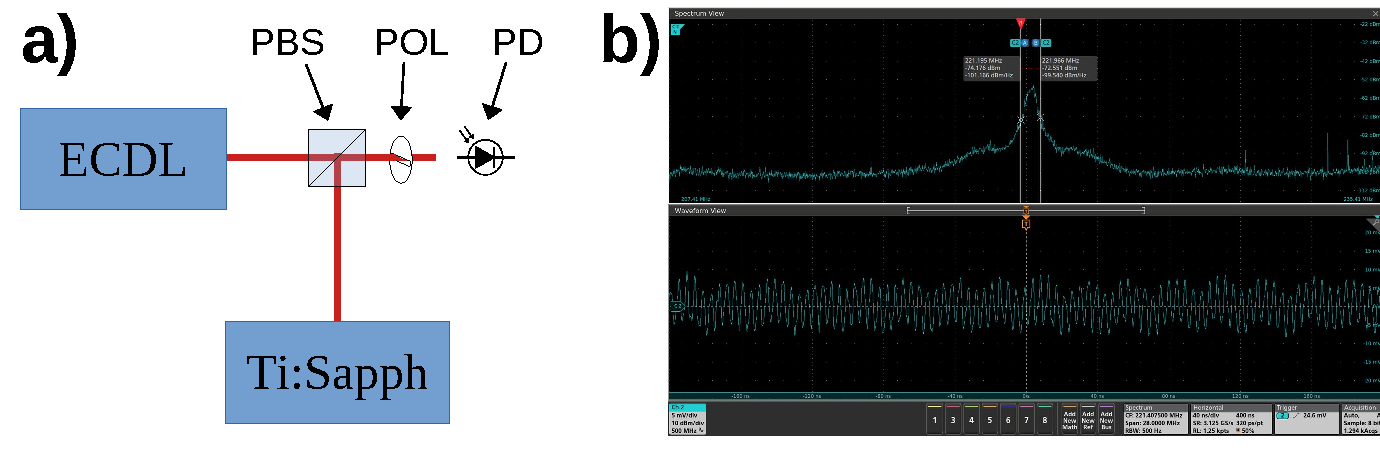
\includegraphics[width=1.0\linewidth]{diagrams/beatNote_cw-cw}
	\caption{Measurement of the optical beat note between two CW lasers. This is done by spatially overlapping the beams in the manner shown in \textbf{a)} using a polarizing beam splitter (PBS) and a polarizer (POL) to project the orthogonal polarizations onto the same axis. The overlapped beams have their intensity value measured by the fast photodiode (PD) which gives a strong oscillating signal when the two CW lasers have their optical frequency very close. The recording of this beat note is shown in \textbf{b)}, where both the time domain and frequency domain traces are shown simultaneously using a Tektronix MSO58 mixed-signal oscilloscope. In the upper portion is the output of the spectrum analyzer which shows an RF peak centered at 221.6 MHz. The lower portion is the time domain trace after the DC offset has been removed. It can be seen that the beat note oscillations are pronounced enough to be counted.}
	\label{fig:wl_beatnote_cw-cw}
\end{figure}

\section{Paraxial Wave Equation and Laser Beam Profiles} \label{sec:paraxial_approx}

The purpose of this section is to develop the Gaussian beam solution to Maxwell’s equations under the paraxial approximation and to introduce the complex $q$-parameter formalism that is essential for understanding optical cavities used in cavity-enhanced absorption spectroscopy techniques such as CRDS and Vernier spectroscopy.

By deriving solutions to the paraxial wave equation, we provide the necessary mathematical basis for the more advanced concepts discussed elsewhere in this dissertation, specifically regarding cavity path-length enhancement and the requirements for precise mode-matching. While the Fresnel integral provides a general method for calculating diffraction, the focus here is on the development of the complex $q$-parameter formalism, which provides a far more compact and physically transparent description of beam propagation that is essential for understanding optical cavities. This approach culminates in the introduction of the ray transfer matrix ($ABCD$) mathematics.

\subsection{Paraxial Wave Equation}
In a vacuum free of charges and currents, the electromagnetic field is governed by the Maxwell wave equation:
\begin{equation}
	\left(\nabla^2 - \frac{1}{c^2}\frac{\partial^2}{\partial t^2}\right)\mathbf{E}(\mathbf{r}, t) = 0
\end{equation}
For monochromatic waves of the form $\mathbf{E}(\mathbf{r},t) = \mathbf{E}(\mathbf{r})e^{-i\omega t}$, this reduces to the homogeneous Helmholtz equation:
\begin{equation} \label{helmholtz}
	\nabla^2 E + k^2 E = 0
\end{equation}
A general solution to the Helmholtz equation can be constructed via the Huygens-Fresnel principle, which treats any aperture as a collection of secondary spherical wavefronts originating from every point on the aperture surface. The field at a distance $d$ is given by the superposition:
\begin{equation}
	E(x,y,z=d) = -\frac{i}{\lambda}\int\int dx' dy' E(x',y',z=0) \frac{e^{i\mathbf{k}\cdot\mathbf{r}}}{R} \left[ \frac{1-\cos(\mathbf{\hat{r}},\mathbf{\hat{z}})}{2}\right]
\end{equation}
where the term in the brackets is the obliquity factor introduced by Kirchhoff to remove backward-travelling waves.

In most laser-based spectroscopic applications, we operate in the Fresnel regime, where the distance from the aperture is much greater than the aperture size itself ($d \gg \sqrt{(x-x')^2 + (y-y')^2}$). In this limit, we can approximate the wavefront as nearly planar ($R \approx d$) and the obliquity factor as unity. This simplifies the propagation to the Fresnel integral:
\begin{equation} \label{fresnel_integral}
	E(x,y,{z=d}) \,=\, \frac{-i}{\lambda d}e^{ikd} e^{\frac{ik}{2d}(x^2+y^2)}\int\int dx' dy' E(x',y',z=0) e^{\frac{-ik}{2d} (x'^2 + y'^2)} e^{\frac{ik}{d} (x x' + y y')}
\end{equation}
While the Fresnel integral provides a powerful method for calculating diffraction patterns, it is computationally intensive. To describe the smooth evolution of a laser beam more efficiently, we seek a streamlined approach by applying the \textit{paraxial approximation} directly to the Helmholtz equation. This yields the Paraxial Wave Equation (PWE), a differential equation that the Fresnel integral satisfies.

We consider a beam that maintains a well-defined direction along the $z$-axis. We use the ansatz
\begin{equation}
	E(\mathbf{r}) = E_0(\mathbf{r}) e^{ikz}
\end{equation}
to distinguish between the rapidly oscillating carrier wave and $E_0(\mathbf{r})$, a slowly varying spatial envelope. Substituting this into (\ref{helmholtz}) yields:
\begin{align}
	\left(\frac{\partial^2}{\partial x^2} + \frac{\partial^2}{\partial y^2} + \frac{\partial^2}{\partial z^2}\right)E_0 e^{ikz} + k^2 E_0 e^{ikz} &= 0 \nonumber\\
	\Bigg[\nabla_{\perp}^2 E_0 + \underbrace{\frac{\partial^2 E_0}{\partial z^2}}_{\mathclap{\begin{matrix}\approx 0\;\mathrm{parax.}\end{matrix}}}
	+ 2ik\frac{\partial E_0}{\partial z} - \cancel{k^2 E_0} + \cancel{k^2 E_0} \Bigg] e^{ikz} &= 0
\end{align}
where $\nabla_{\perp}^2 \equiv \partial^2/\partial x^2 + \partial^2/\partial y^2$. The paraxial approximation is valid when the envelope $E_0$ varies slowly along the direction of propagation, such that $\left|2k\frac{\partial E_0}{\partial z}\right| \gg \left|\frac{\partial^2 E_0}{\partial z^2}\right|$. Neglecting this second-order longitudinal derivative term leads to the Paraxial Wave Equation (PWE):
\begin{equation}\label{parax}
	\nabla_{\perp}^2 E_0 + 2ik\frac{\partial E_0}{\partial z} = 0
\end{equation}

\section{Connection to the Schrödinger Equation}

Through an appropriate change of variables, the paraxial wave equation (\ref{parax}) is mathematically isomorphic to the two-dimensional, time-dependent Schrodinger equation for a particle of mass $m$ (where $z$ plays the role of time) under the influence of an isotropic two-dimensional harmonic oscillator \cite{gaussBeam_schrodinger, diss_Strohaber2007}.

If we factor out a Gaussian dependence of the transverse profile in the form
\begin{equation}
	E_0(x,y,z) = \frac{w_0}{w(z)} f(\zeta,\eta,t)
	\exp\left(\frac{ik r^2}{2R(z)}\right)
\end{equation}
as well as introduce the scaled transverse coordinates $\zeta$, $\eta$, and the choice of the parameter $t'(z)$, analogous to time,
%	\begin{align}
	%		{t'} = \tan^{-1}\left(\frac{z}{z_R}\right) &&
	%		\frac{d{t'}}{dz} = \frac{w_0^2}{w^2 z_R}
	%	\end{align}
\begin{align}
	\zeta = \frac{\sqrt{2}x}{w(z)} &&
	\eta = \frac{\sqrt{2}y}{w(z)} && 
	{t'} = \tan^{-1}\left(\frac{z}{z_R}\right) &&
	\frac{d{t'}}{dz} = \frac{w_0^2}{w^2 z_R}
\end{align}
then the function $f(\zeta, \eta)$ gives the transverse profile of the beam as the Schrodinger equation
\begin{equation}
	\label{schrodinger_form}
	\left(
	\partial_{\zeta\zeta} + \partial_{\eta\eta}
	- \zeta^2 - \eta^2 + 2i\partial_{t'}
	\right) f = 0
\end{equation}

This is formally identical to the Schrödinger equation for a two-dimensional isotropic harmonic oscillator, with ${t'}(z)$ playing the role of time. This mapping allows us to treat the spatial evolution of a laser beam as a temporal evolution of a quantum state. Physically we can think of intercepting a laser beam with a piece of paper and viewing the transverse profile. As we move this paper along the beam propagation direction with a constant velocity, the profile exhibited by the beam on the paper evolves in space just as the 2D quantum harmonic oscillator evolves in time. For well-behaved laser, we excpect this oscillator to be in the ground state.

\subsection{Natural Basis of Beam Description}
The Schrodinger equation (\ref{schrodinger_form}) describing the transverse beam profile $f(\zeta, \eta)$ is separable in the three different coordinate systems \cite{schrodinger_2dho_separability}. These correspond to the fundamental modes of laser propagation.

In Cartesian coordinates, (\ref{schrodinger_form}) becomes separable using the ansatz
\begin{equation}
	f(\zeta,\eta,t) = A(\zeta,t)\,B(\eta,t)
\end{equation}
leads to two identical one-dimensional equations
\begin{equation}
	A_{\zeta\zeta} - \zeta^2 A + 2i A_t = 0
	\qquad
	B_{\eta\eta} - \eta^2 B + 2i B_t = 0
\end{equation}

Focusing on $A(\zeta,t)$ and separating variables in $\zeta$ and $t$, the spatial part satisfies
\begin{equation}
	\frac{d^2 A}{d\zeta^2} - \zeta^2 A + \lambda A = 0
\end{equation}
Which gives physically acceptable solutions as a Gaussian multiplied by a Hermite polynomial $H_n(\zeta)$
\begin{align}
	A(\zeta) = e^{-\zeta^2/2} H_n(\zeta) & & H_n(\zeta) = (-1)^n e^{\zeta^2}\frac{d^n}{d\zeta^n}e^{-\zeta^2}
\end{align}

\subsection{Transverse Mode Structure}

The transverse field distribution is therefore determined by solutions of the Schrodinger equation of the 2D isotropic oscillator. There are three natural basis sets to describe these solutions corresponding to the coordinate systems in which this problem is separable. 

Solutions to the paraxial equation in Cartesian coordinates $(\zeta, \eta)$ yield Hermite-Gaussian modes
\begin{equation}
	E_{nm}(x,y,z) \propto H_n(\text{scaled } x)H_m(\text{scaled } y)\exp(-\text{Gaussian envelope})
\end{equation}
while cylindrical $(r, \theta)$ coordinates yield Laguerre-Gaussian modes
\begin{equation}
	E_{pl}(r,\theta,z) \propto L_p^l(\text{scaled } r)\exp(il\theta)\exp(-\text{Gaussian envelope})
\end{equation}
Laguerre-Gaussian modes carry orbital angular momentum (OAM), while Hermite-Gaussian modes form a convenient basis for rectangular symmetry.

In this work, these higher-order modes are primarily relevant in the context of cavity alignment and mode-matching. Usually this misalignment occurs in the Cartesian directions, as opposed to some circularly varying phase delay. Therefore, the Hermite-Gauss modes form a natural basis for describing this misalignment. Efficient coupling into an optical cavity requires excitation of the fundamental $\mathrm{TEM}_{00}$ Gaussian mode; coupling into higher-order HG modes represent a rectangular misalignment of the cavity or input beam, leading to reduced coupling efficiency. For the purposes of cavity enhancement and mode-matching, we can therefore focus on the evolution of the Gaussian envelope itself. The Gaussian beam corresponds to the lowest-order HG solution ($n=m=0$), while higher-order modes arise as excited states of the same underlying Schrödinger-like system.

This formulation makes clear that the Gaussian beam is the fundamental, minimum-divergence solution of the paraxial wave equation (the isotropic oscillator only has one ground state solution, a Gaussian), and that higher-order transverse modes form a complete orthogonal basis determined by the symmetry of the coordinate system.

\section{Gaussian Beam Solution}

The fundamental TEM$_{00}$ solution to the paraxial equation is the Gaussian beam
\begin{equation} \label{gauss_TEM00}
	E_0(r,z) \propto \frac{w_0}{w(z)} \exp\left(-\frac{r^2}{w^2(z)}\right)
	\exp\left(i\frac{kr^2}{2R(z)} - i\psi(z)\right),
\end{equation}
It is convenient to make the identification of the following parameters, as they will be used frequently throughout this work
\begin{itemize}
	\item $w(z)$ is the \textbf{beam radius} at any location $z$ along the beam propagation direction
	\item $R(z)$ is the \textbf{wavefront radius of curvature}
	\item $\psi(z)$ is the \textbf{Gouy phase}
	\item $z_\mathrm{R}$ is the \textbf{Rayleigh range}, determined by the size of the beam waist
\end{itemize}
For a beam which comes to a focus at $z=0$, where $w(0) = w_0$ is the size of this waist, these quantities are respectively given by
\begin{align}
	w(z) &= w_0 \sqrt{1 + \left(\frac{z}{z_R}\right)^2} \\
	R(z) &= z\left[1 + \left(\frac{z_R}{z}\right)^2\right] \\
	\psi(z) &= \tan^{-1}\left(\frac{z}{z_R}\right) \\
	z_\mathrm{R} &= \pi n_r w_0^2/\lambda
\end{align}

Although the refractive index $n_r$ makes an appearance in the expression for $z_\mathrm{R}$, we will treat this as always being close to unity $n_r\simeq 1$, as the transition between media of differing refractive indices will be unimportant for this work.

\section{The Complex $q$-Parameter and Laser Beam Profile}

For a beam having a fundamental $\mathrm{TEM}_{00}$ solution with waist located at $z=0$, the field can be expressed compactly using the complex parameter $q(z)$:
\begin{equation}\label{gauss_TEM00-q}
	E_0(r,z) = E_0 \frac{w_0}{w(z)} \exp\left( -\frac{r^2}{w^2(z)} \right) \exp\left( i \left[ k z + \text{arg}(q(z)) \right] \right)
\end{equation}
where the phase evolution is intrinsically linked to the argument of $q$. Rather than treating $w(z)$ and $R(z)$ separately, it is convenient to define the complex beam parameter
\begin{equation}\label{complex_q}
	q(z) = z + i z_R.
\end{equation}
where its reciprocal encodes both geometric properties
\begin{equation} \label{compex_q_recip}
	\frac{1}{q(z)} = \frac{1}{R(z)} - \frac{i\lambda}{\pi n_r w^2(z)}.
\end{equation}

The utility of the complex $q$-parameter lies in its ability to encode the entire transverse state of a Gaussian beam into a single complex scalar via the  intensity profile $w(z)$ and the phase front curvature $R(z)$. Because the $1/q$ relation maps the physical properties of the beam onto the real and imaginary parts of a complex value, any linear optical transformation that affects the beam's geometry can be expressed as a transformation of $q$. For this work, we will use the vacuum refractive index $n_r = 1$.

\subsection{Ray Transfer Matrix Formalism}

The propagation of a Gaussian beam through an optical system can be represented by a single effective matrix $\mathbf{M}$ constructed from the product of individual element matrices:
\begin{equation}
	\begin{pmatrix} A & B \\ C & D \end{pmatrix} = \mathbf{M}_n \dots \mathbf{M}_2 \mathbf{M}_1
\end{equation}
The transformation of the $q$-parameter through such a system is given by the Möbius transformation:
\begin{equation} \label{gauss_complex_q_ABCD}
	q_{\text{out}} = \frac{Aq_{\text{in}} + B}{Cq_{\text{in}} + D}
\end{equation}
This formulism is convenient for the next chapter, where we will apply these matrices to determine the stability and eigenmode properties of the optical cavities used for ultra-sensitive absorption measurements.

\subsubsection{Ray Optical Analogy}
In classical ray optics, the propagation of a light ray through a system of lenses and mirrors is also described by the ray transfer matrices \cite{book_lasers_siegman} which take the same form as the $ABCD$ matrices. These track the evolution of a ray's position ($x$) and angle ($\theta$) from the optical axis through interactions in an optical system. Since a Gaussian beam can be similarly be viewed as a collection of rays concentrated around the optical axis (see Eq. \ref{fresnel_integral}), it is natural to ask how the $q$-parameter evolves when subjected to these same linear transformations.

The transition from the physical parameters $R(z)$ and $w(z)$ to the matrix formalism is made seamless by recognizing that the ray transfer $ABCD$ matrix acts on the complex $q$-parameter through a fractional linear transformation (or Möbius transformation). This allows us to bypass the cumbersome tracking of $R(z)$ and $w(z)$ through every lens and mirror in a complex setup, instead treating the entire optical train as a single operator acting on the initial beam state.

Consider how a single optical element transforms the transverse geometry of the beam. In ray optics, the state of a ray is defined by its distance $x$ and $\theta$ from the $z$-axis. For a paraxial ray ($\theta\sim0$), the transformation through an element $\mathbf{M}$ is:
\begin{align}
	\begin{pmatrix} x_{\text{out}} \\ \theta_{\text{out}} \end{pmatrix} = \begin{pmatrix} A & B \\ C & D \end{pmatrix} \begin{pmatrix} x_{\text{in}} \\ \theta_{\text{in}} \end{pmatrix}
\end{align}
The complex $q$-parameter is related to the ray's wavefront curvature. Specifically, for a beam propagating along $z$, the phase term $\exp(ikx^2/2R)$ in (\ref{gauss_TEM00}) implies that the angular divergence of the rays at the beam axis is intrinsically linked to the derivative of this phase.

The action of the $ABCD$ matrix on the complex $q$-parameter via Eq. (\ref{gauss_complex_q_ABCD}) represents a linear transformation of the underlying ray-optical phase-space coordinates $(x, \theta)$. In this representation, the real and imaginary parts correspond to the beam's wavefront curvature ($1/R$) and its transverse area ($\propto 1/w^2$). The $ABCD$ matrix acts on these components such that the "area" in this complex space--the product of the curvature and the beam area, $R \cdot w^2$--is conserved. This is a direct manifestation of Liouville’s theorem; the phase space volume preserves the fundamental structural relationship between the beam's divergence and its waist. Consequently, the unimodular constraint
\begin{equation}
	\det \mathbf{M} = 1
\end{equation}
ensures that while the beam may expand or contract, the quadratic phase structure required to maintain a Gaussian profile remains intact throughout propagation.

\section{Stable Optical Cavity Geometry}
A fundamental application of this formalism is the description of optical cavities. In a cavity, the field must be self-consistent; that is, the Gaussian beam describing the intracavity field must remain invariant after a single round trip. Using the $ABCD$ law (\ref{gauss_complex_q_ABCD}), this condition is expressed as a fixed-point equation for the complex beam parameter
\begin{equation} \label{cav_eigenvalue}
	q = \frac{Aq + B}{Cq + D}
\end{equation}
Solutions to this equation define the cavity eigenmodes. To investigate the stability of such a system, it is computationally convenient to solve for the reciprocal of the complex $q$-parameter. By forming $1/q$ in the fixed-point relation (\ref{cav_eigenvalue}), we can reformulate the stability condition as a quadratic equation
\begin{equation}
	B\left(\frac{1}{q_\mathrm{eig}}\right)^2 + (A-D)\left(\frac{1}{q_\mathrm{eig}}\right) - C = 0
\end{equation}
This gives two solutions for the reciprocal of the complex q-parameter of the cavity eigenmode
\begin{equation}
	\frac{1}{q_\mathrm{eig}} = \frac{D-A}{2B} \pm \frac{1}{B}\sqrt{\frac{(D-A)^2}{4} + BC}
\end{equation}
The solution is chosen such that the imaginary part is negative to agree with (\ref{compex_q_recip}). Using the unimodularity condition $AD - BC = 1$, we then have for the complex $q$-parameter of the cavity eigenmode
\begin{equation} \label{cavity_eigenmode_recip}
	\frac{1}{q_\mathrm{eig}} = \frac{A-D}{2B} - \frac{i}{|B|}\sqrt{1 - \frac{1}{4}\left(D + A\right)^2}
\end{equation}
The waist size and location can be determined by equating the real and imaginary parts of (\ref{complex_q}) to those of $q_\mathrm{eig}$. While these can be found by taking the reciprocal of above for $1/q_\mathrm{eig}$, it is much easier to re-arrange the quadratic equation (\ref{cav_eigenvalue}) to give $cq_\mathrm{eig}^2 + (D-A)q_\mathrm{eig} -B = 0$, and the solution
\begin{equation}\label{cavity_eigenmode}
	q_\mathrm{eig} = \frac{A-D}{2C} + \frac{i}{|C|}\sqrt{1-\frac{1}{4}(D+A)^2}
\end{equation}
The stability of the cavity--the condition that a physical, finite beam waist exists--requires that the term under the radical remains positive. This yields the fundamental stability criterion for an optical cavity
\begin{equation} \label{cavity_stab_condition}
	\left|D+A\right| \leq 2
\end{equation}
where the values of $A$ and $D$ come from the round-trip $ABCD$ ray transfer matrix.

\section{ABCD Matrices of Cavity Elements and Configurations}
The configuration of mirrors and non-refractive focusing optics common in the construction of cavities are represented by the ray-transfer $ABCD$ matrices	
\begin{itemize}
	\item Free Space Propagation
	\begin{equation} \label{mat_prop}
		\mathbf{P}_d = 
		\begin{pmatrix}
			1 & d \\
			0 & 1
		\end{pmatrix}
	\end{equation}
	\item Flat Mirror Reflection
	\begin{equation*}
		\mathbf{M} = 
		\begin{pmatrix}
			1 & 0 \\
			0 & 1
		\end{pmatrix}
	\end{equation*}
	\item Curved Mirror Reflection
	\begin{equation*}
		\mathbf{M}_R = 
		\begin{pmatrix}
			1 & 0 \\
			-\frac{2}{R} & 1
		\end{pmatrix}
	\end{equation*}
\end{itemize}

For the optical cavities considered in this work, the beam does not cross any refractive index boundaries in the cavity round-trip. Due to Fresnel reflections, this is usually to be avoided. For this reason, we have considered the refractive index throughout this work to be unity $n_r = 1$. While refractive index boundaries can be effectively modeled using the ray-transfer matrix formulism, it should be pointed out that there are effectively two different approaches for the propagation of a Gaussian beam:
\begin{itemize}
	\item Using a ray transfer matrix to explicitly show the change in direction across the boundary having ratio of refractive indices $n$. This is the diagonal ABCD matrix having $A=1$ and $D=1/n$, which is equivalent to the transformation $q' = nq$. The beam radius calculation must then undo this transformation by $w' = w/ \sqrt{n}$.
	
	\item Transform all propagation distances inside the medium by an amount $d' = d/n$.
\end{itemize}

\noindent
Such considerations may be used, for instance, in the atigmatic compensation of ring cavities, where the inclusion of a Brewster-angled refractive element can compensate for the astigmatism introduced by the angled focusing mirrors \cite{book_ultrashort_lp_phenom_CH5}. For the remainder of this work, however, we will take the refractive index to be that of the vacuum without any refractive index boundaries. 

\subsection{Linear Optical Cavity} \label{sec:cav_ABCD}
The simplest linear optical cavity consists of two mirrors separated by a distance $L$, as in Fig. \ref{fig:cavitylinear}. We will later show how a small absorption can be greatly amplified using an optical cavity. This absorption signal manifests itself as a change in the round-trip loss. A cavity which has low intrinsic losses is then naturally able to measure small changes in intra-cavity absorption. When the mirror reflectivity is the limiting factor in this round-trip loss, the number of reflections should be minimized. The simple linear cavity has the fewest number of reflections.

\begin{figure}[H]
	\centering
	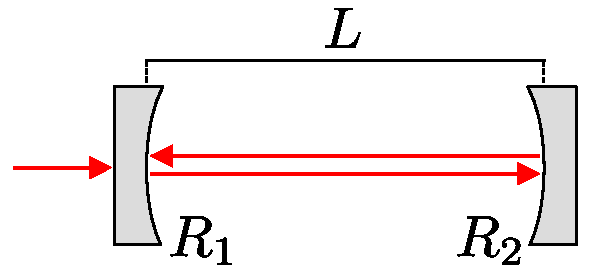
\includegraphics[width=0.3\linewidth]{diagrams/cavity_linear}
	\caption{Simple linear optical cavity constructed from two mirrors having radii of curvature $R_{1,2}$ and separation distance $L$.}
	\label{fig:cavitylinear}
\end{figure}

We consider a cavity consisting of two mirrors having radii of curvature $R_1$ and $R_2$ separated by a distance $L$. Using the ray transfer matrices (\ref{mat_prop}), we represent the propagation from one mirror to the other as the matrix $\mathbf{P}_L = \begin{pmatrix} 1 & L \\ 0 & 1 \end{pmatrix}$ and the mirror reflections as $\mathbf{M}_{1,2} = \begin{pmatrix} 1 & 0 \\ -2/R_{1,2} & 1 \end{pmatrix}$. Starting from the mirror having curvature $R_1$, the $ABCD$ matrix representing the round trip of the cavity is
\begin{equation}
	\begin{pmatrix}
		A & B \\
		C & D
	\end{pmatrix}
	=
	\mathbf{M}_1 \, \mathbf{P}_L \, \mathbf{M}_2 \, \mathbf{P}_L
\end{equation}
The coefficients of the resulting transfer matrix are
\begin{align}
	A &= 1 - \frac{2L}{R_2} & 
	B &= L\left(2 - \frac{2L}{R_2}\right) \\
	C &= -\frac{2}{R_2} + \frac{2}{R_1}\left(\frac{2L}{R_2} - 1\right) & 
	D &= 1- \frac{2L}{R_2} - \frac{2L}{R_1}\left(2 - \frac{2L}{R_2}\right)
\end{align}
If we introduce the dimensionless parameter $g_{1,2} = 1 - L/R_{1,2}$, then the matrix elements become
\begin{align}
	A &= 2g_2-1 & B &= 2Lg_2 \\
	C &= \frac{2}{L}\left(2g_1g_2 - g_1 - g_2\right) & D &= 4g_1g_2 - 2g_2 -1
\end{align}
The stability condition $\left|A + D\right| \leq 2$ then reads
\begin{align}
	-2 \leq 4g_1g_2 - 2  \leq 2 \nonumber \\
	0 \leq g_1 g_2 \leq 1 \nonumber
\end{align}
The stability condition for the linear cavity can then be written as
\begin{equation}
	0 \leq \left(1 - \frac{L}{R_1}\right)\left(1 - \frac{L}{R_2}\right) \leq 1
\end{equation}

We can retrieve the beam radius at one of the mirrors by equating the imaginary part of (\ref{compex_q_recip}) to that of (\ref{cavity_eigenmode_recip}). The beam radius at mirror $R_1$ is then
\begin{align} \label{cavity_beamsize_m1}
	w_1^2 = \frac{\lambda}{\pi n} \Big/ \left(\frac{1}{|B|}\sqrt{1 - \frac{1}{4}(D+A)^2}\right)
	&= \frac{\lambda L}{\pi n}\sqrt{\frac{g_2}{g_1(1-g_1g_2)}}
	%\sqrt{\frac{\frac{\lambda}{\pi n}L(L-R)}{R_2\sqrt{L\left(1 - \frac{L}{R_1}\right)\left(1-\frac{L}{R_2}\right)\left(\frac{1}{R_1} + \frac{1}{R_2} - \frac{L}{R_1R_2}\right)}}}
\end{align}
We can repeat the computation for the round-trip ABCD matrix, but instead starting at mirror $R_2$. The new ABCD matrix would be the same, expect for the swapped $g_1 \leftrightarrow g_2$. With this in mind, we can immediately write the beam radius at mirror $R_2$ as
\begin{equation} \label{cavity_beamsize_m2}
	w_2^2 = \frac{\lambda L}{\pi n}\sqrt{\frac{g_1}{g_2(1-g_1g_2)}}
\end{equation}

When trying to mode-match an input beam to the cavity, it is useful to know the location of the beam waist and its size $w_0$. These are conveniently related through (\ref{complex_q}) to the cavity eigenmode. It can be easily seen that the waist size is given by
\begin{align} \label{cavity_w0}
	w_0^2 = \frac{\lambda}{\pi n}\mathrm{Im} \left[q_\mathrm{eig}\right] = \frac{\lambda}{\pi n} \frac{1}{|C|}\sqrt{1-\frac{1}{4}(D+A)^2} = \frac{\lambda L}{\pi n}\frac{\sqrt{g_1 g_2 (1-g_1g_2)}}{\left|2g_1g_2 - g_1 - g_2\right|}
\end{align}
The location of this waist relative to the position of mirror $R_1$ is simply the negative real part of the q-parameter for the cavity eigenmode
\begin{equation} \label{cavity_z0}
	z_0 = -\mathrm{Re}\left[q_\mathrm{eig}\right] = \frac{D-A}{2C} = L\frac{g_2(g_1 - 1)}{2g_1g_2 - g_1 - g_2}
\end{equation}

\subsubsection{Half-Symmetric Cavity}
A useful configuration for an optical cavity is the half-symmetric cavity, which has a flat mirror and a curved mirror having radius of curvature $R$. If we consider that the cavity round-trip is starting at the flat mirror, then according to our convention above we have
\begin{eqnarray}
	g_1 = 1 &\qquad& g_2 = 1 - \frac{L}{R} \equiv g
\end{eqnarray}
The location of the beam waist relative to the flat mirror is given by (\ref{cavity_z0}) and can be seen to be $z_0=0$. This means that the beam waist is located exactly at the flat mirror. The size of this waist is given by (\ref{cavity_w0}) and is given by
\begin{equation} \label{cavity_waste_size_half-sym}
	w_{0,\mathrm{HS}} = \frac{\lambda L}{\pi n}\sqrt{\frac{g}{1-g}}
	%= \frac{\lambda L}{\pi n}\frac{\sqrt{(1-L/R) (L/R)}}{\left|-L/R\right|}
	= \frac{\lambda L}{\pi n}\sqrt{\frac{R}{L}-1}
\end{equation}
The stability condition is easily seen to be $R > L$ for the half-symmetric cavity.

\subsection{Mode-Matching} \label{sec:mode-matching}
The most efficient coupling of a laser beam into an optical cavity is achieved by ensuring that the transverse profile of the beam matches the profile of the cavity eigenmode predicted by (\ref{cavity_eigenmode}). The fundamental $\mathrm{TEM}_{00}$ mode of the cavity has a Gaussian profile, and therefore the input beam should be free of higher order spatial modes. For lasers which have a poor beam profile, a spatial mode filter can be employed to clean up the beam at the expense of power. Once a clean Gaussian beam is achieved, it can be profiled using the knife-edge technique \cite{book_gaussBeams_AtomsMolsOpticalPhys2} or other beam profiling method. The ray transfer matrices (\ref{mat_prop}) can then be used to find a set of focusing elements which bring the laser beam profile into overlap with the cavity eigenmode.

We gave as an example the half-symmetric cavity, having a flat mirror as an input coupler and a curved mirror of radius $R$. We found that the cavity eigenmode has a waist which is located at the flat mirror with radius $w_0$ given by (\ref{cavity_waste_size_half-sym}). From equation (\ref{gauss_complex_q_ABCD}), we have the complex $q$-parameter $q(z)$ at every location $z$ in the cavity. From (\ref{compex_q_recip}), we find that the transverse profile of the beam follows the hyperbola
\begin{equation} \label{beam_hyperbola}
	w(z) = \sqrt{\frac{-\lambda}{\pi n \,\mathrm{Im} \left[\frac{1}{q(z)}\right]}} = w_0\sqrt{\left(\frac{z}{\pi n w_0^2 /\lambda}\right)^2 + 1}
\end{equation}
If the flat mirror is located at $z=0$ and the curved mirror is located at $z=L$, then the profile of the input beam must match what is predicted by the above equation for negative $z$ values. The profile of the input beam which is matched to a half-symmetric cavity is shown in Fig. \ref{fig:cavitymodematch}(a), where the cavity eigenmode is calculated using the parameters $L=1200$mm and $R=2000$mm.

In general, the input beam must match the cavity eigenmode extrapolated past the input coupler. A more complicated ring cavity configuration is shown in Fig. \ref{fig:cavitymodematch}(b), where the cavity eigenmode is seen to form two waists. The input beam profile can be calculated from equation (\ref{beam_hyperbola}) using the correct beam waist location and size.

\begin{figure}[H]
	\centering
	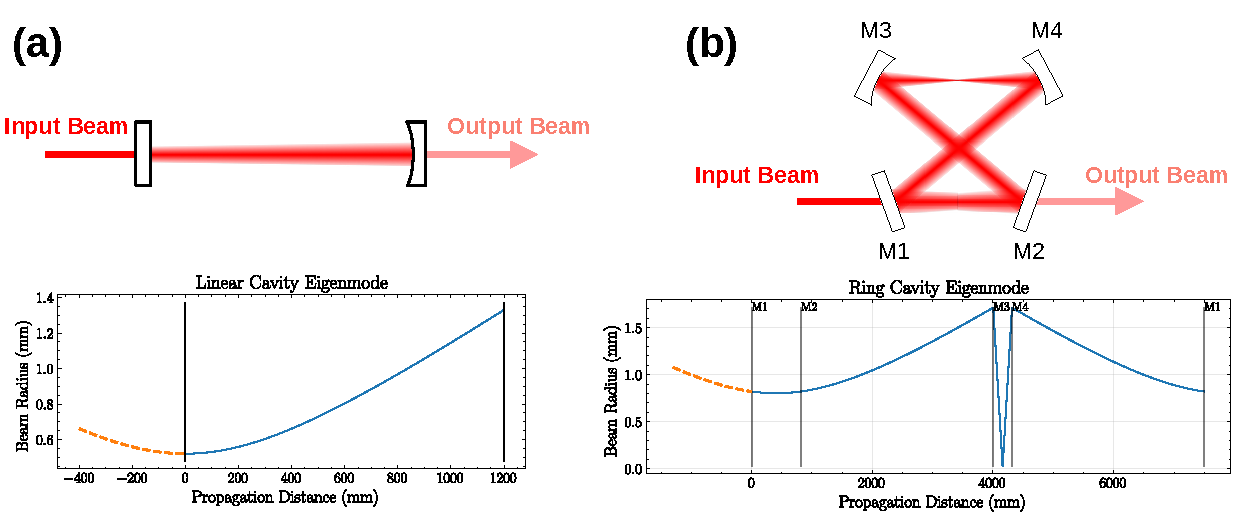
\includegraphics[width=1.0\linewidth]{diagrams/cavity_modeMatch}
	\caption{Shown are the calculated eigenmodes for two optical cavity configurations used in this work. The blue traces in the lower panes corresponds to the cavity eigenmode, and the dashed orange trace corresponds to the modematched input beam. For the half-symmetric linear cavity shown in \textbf{(a)}, the input coupler is a flat mirror and the waist of the eigenmode sits at the reflective surface. The output coupler is a curved mirror of radius $R=2$m located a distance $L=1.2$m away from the input coupler, and the wavefront radius of curvature of the eigenmode matches this value at the reflective interface. Shown in \textbf{(b)} is a ring cavity having the shown simplified configuration. Mirrors M1 and M2 are the flat input and output couplers. Mirrors M3 and M4 are concave mirrors having radius of curvature $R=300$mm. The eigenmode for this cavity forms two waists, one of tight focus halfway between the concave mirrors and another which is located away at one half the round trip distance of the cavity. The total length of the cavity gives $\mathrm{FSR} \sim 40\mathrm{MHz}$.}
	\label{fig:cavitymodematch}
\end{figure}

It should be noted that the linear cavity shown in Fig. \ref{fig:cavitymodematch}(a) has the property that the condition for mode-matching corresponds exactly to maximum back-reflectance of the input beam from the furthest mirror back into the laser source. For this reason, it is advised to use a form of optical isolator between the laser and a linear cavity to prevent this maximally back-reflected beam from entering back into the laser source. The ring cavity does not have this issue, since the beam returning from the cavity round-trip is pointing in a different direction than the input beam.	


\chapter{OPTICAL CAVITY DYNAMICS} \label{chap:cav_dynamics}

The practical application of cavity-enhanced spectroscopy relies on understanding how optical cavity systems respond to time-dependent perturbations. In applications such as Cavity Ring-Down Spectroscopy (CRDS) and Vernier spectroscopy, the experimental signal is not merely a steady-state transmission, but a complex transient response resulting from the dynamic interaction of cavity length and laser wavelength.

This chapter develops the mathematical framework required to model these dynamic interactions. We begin by deriving the steady-state Airy transmission function for a monochromatic input, establishing the fundamental relationships between cavity finesse, free spectral range (FSR), and resonance linewidth. Subsequently, we transition to the time domain, treating the cavity as a linear system characterized by a specific impulse response. Finally, we establish the theoretical basis for the transient decay models employed in this work by analyzing the convolution of this impulse response with various input waveforms, including rectangular pulses, frequency-swept signals, and length-modulated transients.

Ultimately, these derivations provide the analytical tools necessary to interpret the high-speed photodetector signals discussed in the other chapters, where these dynamic cavity responses are leveraged for the ultra-sensitive detection of trace molecular species in breath analysis applications.

\section{Steady State Intensity Transmitted by an Optical Cavity} \label{sec:cav_transmission}
We consider here monochromatic light incident on a stable optical cavity having length $L$ with input coupler located at $z=0$. The incoming light has Gaussian transverse profile $E_0(x,y,z)$, and we write the incident electric field as
\begin{equation}
	E_\mathrm{in}(x,y,z,t) = E_0(x,y,z) e^{i\omega t - kz}
\end{equation}
From the discussion in Sec. \ref{sec:paraxial_approx}, the transverse profile $E_0(x,y,z)$ obeys the paraxial wave equation (\ref{parax}) and therefore evolves as a Gaussian beam between the cavity mirrors.

For now we will assume perfect mode-matching where the transverse profile of the input beam has complex-$q$ parameter that matches the cavity eigenmode (\ref{cavity_eigenmode}) at the input coupler. It is then understood that the transverse profile at the output of the cavity $E_0(x,y,z=L)$ is that of a Gaussian beam having beam size (\ref{cavity_beamsize_m2}) with a waist of size (\ref{cavity_w0}) located a distance (\ref{cavity_z0}) from the input coupler. For a symmetric cavity the transverse profile of the output field exactly matches that of the input field.

For a more general cavity, the transverse field at a single point $E_0(x,y,0)$ on the input coupler is mapped to a corresponding point on the output coupler by a complex constant $E_0(x,y,L) = a(x,y)E_0(x,y,0)$. For the remainder of this section, we will only be concerning ourselves with the time dependence of a photodetector which is reading the intensity of the light integrated across the transverse profile of the beam. Since the integrated intensity is unaffected by the beam size, equivalent to the condition $\int\int\left(\left|a(x,y)\right|^2 -1\right)\left|E_0(x,y,0)\right|^2 dx dy = 0$, we will simply take $a=1$ with the understanding that the detailed transverse profile at the output coupler has additional complex factor in front which does not affect the integrated intensity for non-symmetric cavities.

As shown in Fig \ref{fig:cavitytransmission}b, the incident light makes a single pass through the cavity encountering two mirror transmissions and a phase factor from the distance $L$ of propagation. The mirrors are characterized by their reflection coefficient $r$ and transmission coefficient $t$, which give the transmitted and reflected electric field as $tE$ and $rE$, respectively, as shown in Fig. \ref{fig:cavitytransmission}a. In general these coefficients are complex, allowing for a phase shift of the field in transmission and reflection. This contributes part of the output as $E_\mathrm{in} t^2 e^{-i\omega L/c}$. At the second cavity mirror, the single pass beam is reflected twice and encounters a phase factor from the $2L$ propagation distance giving an additional output of $E_\mathrm{in} t^2 e^{-i\omega L/c} r^2 e^{-2i\omega L/c}$. The total output of the cavity is the sum of the infinitely many contributions from successive number of round trips.
\begin{figure}[H]
	\centering
	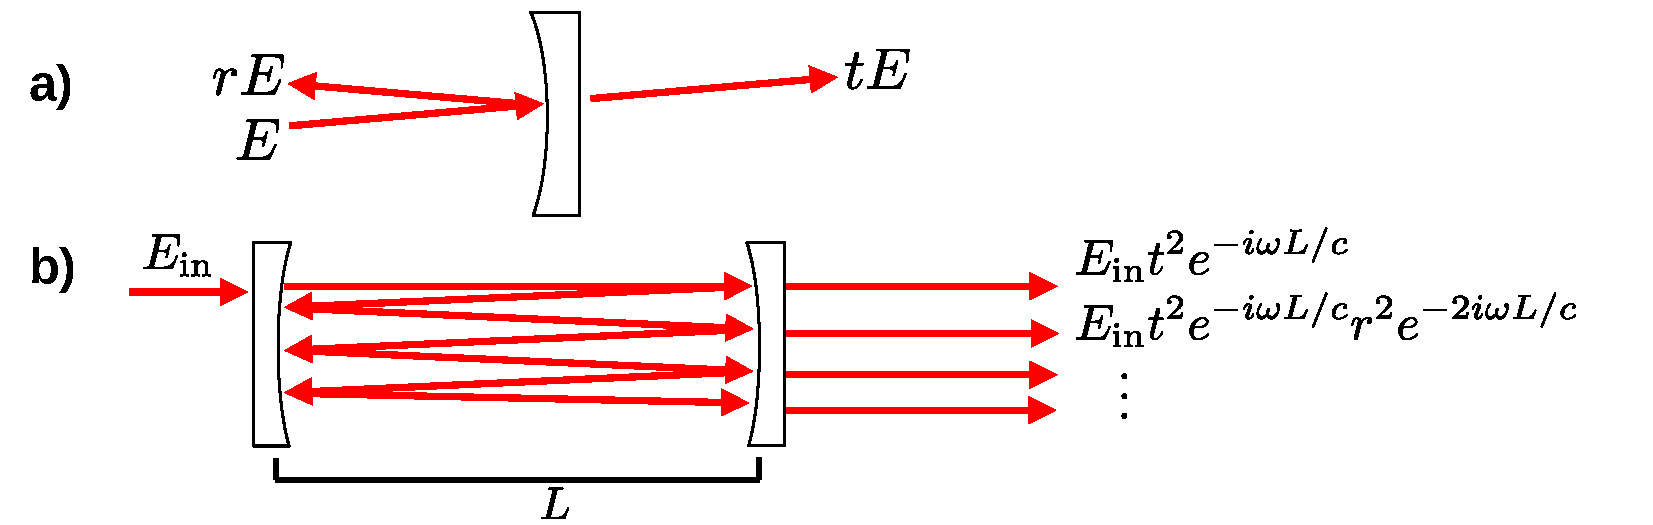
\includegraphics[width=0.7\linewidth]{diagrams/cavityTransmission}
	\caption{In \textbf{a)} is shown the complex coefficients of reflection $r$ and transmission $t$ which act to attenuate and phase shift the incident wave having field $E$. In \textbf{b)} the process of summing the many cavity round trips is illustrated. The output of the cavity is a sum of the single pass and the infinitely many round trips.}
	\label{fig:cavitytransmission}
\end{figure}

The output of the cavity is given by the sum
\begin{align} \label{cav_E-sum}
	E_\mathrm{out}(\omega) &= E_\mathrm{in}(\omega) t^2 e^{-i\omega L/c} \sum_{m=0}^\infty r^{2m} e^{-2im\omega L/c} \nonumber \\
	&=E_\mathrm{in}(\omega)\frac{t^2 e^{-i\omega L/c}}{1-r^2 e^{-i\omega t_r}}
\end{align}
In writing the above expression we have used the geometric series $\sum_{m=0}^\infty x^m = 1/(1-x)$, which is valid since $\left|r\right| < 1$ by definition. We have also defined the round-trip traversal time of the cavity $t_r = 2L/c$. The time-averaged intensity seen by a photodetector is given by $E_\mathrm{out}^* E_\mathrm{out}$.
\begin{equation} \label{_cav_I_comp}
	I_\mathrm{out} = I_\mathrm{in} \frac{T^2}{\left|1 - r^2 e^{-i\omega t_r}\right|^2}
\end{equation}
Above we have defined the coefficient $T$ for transmitted light intensity as $\left|t\right|^2 = T$. The complex number $r^2$ is written in terms of a real-valued intensity reflectivity value $R$ and a round-trip phase shift $2\phi$ of the twice reflected electric field
\begin{equation} \label{cav_R_defin}
	r^2 = Re^{-2i\phi}
\end{equation}
The denominator term of (\ref{_cav_I_comp}) is real and this can be reflected switching from complex exponentials to the trigonometric functions
\begin{equation}
	\left|1 - R e^{-i\omega t_r - 2\phi}\right|^2 = 1 + R^2 - 2R\cos(\omega t_r + 2\phi) = (1-R)^2 + 4R\sin^2(\frac{\omega t_r}{2} + \phi)
\end{equation}
We then arrive at the well known Airy formula for the transmitted light Intensity
\begin{equation}\label{cav_airy}
	I_\mathrm{out}(\omega) = \frac{T^2}{(1-R)^2}\frac{1}{1 + \frac{4R}{(1-R)^2}\sin^2\left(\frac{\omega t_r}{2} + \phi\right)} I_\mathrm{in}(\omega)
\end{equation}
The transmission function is a set of evenly spaced resonances when there is no frequency dependence of the reflection phase shift $\phi$. The maximum transmission occurs when the argument to the sine function is an integer multiple of $\pi$, so we have for integer $m$
\begin{align} \label{cav_resonance_condition}
	\frac{\omega L}{c} + \phi(\omega) = m \pi
\end{align}
If we solve for the cavity length $L$ in terms of the wavelength, the mirror separations which give resonance with a laser of wavelength $\lambda$ are evenly spaced in half-integer multiples of this wavelength
\begin{align} \label{cav_resonance_length}
	L = \frac{1}{2}\left(m - \frac{\phi(\lambda)}{\pi}\right)\lambda
\end{align}
The free spectral range (FSR) is given by the spacing of these resonances. For $\phi(\omega)$ being constant between the two resonances, the FSR is given in the optical frequency $\nu$ by
\begin{equation}
	\mathrm{FSR} = \frac{1}{t_r}
\end{equation}
The FWHM width of each resonance in the cavity transmission function (\ref{cav_airy}) is easily found to be
\begin{equation}
	\Delta \nu = \frac{2}{\pi t_r} \sin^{-1}\left(\frac{1-R}{2\sqrt{R}}\right)
	\sim \frac{1}{\pi t_r}\frac{1-R}{\sqrt{R}}
\end{equation}
Note that the above expression is the FWHM in the optical frequency $\nu$, as opposed to the earlier expressions using the angular frequency $\omega = 2\pi \nu$. The approximation made on the right of the expression above is valid for cavity mirrors having high reflectivity $R\sim 1$. In this limit, the cavity resonances look approximately like a Lorentzian near the transmission peak with the resonances becoming narrower for larger reflectivity. We can also define the cavity finesse as the ratio of the free spectral range (FSR) to the width of the resonance
\begin{equation}
	\mathcal{F} = \frac{\mathrm{FSR}}{\Delta\nu} = \pi \frac{\sqrt{R}}{1-R}
\end{equation}
This dimensionless parameter is a sort of quality factor which is only determined by round-trip loss of the field inside the cavity. This sensitivity to the loss can be exploited in cavity mode-width spectroscopy \cite{crds_cavityModeWidth_Cygan} to detect intracavity absorption.

\section{Ring-down Time}
For an optical cavity of sufficiently low loss, it is possible to observe the "ring-down" of light trapped between the mirrors after the laser coupling energy into the cavity has been shut off. This occurs because the light circulating between the mirrors propagates at a finite speed and takes a measurable amount of time for the light to leak out of the cavity mirrors. The response of the cavity to an arbitrary time dependent field is given, and then approximations are made for the case where the input field takes the form of a short pulse. This allows us to derive an analytic expression for the characteristic time of cavity ring-down.

The cavity response in equation (\ref{cav_E-sum}) is linear in the input field and takes the form of a transfer function $E_\mathrm{out}(\omega) = E_\mathrm{in}(\omega) H(\omega)$ in frequency space. The response of the cavity to an arbitrary input electric field $E_\mathrm{in}(t)$ is then the convolution with the inverse Fourier transform of the transfer function $\tilde{H}(t) = \mathcal{F}^{-1}(H(\omega))(t)$, giving
\begin{align} \label{cav_convolution}
	E_\mathrm{out}(t) = \int_{-\infty}^{\infty} E_\mathrm{in}(t-\tau) \tilde{H}(\tau) d\tau &&;&&
	\tilde{H}(t) = \frac{1}{2\pi}\int_{-\infty}^{\infty} e^{i\omega t}H(\omega) d\omega
\end{align}

We wish to find the response of the cavity to an impulsive input. From (\ref{cav_E-sum}) the transfer function is
\begin{equation}
	H(\omega) = T e^{-i\omega t_r/2} \sum_{m=0}^\infty r^{2m} e^{-im\omega t_r}
\end{equation}
Taking the transform of this expression is most easily done in this summation form. For a Dirac delta function input pulse, the output field is simply the impulse response $E_\mathrm{out}(t) = \tilde{H}(t)$. Taking the transform of the above expression and interchanging the sum and integrals
\begin{align} \label{cav_impulse_response}
	\tilde{H}(t)
	&= \frac{T}{2\pi} \sum_{m=0}^\infty r^{2m} \int_{-\infty}^{\infty} e^{i\omega t} e^{-i\omega t_r/2 -im\omega t_r} d\omega \\
	&= \frac{T}{2\pi} \sum_{m=0}^\infty \left(Re^{-2i\phi}\right)^{m}\int_{-\infty}^{\infty} e^{i\omega (t - t_r/2 - m t_r)} d\omega \\
	%&= T \sum_{m=0}^\infty R^{m} \delta(t - t_r/2 - m t_r) \\
	E_\mathrm{out}(t) &= T \sum_{m=0}^\infty \left(Re^{-2i\phi}\right)^{m} \delta(t - t_r/2 - m t_r)
\end{align}

The intensity of the cavity output light is proportional to $E^*_\mathrm{out} E_\mathrm{out}$, which gives
\begin{align}
	I_\mathrm{out}(t) &= T^2 \sum_{m=0}^\infty\sum_{n=0}^\infty R^{m+n} \delta(t - t_r/2 - m t_r)\delta(t - t_r/2 - n t_r) \nonumber \\
	&= T^2 \sum_{m=0}^\infty R^{2m} \delta^2(t - t_r/2 - m t_r)
\end{align}
We note that the second line is obtained by observing that the only non-zero terms of the nested sum are those for which $m=n$ due to the product of delta functions. This takes the form of a series of pulses separated in time by $t_r$ and are decaying in amplitude as the power of $R$ increases by two for each pulse. Physically this corresponds to a pulse circulating in the cavity, where a fraction of the pulse energy is transmitted out of the cavity on each round trip. The amplitude of these pulses follow the envelope
%	\begin{equation}
	%		E_\mathrm{out}(t) \approx T R^{t/t_r} = T e^{\ln(R) t/t_r}
	%	\end{equation}
%	The light intensity goes as the square of the field, so we have
\begin{equation}
	I_\mathrm{out}(t) \approx T^2R^{2t/t_r} = T^2 e^{\ln(R) 2t/t_r} \equiv I_0e^{-t/\tau_0}
\end{equation}
Above we have defined the ring-down time $\tau_0$ which is the $1/e$ characteristic decay time of the cavity output intensity. We can express this ringdown time as
\begin{equation} \label{tau_vac_exact}
	\tau_0 = \frac{-t_r}{2\ln R} = \frac{-L/c}{\ln R}
\end{equation}
If we use the approximation $\ln \left(R\right) = \ln(1 + (R - 1)) \approx R-1$ this becomes the well-known expression for the ring-down time of an empty symmetric cavity valid for high reflectivity mirrors.
\begin{equation} \label{tau_vac}
	\tau_0 = \frac{L/c}{1-R}
\end{equation}

If there is an absorbing gas species present in the space between the cavity mirrors having absorption coefficient $\alpha$ from (\ref{beer-lambert-law}), then each traversal across the distance $L$ between the mirrors gives an attenuation factor of $e^{-\alpha L/2}$ to the electric field. The factor of $1/2$ comes from considering the electric field instead of intensity. Combined with the losses already present from the mirror reflectivity, the round-trip attenuation factor becomes $r^2 e^{-\alpha L}$. To consider absorption in the cavity, we can simply replace the mirror reflectivity with $r^2 \rightarrow r^2 e^{-\alpha L}$. The phase shift of the reflectivity $\phi$ does not affect the output intensity for an impulsive input field, so we neglect this contribution. This leads us to replace the intensity reflectivity coefficient $R$ with
\begin{equation}
	R\rightarrow Re^{-\alpha L}
\end{equation}
Putting this substitution into (\ref{tau_vac_exact}), we obtain
\begin{equation}\label{tau_exact}
	\tau = \frac{-L/c}{\ln R - \alpha L}
\end{equation}
Again using the approximation of high reflectivity $R\sim 1$, we get the well-known expression for the ring-down time of a cavity with an absorbing gas
\begin{equation}\label{tau}
	\tau = \frac{L/c}{1-R + \alpha L}
\end{equation}
It is clear that the presence of an absorbing species lowers the ring-down time of the cavity.

\section{Transient Response of the Cavity} \label{sec:cav_td_response}
In this section, we consider the time dependence of the cavity output field to various input fields, which are chosen to more closely represent an achievable experiment using a CW laser mode-matched to the cavity than the results derived in the previous section using Dirac delta function field inputs.

Using our result for the impulse response of the cavity (\ref{cav_impulse_response}), we can compute the output for an arbitrary input electric field from the convolution in (\ref{cav_convolution}). Since the impulse response was found to be a sum of Dirac delta functions, the convolution integral reduces to a sum over the field value at previous times
\begin{equation} \label{cav_output_field}
	E_\mathrm{out}(t) = T \sum_{m=0}^{\infty} r^{2m} E_\mathrm{in} \left(t - \frac{t_r}{2} - m t_r\right)
\end{equation}
This result is exactly what would be expected if we had started writing the electric field in the time domain instead of the frequency domain and used the construction of Fig. \ref{fig:cavitytransmission} to write down the above sum instead of equation (\ref{cav_E-sum}). This time-domain response function is convenient for analyzing the transient response of the cavity, an understanding of which is critical for accurate determination of the ringdown time.

We begin by analyzing the case of a finite laser pulse having minimal spectral width coupled into the cavity. This will allow us to see the detailed buildup to the steady state response $I_\mathrm{out}(\omega)$ given by (\ref{cav_airy}), as well as the conditions under which the ringdown time (\ref{tau}) can be accurately measured.

\subsection{Response to a Finite Monochromatic Pulse}
For a finite monochromatic pulse of duration $D$, we can represent the input electric field using the step function $\theta(t) = \begin{cases}0 & t<0 \\1 &t>0 \end{cases}$ which gives for the pulsed field at the input of the cavity
\begin{equation}
	E_\mathrm{in}(t) = \left[\theta(t) - \theta(t-D)\right]e^{i\omega t}
\end{equation}
Using equation (\ref{cav_output_field}), the electric field at the output of the cavity is an infinite sum, but we note that the only terms in the sum which actually contribute are those for which the argument to the step function is positive. We break the sum apart into the two contributions from the step functions and note the different termination of the sums.
\begin{align}
	E_\mathrm{out}(t) &= T e^{i\omega \left(t - t_r/2\right)} \sum_{m=0}^{\infty}r^{2m}e^{-im\omega t_r}\left[ \theta\left(t-\frac{t_r}{2} - mt_r\right) - \theta\left(t-\frac{t_r}{2} - D - mt_r\right) \right] \\
	E_\mathrm{out}(t) &= T e^{i\omega \left(t - t_r/2\right)}\left\{\theta\left(t-\frac{t_r}{2}\right)\sum_{m=0}^{N_1}r^{2m}e^{-im\omega t_r} - \theta\left(t-\frac{t_r}{2} - D\right)\sum_{m=0}^{N_2}r^{2m}e^{-im\omega t_r}\right\}
\end{align}
The integer $N_1$ is defined by the condition that the argument to the step function on the left is greater than zero, that is the point where the sum terminates
\begin{align}
	t - \frac{t_r}{2} -N_1 t_r &\geq 0 \\
	N_1 &\leq \frac{t}{t_r} - \frac{1}{2}
\end{align}
To enforce that $N_{1,2}$ are integers, we use the "$\mathrm{floor}$" function, here defined as zero for negative numbers and for positive numbers the input is rounded down to the nearest integer. 
\begin{align}
	N_1 = \mathrm{floor}\left[ \frac{t}{t_r} - \frac{1}{2} \right] && N_2 = \mathrm{floor}\left[ \frac{t}{t_r} - \frac{D}{t_r} - \frac{1}{2} \right]
\end{align}
Using that $\sum_{m=0}^{N} s^m = (1-s^{N+1})/(1-s)$, we have for the above sums
\begin{equation} \label{crds_finite_pulse_general}
	E_\mathrm{out} = T e^{i\omega \left(t - t_r/2\right)}\left\{
	\theta\left(t-\frac{t_r}{2}\right)
	\frac{1 - \left(r^2 e^{-i \omega t_r}\right)^{N_1+1}}{1-r^2 e^{-i\omega t_r}} -
	\theta\left(t-\frac{t_r}{2} - D\right)
	\frac{1 - \left(r^2 e^{-i \omega t_r}\right)^{N_2+1}}{1-r^2 e^{-i\omega t_r}}
	\right\}
\end{equation}
We have plotted the absolute value of this equation in Figs. \ref{fig:cavpulse} and \ref{fig:cavpulsedetuned} for different parameters. In the above form, it is not easy to see the limiting cases which apply to real cavities. To this end, we analyze the photodetector response to the field given by above expression in the case where the pulse is on and off resonance with the cavity, and take the limit where the round trip time is short compared to the ringdown time.
\subsubsection{On Resonance}
If the laser is on resonance with the cavity, then we have $\omega t_r/2 + \phi = n\pi$. This gives the substitution $r^2 e^{-i\omega t_r} = R$, and the above expression simplifies to
\begin{equation} \label{crds_finite_pulse_onRes}
	E_\mathrm{out} = T e^{i\omega \left(t - t_r/2\right)}\left\{
	\theta\left(t-\frac{t_r}{2}\right)
	\frac{1 - R^{N_1+1}}{1-R} -
	\theta\left(t-\frac{t_r}{2} - D\right)
	\frac{1 - R^{N_2+1}}{1-R}
	\right\}
\end{equation}

A plot of the magnitude of expression (\ref{crds_finite_pulse_onRes}) is shown in Fig. \ref{fig:cavpulse}, where the response of two different cavity configurations is shown to the same rectangular pulse. The orange trace corresponds to a long cavity with low reflectivity mirrors, and the green trace corresponds to a short cavity with high reflectivity mirrors. Both cavities have the same ringdown time according to (\ref{tau_vac_exact}). With the longer cavity having lower reflectivity, the discrete steps can be seen from the successive round trips of the input pulse. In practice, the situation represented by the green trace is more realistic for the cavities that will be encountered in this work.

In the limit where the cavity is short and the reflectivity is high, the discrete steps of the cavity output field seen in the orange trace of Fig. \ref{fig:cavpulse} become negligible and the curve becomes smooth. This can be enforced by the replacement of the integers $N_{1,2}$ with the smoothly varying functions $N_1 \approxeq t/t_r - 1/2$ and $N_2 \approxeq t/t_r - D/t_r - 1/2$. The output field is then approximately
\begin{equation}\label{crds_finite_pulse_onRes_approx}
	E_\mathrm{out}(t) \approxeq T e^{i\omega \left(t - t_r/2\right)}\left\{
	\theta\left(t-\frac{t_r}{2}\right)
	\frac{1-\sqrt{R}e^{-t/2\tau_0}}{1-R} -
	\theta\left(t-\frac{t_r}{2} - D\right)
	\frac{1-\sqrt{R}e^{-\left(t-D\right)/2\tau_0}}{1-R}
	\right\}
\end{equation}

From expression (\ref{crds_finite_pulse_onRes_approx}) it is clear that, when on resonance with the input light, the cavity has a smoothing effect on the input electric field envelope. In \cite{crds_freq_domain}, this effect is exploited for a laser which is actively locked to the resonance of a cavity. When the laser has a square-wave amplitude modulation applied by an external acousto-optic modulator (AOM), the output of the cavity is seen to be a smoothed version of this square wave modulation. The time constant of this filtering effect could then be found by either fitting the resulting photodetector signal or by Fourier decomposition of the signal.
\begin{figure}[H]
	\centering
	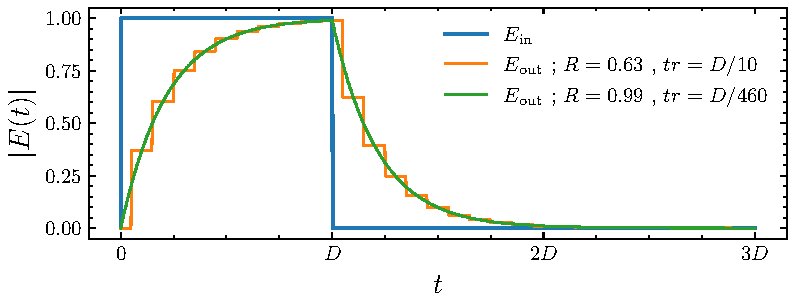
\includegraphics[width=0.7\linewidth]{diagrams/cav_pulse}
	\caption{Plots of (\ref{crds_finite_pulse_onRes}), the output response of an optical cavity to a finite monochromatic pulse which has optical frequency which is tuned to a maximum of the steady state response (\ref{cav_airy}). The magnitude of the electric field incident to the cavity is shown in blue, while two different cavity responses are shown in orange and green. The two responses correspond to a long cavity with low reflectivity and a short cavity with high reflectivity, both keeping the ratio $L/(1-R)$ the same. For the long cavity, the steps are due to the long propagation delay between the mirrors. For cavities of practical length, the green trace is more representative.}
	\label{fig:cavpulse}
\end{figure}

\subsubsection{Off Resonance}

For a monochromatic pulse having optical frequency which does not perfectly match one of the cavity modes, we must use the more general equation (\ref{crds_finite_pulse_general}) for the output field. Using parameters for $t_r$ and $R$ corresponding to a short cavity having high reflectivity mirrors, the plot of equation (\ref{crds_finite_pulse_general}) is shown in Fig. \ref{fig:cavpulsedetuned} for several optical frequencies detuned away from perfect resonance with the cavity.

From these results, we make three key observations
\begin{itemize}
	\item The rate of buildup
	\item The damped oscillations
	\item The ringdown after the pulse has ended
\end{itemize}

\begin{figure}[H]
	\centering
	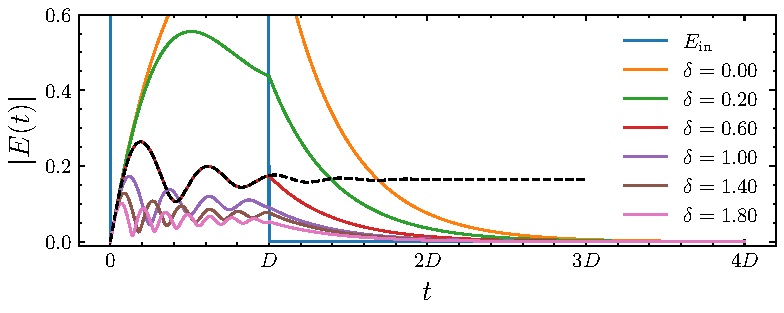
\includegraphics[width=0.7\linewidth]{diagrams/cav_pulse_detuned}
	\caption{Cavity response to a pulsed laser which has wavelength tuned away from the cavity resonance. The electric field amplitude is shown by the blue curve. The detuning from the resonance, $\delta$, gives the frequency of the damped oscillations which occur in the cavity output upon excitation. If the pulse duration $D$ was made long enough, the oscillations would dampen into the constant steady state response given by (\ref{cav_airy}), as shown by the dashed black curve. When the exciting laser is switched off, a clean ringdown transient is observed.}
	\label{fig:cavpulsedetuned}
\end{figure}
It is clear that the maximum buildup rate of the light intensity coming from the cavity corresponds to that which is obtained when the laser and cavity are on resonance (this is the orange trace in Fig. \ref{fig:cavpulsedetuned}). Using the result (\ref{crds_finite_pulse_onRes_approx}) for a short cavity having high reflectivity mirrors, this maximum buildup rate is then
\begin{equation}
	\frac{d\left|E_\mathrm{out}\right|}{dt}\Bigg|_{t=0} = \frac{T}{1-R}\frac{\sqrt{R}}{2\tau_0}
\end{equation}

During the moments when the pulse is switched on, only the first $\theta$ function in (\ref{crds_finite_pulse_general}) is nonzero. We have for the electric field magnitude
\begin{align} \label{cav_pulse_during}
	\left|E_\mathrm{out}\right|^2 &= \frac{T^2}{\left|1-r^2 e^{-i\omega t_r}\right|^2} \left|
	1 - \left(r^2 e^{-i \omega t_r}\right)^{N_1+1}
	\right|^2 \nonumber \\
	&= I_\mathrm{out}(\omega) \;
	\left|
	1 - \left(r^2 e^{-i \omega t_r}\right)^{N_1+1}
	\right|^2
\end{align}
Is is now seen that the output intensity of the cavity approaches the value given by the Airy formula (\ref{cav_airy}) for $I_\mathrm{out}(\omega)$, but with a damped oscillatory factor which determines the transient behavior. In the limit of high reflectivity and short cavity length, the stair-step behavior becomes a continuous one. For this we make the replacement from the discrete $N_1$ to a continuous one $N_1 \rightarrow t/t_r -1/2$.
We then have for the exponential term
\begin{align*}
	q \equiv \left(r^2 e^{-i\omega t_r}\right)^{N_1 +1} &= \left(r^2 e^{-i\omega t_r}\right)^{t/t_r + 1/2} \\
	&= \left(r^2 e^{-i\omega t_r}\right)^{1/2} r^{2t/t_r} e^{-i\omega t}
\end{align*}
We write in terms of the detuning $\delta$ from the cavity resonance frequency $\omega_0$ by introducing $\omega= \omega_0 + \delta$. This gives $r^2 e^{-i\omega_0 t_r} = R$. Using the definition for the reflectivity (\ref{cav_R_defin}) and the exact formula (\ref{tau_vac_exact}) for the ringdown time $\tau_0$ gives $r^{2t/t_r} = e^{-t/2\tau_0} e^{-2i\phi t/t_r}$. Together this gives the result
%	\begin{align*}
	%		q &= \left(r^2 e^{-i\omega t_r}\right)^{1/2} e^{-t/2\tau_0} e^{-2i\phi t/t_r} e^{-i\omega t} \\
	%		&= r e^{-t/2\tau_0} e^{-i\omega t_r/2} e^{-2i\phi t/t_r} e^{-i\omega t} \\
	%		&= \underbrace{\sqrt{R} e^{-t/2\tau_0}}_Q \underbrace{e^{-i\phi}e^{-i\omega t_r/2} e^{-2i\phi t/t_r} e^{-i\omega t}}_{e^{-i\phi'}}
	%	\end{align*}
\begin{align*}
	q &= \left(R e^{-i\delta t_r}\right)^{1/2} e^{-t/2\tau_0} e^{-2i\phi t/t_r} e^{-i\delta t} \cancel{e^{-i \omega_0 t}} \\
	&= \underbrace{\sqrt{R} e^{-t/2\tau_0}}_Q \underbrace{e^{-i\delta t_r/2} e^{-2i\phi t/t_r} e^{-i\delta t}}_{e^{-i\phi'}}
\end{align*}
In the second to last line we have removed the term oscillating at $\omega_0$, the optical frequency of the cavity resonance, since the photodetector will not respond to these oscillations. Above we have defined $Q$ and $\phi'$, the magnitude and phase of the quantity $q$, which allow us to write the term on the right of (\ref{cav_pulse_during}) in the simplified notation
\begin{align*}
	\left|E_\mathrm{out}\right|^2 \propto
	\left|1-q\right|^2 = (1-q^*)(1-q) &= 1 + \left|q\right|^2 - 2\Re \left[q\right] \\
	&= 1 + \left|Q\right|^2 - 2\left|Q\right|\cos\phi'
\end{align*}
We can now evaluate (\ref{cav_pulse_during}) in the limit where the pulse duration is much longer than the cavity round trip time, giving the photodetector response during the pulse as the step response
\begin{equation}\label{cav_pulse_analytic}
	\left|E_\mathrm{out}\right|^2 = I_\mathrm{out}(\omega) \left\{1 + R e^{-t/\tau_0} - 2 \sqrt{R} e^{-t/2\tau_0} \cos\left[\left(\delta + \frac{2\phi}{t_r}\right)t + \frac{\delta t_r}{2}\right]\right\}
\end{equation}
We can now see that the transient behavior is governed by a term decaying with a time constant equivalent to the ringdown time, and an oscillatory term which decays with a time constant which is twice the ringdown time. This behavior is reflected in the plots of Fig. \ref{fig:cavpulsedetuned}, where the square root of the above expression is plotted with the dashed black curve, seen to trace on top of the numerical evaluation of (\ref{crds_finite_pulse_general}).

After the pulse is switched off, there is a contribution from both $\theta$ functions in (\ref{crds_finite_pulse_general}). The electric field squared magnitude is
\begin{align}
	\left|E_\mathrm{out}\right|^2
	%&= \frac{T^2}{\left|1-r^2 e^{-i\omega t_r}\right|^2} \left|
	%\left(r^2 e^{-i \omega t_r}\right)^{N_2+1} - 
	%\left(r^2 e^{-i \omega t_r}\right)^{N_1+1}
	%\right|^2 \nonumber \\
	&=I_\mathrm{out}(\omega) \left|
	\left(r^2 e^{-i \omega t_r}\right)^{N_2+1} - 
	\left(r^2 e^{-i \omega t_r}\right)^{N_1+1}
	\right|^2
\end{align}
Again we get the Airy function for the steady state cavity transmission (\ref{cav_airy}), but modulated with an additional factor. We re-write this factor in a form which makes clear the exponential decay observed in Fig. \ref{fig:cavpulsedetuned} after the driving pulse is turned off. Similar to before, we define the factors
\begin{align*}
	q_1 &\equiv \left(r^2 e^{-i\omega t_r}\right)^{N_1 +1} = \underbrace{\sqrt{R} e^{-t/2\tau_0}}_{Q_1} \underbrace{e^{-i\phi}e^{-i\omega t_r/2} e^{-2i\phi t/t_r} e^{-i\omega t}}_{e^{-i\phi_1'}} \\
	q_2 &\equiv \left(r^2 e^{-i\omega t_r}\right)^{N_2 +1} = \underbrace{\sqrt{R} e^{-(t-D)/2\tau_0}}_{Q_2} \underbrace{e^{-i\phi}e^{-i\omega t_r/2} e^{-2i\phi (t-D)/t_r} e^{-i\omega (t-D)}}_{e^{-i\phi_2'}}
\end{align*}
We use this notational simplification to evaluate the magnitude squared difference appearing in the above expression for $\left|E_\mathrm{out}\right|^2$
\begin{align*}
	\left|E_\mathrm{out}\right|^2 \propto
	\left|q_2 - q_1\right|^2 &= (q_2^* - q_1^*)(q_2 - q_1) = \left|q_2\right|^2 + \left|q_1\right|^2 - 2 \Re\left[q_2^* q_1\right] \\
	&= Q_2^2 + Q_1^2 - 2 Q_1Q_2 \cos\left[\phi_1 - \phi_2\right] \\
	%&= Re^{-t/\tau_0}(1 + e^{D/\tau_0})
	&= R e^{-(t-D)/\tau_0} + R e^{-t/\tau_0} - 2 R e^{-t/\tau_0}e^{D/2\tau_0}\cos\left[2\phi D/t_r +\omega D\right] \\
	%&= R\left\{
	%e^{D/\tau_0} + 1 - 2 e^{D/2\tau_0}\cos\left[2\phi D/t_r +\omega D\right]
	%\right\} e^{-t/\tau_0} \\
	&= R \left\{1 +
	e^{-D/\tau_0} - 2 e^{-D/2\tau_0} \cos\left[2\phi D/t_r +\omega D\right]
	\right\}e^{-(t-D)/\tau_0}
\end{align*}

We see from the above result that after the laser is shut off at time $t=D$, we get a photodetector signal proportional to
\begin{equation}
	\left|E_\mathrm{out}\right|^2 = A e^{-(t-D)/\tau_0}
\end{equation}
This important result highlights that, independent of the laser detuning used to excite the cavity resonance, a clean exponential decay is observed when the input field is completely extinguished. It was seen from expression \ref{cav_pulse_analytic} that oscillating terms appear in the cavity output when the light source is still switched on, complicating the determination of the cavity ringdown time.

This is precisely the motivation for the use of an external modulator for the rapid shutoff of the laser \cite{cw_crds_ROMANINI} when resonance between the laser and cavity is achieved. In this work we employ the use of an acousto-optic modulator (AOM), which can easily achieve sub-100ns shutoff times in the first-order deflected output, as well as extremely large extinction ratios.

\subsection{Sweep of the Laser Across the Cavity Resonance} \label{sec:cav_laser_sweep}
For a high finesse cavity, the overlap of any one of the narrow resonances with the narrow laser line has low probability for occurring at random. Mechanical vibrations result in small jitters of the cavity length which cause a subsequent variation of the FSR. The optical frequency $\nu$ of any one resonance is determined from (\ref{cav_resonance_condition}) as $\nu \approx m\mathrm{FSR}$, where the mode number $m\approx2L/\lambda$ is generally large. The jitter of any one mode position is amplified by a factor which grows with the cavity length. Combined with jitter in the laser wavelength, resonance is difficult to maintain for any extended period of time without active locking. Such an active locking scheme is explored in Sec. \ref{sec:pdh_ringdown}.

A simple method for reliably obtaining short periods of laser-cavity resonance is two sweep either the laser frequency by at least one FSR, or by scanning the cavity length one-half of the laser wavelength. This exploits the repeating mode structure of the cavity by always scanning a size greater than this period. In this section, we make numerical and analytical predictions of a cavity which has a swept laser as input.

We consider here the case of a laser with controllable wavelength which can continuously sweep the across the resonance of an optical cavity. Such a configuration can be used to track the wavelength of the scanning laser, and this was the case for our work on the precision measurement of the xenon hyperfine structure \cite{ours_xe_paper}. As the scan rate is increased, the effect of a finite ringdown time becomes apparent in the signal and can be used to conduct cavity ringdown spectroscopy \cite{crds_rapidSweep_Debecker_05}.

We consider the case of an input field which has a linearly varying instantaneous frequency
\begin{equation}
	E_\mathrm{in}(t) = e^{-i\left[\omega_0 + \frac{1}{2}a t\right]t}
\end{equation}
The derivative of the complex phase gives the instantaneous frequency as $\omega(t) = \omega_0 + a t$. The constant $a$ is the scan rate of the laser in $\mathrm{rad}/\mathrm{s}/\mathrm{s}$.

Plots of the cavity output response (\ref{cav_output_field}) for this particular input field are shown in Fig. \ref{fig:cavsweeps}. For a slow sweep, the output exactly mimics equation (\ref{cav_airy}) for the steady state response. As the sweep rate is increased, the effects of the finite response time of the cavity become apparent as the response becomes shifted, distorted, and diminished. This effect is exaggerated for a high finesse cavity, which is shown in the far-right viewgraph of Fig. \ref{fig:cavsweeps}. Even though the laser spends very little time having its instantaneous frequency resonant with the cavity, the cavity has appreciable output on a time scale comparable to the ringdown time. 

\begin{figure}[H]
	\centering
	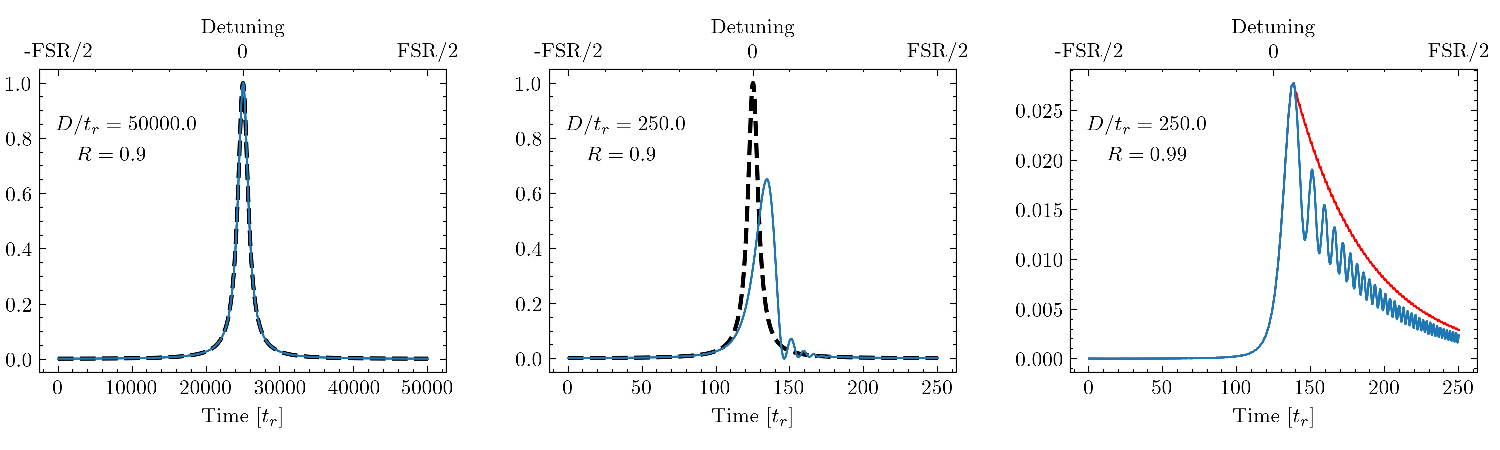
\includegraphics[width=1.0\linewidth]{diagrams/cav_sweeps}
	\caption{Shown is the output of a stationary cavity having its input laser swept in wavelength. Two scanning speeds (proportional to $D/t_r$) are shown; the left graph shows a very slow laser scan accross the resonance, and the middle and right graphs have an increased scanning speed. The cavity finesse is increased from the middle graph to the right graph. For a slow scan across the resonance of low-finesse cavity, the steady state response given by (\ref{cav_airy}), shown with the dashed black plot, is approximately traced out. As the scan speed is increased, the distortion of the transient signal away from the steady state response becomes apparent. Increasing the cavity finesse for a fixed scan speed exaggerates this effect even further, as seen on the rightmost plot. The red curve shown on the right is the effect of turning off the input laser excitation at the output peak, giving a clean ringdown transient. It can be seen that for the rapidly swept case, the rough profile follows this exponential decay.}
	\label{fig:cavsweeps}
\end{figure}

In the right-most viewgraph of the above figure, we consider the rapid sweep of a laser wavelength through a the resonance of a high finesse cavity. The resonance for this cavity is $\sim$10x narrower than for the other cavities shown, and is apparent that the peak response occurs well after the laser has detuned off resonance. Shown also in this right-most viewgraph in red is the response of the cavity if the laser had been instantaneously shut off at the moment of this peak response. It is therefore clear that destructive interference with the input light is the cause of departure from a clean exponential decay. Again, we see the efficacy of using an external modulator to shut off the laser in a time which is small compared to the round trip time of the cavity $t_r$.

\subsubsection{Integral of the Swept Output}
Direct determination of the ringdown time $\tau_0$ of a cavity requires that the transmitted light be detected on sub-microsecond time scale. For a detector which operates much more slowly than this, the output will be proportional to the integral of a single resonance event. That is, we seek a relation of $\int \left|E_\mathrm{out}(t)\right|^2 dt$ for the swept laser input field, integrated over a resonance event.

The time-domain response of the cavity is given by (\ref{cav_output_field}), which gives for the above input field
\begin{align}
	E_\mathrm{out}(t) &= T\sum_{m=0}^{\infty}r^{2m}\exp\left\{-i\omega_0\left(t - \frac{t_r}{2} - mt_r\right)\right\} \exp\left\{ -i\frac{a}{2}\left(t - \frac{t_r}{2} - mt_r\right)^2\right\} \\
	&= e^{-i\omega_0\left(t - t_r/2\right)}e^{-i\frac{a}{2}\left(t - t_r/2\right)^2} T \sum_{m=0}^{\infty}R^{m}e^{i\omega_0 mt_r - i\frac{a}{2}\left(mt_r\right)^2 + iamt_r (t-t_r/2) - 2im\phi} 
\end{align}
We have a sum of the form $S\equiv \sum_{m=0}^{\infty}R^m e^{-i\alpha\left(m^2 - \beta m\right)}$, with the following definitions
\begin{eqnarray}
	\alpha \equiv \frac{at_r^2}{2} &\qquad& \beta \equiv \frac{2\omega_0}{at_r}+ \frac{2}{t_r}\left(t - \frac{t_r}{2}\right) - \frac{4\phi}{at_r^2}
\end{eqnarray}
We can complete the square for the term in the exponential argument \newline $-i\alpha\left[m^2 - \beta m\right] =  -i \alpha \left[\left(m-\frac{\beta}{2}\right)^2 - \frac{\beta^2}{4}\right]$ which allows us to write the sum as
\begin{align*}
	S &= e^{i\alpha \beta^2/4} \sum_{m=0}^{\infty}R^m e^{-i\alpha (m-\beta/2)^2}
\end{align*}

The photodetector response is proportional to the magnitude squared of the cavity output field. The many complex exponential factors appearing in front of the field expression are canceled under this operation, leaving
\begin{align*}
	\left|E_\mathrm{out}(t)\right|^2 &= T^2\left(\sum_{m=0}^{\infty} R^m e^{-i\alpha (m-\beta/2)^2}\right)\left(\sum_{n=0}^{\infty} R^n e^{i\alpha (n-\beta/2)^2}\right) \\
	&= T^2\sum_{m=0}^{\infty}R^{2m} + 2T^2 \sum_{m=0}^{\infty}\sum_{n=m+1}^{\infty}\Re \left\{R^{m+n} e^{i\alpha\left[(m-\beta/2)^2 - (n-\beta/2)^2\right]}\right\} \\
	%&= T^2\sum_{m=0}^{\infty}R^{2m} + 2T^2 \sum_{m=0}^{\infty}\sum_{n=m+1}^{\infty}R^{2m}\cos \left\{\alpha\left[(m-\beta/2)^2 - (n-\beta/2)^2\right]\right\} \\
	&= T^2\sum_{m=0}^{\infty}R^{2m} + 2T^2 \sum_{m=0}^{\infty}\sum_{n=m+1}^{\infty}R^{m+n}\cos \left\{\alpha\left[m^2 - n^2 + (n-m)\beta\right]\right\} \\
	&= \frac{T^2}{1-R^2} + 2T^2 \sum_{m=0}^{\infty}\sum_{n=m+1}^{\infty}R^{m+n}\cos \Bigg\{\frac{at_r^2}{2}\left[m^2 - n^2 + (n-m)\left(\frac{2t}{t_r} - 1\right)\right] \nonumber\\
	&\qquad\qquad\qquad\qquad\qquad\qquad\qquad\qquad\qquad
	+ (n-m)\left(\omega_0 t_r - 2\phi\right)\Bigg\}
\end{align*}
The argument to the cosine function in the above nested sum is of the simple form
\begin{equation*}
	\cos\left[(n-m) a t t_r + \Phi(n,m,t_r,\omega_0)\right]
\end{equation*}
If we set the scanning rate such that one free spectral range is scanned in a time $D$, we have $a=2\pi/t_rD$. We can guarantee that each of the cosine terms in the above nested sum integrates to zero by choosing the integration time from $0$ to $D$. This trivially gives the integral of the photodetector signal of the cavity output for the swept laser as
\begin{equation}
	\int_{0}^{D}\left|E_\mathrm{out}(t)\right|^2 dt = \frac{DT^2}{1-R^2} \simeq \frac{T^2 D}{t_r}\tau_0
\end{equation}

We now come to the conclusion that the integral of the cavity output light is proportional to the ringdown time of the cavity $\tau_0$. For a slow detector, this observation allows us to determine the ratio of two ringdown times $\tau/\tau_0$. In general, direct determination of the ringdown time from such an expression is tricky since we must resolve the proportionality constant, which includes the detector gain. It is much easier to measure two such events, keeping the proportionality constant the same, and take the ratio. This is the principle by which absorption is computed in some instances of Vernier spectroscopy, especially those where a slow focal plane array detector is used.

The proportionality to $\tau_0$ is most easily seen from the simple case of a clean exponential decay emerging from the cavity
\begin{equation*}
	\int_{0}^{\infty} A e^{-t/\tau_0} = A\tau_0
\end{equation*}

\subsection{Sweep of the Cavity Resonance Across the Laser}
Here we consider the case of a linear cavity having its round trip length changed as a function of time. This corresponds to the realistic case of a cavity having a piezo electric actuator attached to one of the mirrors, allowing a slight modulation of the cavity length $L\rightarrow L(t)$. For now we consider the case of a cavity mirror moving at a constant velocity, giving the time dependent length
\begin{equation}
	L(t) = L_0 + vt
\end{equation}

We cannot use equation (\ref{cav_output_field}) as before. Return to the construction of Fig. \ref{fig:cavitytransmission}, the cavity output field in response to monochromatic input $E_\mathrm{in}(t) = E_0 e^{-i\omega t}$ is then \cite{crds_ultraslow_velocities, Gohle_Dissertation_2006}
\begin{equation}
	E(t) = E_0 t^2 \sum_{n=0}^{\infty}r^{2m}\exp\left\{i\frac{\omega}{c}\left[L + 2\sum_{m=1}^{n}L(t_m)\right] - i\omega t\right\}
\end{equation}

\begin{equation}
	t_m = t - \frac{(2m-1)L_0}{c}
\end{equation}

%In order to compute the response of this length-modulated optical cavity to an arbitrary input field, we must upgrade expression (\ref{cav_output_field}) to include the changing delay of the cavity. We remind the reader that expression (\ref{cav_output_field}) can be directly obtained by the construction of Fig. \ref{fig:cavitytransmission}, and we can perform the upgrade of this expression using the same construction. Denoting the complex transmission coefficient as $\tilde{t}$ to avoid confusion with time, the beamlets in Fig. \ref{fig:cavitytransmission}(b) have the time-dependent delay

For $v/c<<1$, the sum in the exponent can be evaluated
\begin{align}
	\sum_{m=1}^{n}L(t_m) &= \sum_{m=1}^{n}\left(L_0 + v t_m\right) \\
	&= n\left[\left(1-n\frac{v}{c}\right)L_0 + vt\right] \\
	&= nc\left[(1-n\beta)\frac{t_r}{2} + \beta t\right]
\end{align}

This gives the cavity output as
\begin{equation}
	E(t) = E_0 e^{i(\omega L_0/c - \omega t)}\sum_{n=0}^{\infty}r^{2n}\exp\left\{i2n\omega\left[(1-n\beta)\frac{t_r}{2} + \beta t\right]\right\}
\end{equation}

We can see that when illuminated with light of a single frequency $\omega$, the cavity output features many additional frequencies. This non-linearity of the output means that we cannot represent the swept cavity output by a simple transfer function. This can be intuitively understood by the doppler shift of the light which is reflected from the moving mirror. Upon each reflection, the light experiences a doppler shift of its frequency. After many reflections in the cavity, the many doppler shifts of the beam give a mixture of frequencies which were not originally present in the beam.

\subsection{Time Domain Signal of CRDS} \label{sec:cav_crds}

In this section we attempt to model a realistic transient of a cavity resonance swept across a laser line, with the laser light being shut off during the excitation. Such a configuration is common for CRDS, where a swept cavity is used to guarantee a resonance condition with laser light of arbitrary wavelength, and an external modulator to rapidly extinguish the incident light in the middle of the excitation.

Plotted in Fig. \ref{fig:crds_aomsimulation} is the ratio $\left|E_\mathrm{out}\right|/\left|E_\mathrm{in}\right|$ for two different cavities, on the left having $R=0.99$ and on the right $R=0.998$, and both cavities are swept at identical rates. Overlayed on both plots is the result of shutting off the exciting laser at different times.

\begin{figure}[H]
	\centering
	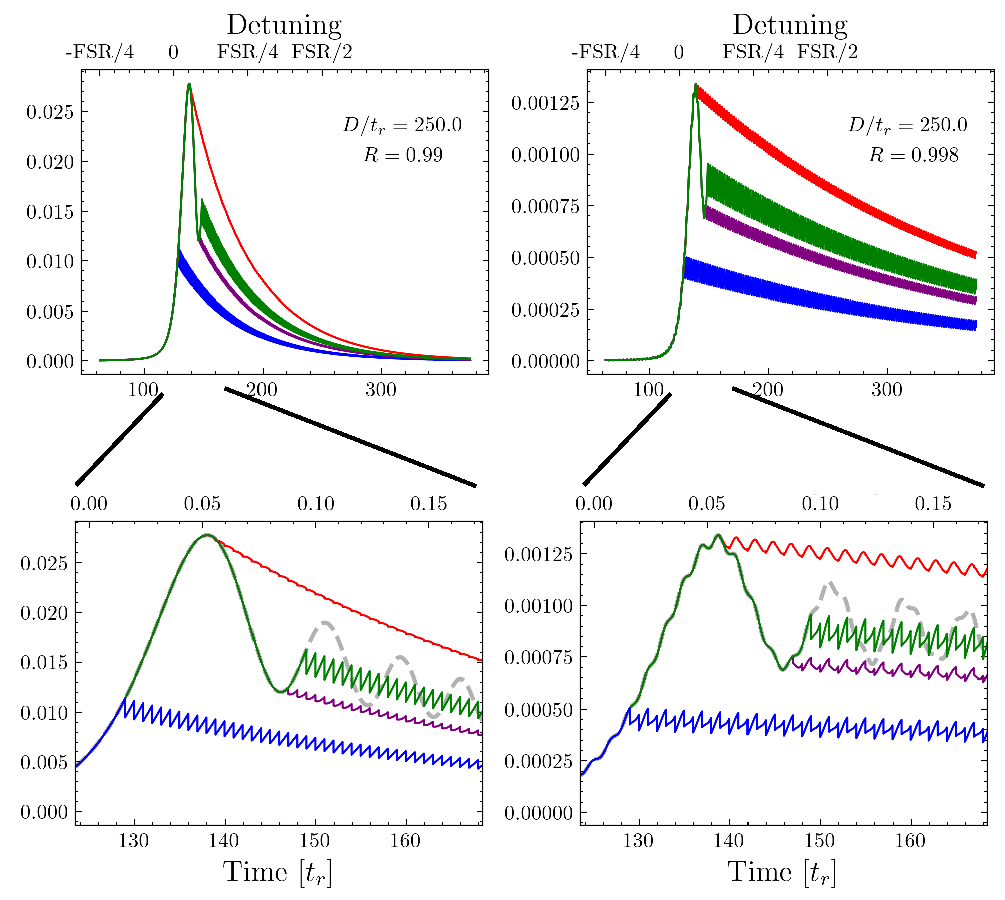
\includegraphics[width=0.7\linewidth]{diagrams/crds_AOMsimulation}
	\caption{Simulated output of a cavity with scanning length having a laser with stationary wavelength mode-matched to the input. The black dashed curve shows the transient response of the cavity for a laser that is always on. The colored curves correspond to different places in the transient where the exciting laser is switched off. It can be seen that the effect of switching off the laser near the onset of resonance is to give a curve which decays exponentially and is superimposed with harmonics of the cavity FSR. For a high-finesse cavity, these harmonics are easily filtered from the cavity transient by electronic filters. It can also be seen that the effect of switching off the laser is to eliminate lower frequency beating behavior which is much more difficult to eliminate. It is therefore almost always preferable to use an external modulator to eliminate these effects from CW ringdown measurements.}
	\label{fig:crds_aomsimulation}
\end{figure}

It can be seen that after the exciting laser is shut off, the signal follows an exponential decay which has a $1/e$ constant of $\tau$ the cavity ringdown time. This exponential decay is accompanied by high frequency beating having frequencies which are harmonics of the cavity FSR, a fact which is established by the fact that the beating is periodic with period $t_r = 1/\mathrm{FSR}$. It can be seen from Fig. \ref{fig:crds_aomsimulation} that the amplitude of the beating signal is dependent on the part of the exitation curve where the laser is shut off, having minimum amplitude when the shutoff time corresponds to a critical point of the output light.

From our previous discussion, we may surmise that the post-shutoff CRDS signal has the form
\begin{equation}
	I(t) = A e^{-t/\tau} + B(t) e^{-t/2\tau}
\end{equation}

The beating terms are described by a function $B(t)$ which is periodic with period $t_r$, the round-trip time of the cavity. If the ringdown time $\tau$ of the cavity is much longer than the cavity round-trip time, these beating signals may be effectively filtered out by a lowpass filter. Performing this filtering of the beating signals removes the requirement that the digital acquisition system operate at a sampling rate which is multiple times the FSR of the cavity, otherwise these high frequency beat signals will be aliased into ripples. By filtering the high frequency beat notes, the acquisition system can then be optimized for the measurement of a clean exponential signal

\begin{equation}
	I_\mathrm{filtered}(t) = A e^{-t/\tau} + O
\end{equation}

In the above expression $O$ represents a residual offset from the filtering process. In practice, this term can encompass other experimental factors such as offsets from photodetector amplifiers and the calibration of the voltage offset of the acquisition system. The above expression serves as a sufficient fitting model for experimental measurements of decaying post-shutoff light emerging from an excited optical cavity, and it is this model that we will use for fitting ringdown curves in this dissertation.

\section{Experimental Realization of Cavity Properties}
In this section we demonstrate experimentally some of the theoretical results of the previous section. These will be focused on methods of resolving the cavity mode structure, which aids in the alignment of the input beam, and the measurement of the cavity ringdown time, which is important for sensitive spectroscopic measurements.

\subsection{Higher Order Mode Structure} \label{sec:cav_alignment}
When aligning a laser beam to an optical cavity, the coupling is very sensitive to the propagation direction of the beam even when the transverse profile is perfectly mode matched to the cavity (Sec. \ref{sec:mode-matching}). An exception is made for the confocal cavity, which has the greatest acceptance of the input beam \cite{book_lasers_siegman}.

A slightly misaligned beam will cause excitation of higher order modes spatial modes in the cavity, and these can be detected in the transmission of the cavity. We can optimize the laser-cavity coupling by minimizing the excitation of these higher order cavity modes and maximizing the excitation of the fundamental mode. The relative excitation of the higher order modes may be realized using the fact that the higher order modes generally have a different resonance frequency than the fundamental modes. For a Hermite-Gauss mode having indices $m$ and $n$, there is an additional Guoy phase shift which shifts the location of the resonance. For a cavity having round trip length $\ell$, the round trip phase shift must be a multiple of $2\pi$, so the modes higher order modes must satisfy \cite{book_lasers_siegman}
\begin{equation}
	\frac{\omega \ell}{2c} - \left(n + m + 1\right)\cos^{-1}\pm \sqrt{g_1 g_2} = q \pi
\end{equation}
where $q$ is an integer. The $g_{1,2}$ parameters were defined in Sec. \ref{sec:cav_ABCD} as the dimensionless parameters defining the cavity geometry. In terms of these parameters, the resonance frequencies are then given by
\begin{equation} \label{cav_higherOrder_mode_freqs}
	\nu_{qmn} = \left[q + (n + m + 1) \frac{\cos^{-1}\pm\sqrt{g_1 g_2}}{\pi}\right] \frac{c}{\ell}
\end{equation}
The factor $\cos^{-1}\pm\sqrt{g_1 g_2}/\pi$ is bounded by $\pm 1$, so the higher order modes generally appear between the axial resonances, here enumerated by $q$. For the linear cavity shown in Fig. \ref{fig:cavitymodematch} we have $g_1 = 1$ (corresponding to the flat mirror). The cavity dimensions $L=1.72m$ and $R=2m$, give $g_2 \approx 0.14$. The higher order modes are located at a fraction $\cos^{-1}\pm\sqrt{g_1 g_2}/\pi \approx 0.38$ of the free spectral range.

Using a laser of fixed wavelength, we can scan these resonances by slightly modulating the cavity length using a piezoelectric actuator attached to one of the cavity mirrors. As the length of the cavity is scanned different modes come into resonance with the laser. If the scan amplitude is large enough, a repeating pattern of resonances will be observed corresponding to the free spectral range of the cavity. In Fig. \ref{fig:cavalignmentmodes}, we show such a scan of a cavity in a misaligned condition, where a higher order mode is seen at roughly one-third of the scan of the free spectral range, in agreement with our calculation for this cavity. The same cavity is shown after adjusting the cavity alignment to suppress the excitation of this higher order mode.

\begin{figure}[H]
	\centering
	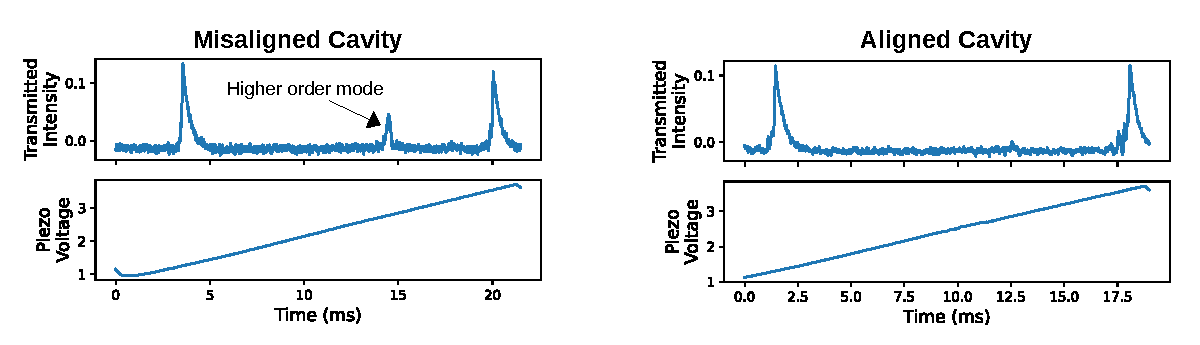
\includegraphics[width=1.0\linewidth]{diagrams/cav_alignmentModes}
	\caption{The final alignment of an optical cavity can be performed by observing the transmitted mode structure when the cavity length is scanned by changing the voltage applied to a piezoelectric actuator. In both graphs, the spacing between the large transmitted peaks represents the free spectral range of the cavity. Appearing on the left graph between these larger peaks is a smaller peak which is evidence of a transmitted higher mode. By adjusting the laser-cavity alignment, the graph on the right is obtained where the higher-order mode excitation is nearly extinguished. The relative spacing of the higher order modes compared to the FSR are given by (\ref{cav_higherOrder_mode_freqs}).}
	\label{fig:cavalignmentmodes}
\end{figure}

Critical to this alignment is the ability to recognize the repeating pattern of modes corresponding to a complete scan of one free spectral range. This task can be slightly complicated when the location of the higher order modes form evenly spaced locations. In the linear cavity example, the higher order modes form at appoximately 1/3 the free spectral range spacing. When the cavity is severly misaligned, we see the presence of the next higher order mode at 2/3 of the FSR spacing which gives the impression that the repeating pattern is three times smaller than it actually is.

\subsection{On-Resonant Behavior of the Cavity Output} \label{sec:pdh_ringdown}
In sec. \ref{sec:cav_td_response}, we showed that the cavity has a simple filtering behavior for intensity fluctuations of on-resonant monochromatic input light. The characteristic time of this filtering gives a measure of the cavity ringdown time. In this section we show how a direct measurement of this effect could be conducted in practice, leading to a method which can directly measure the ringdown time of the cavity in the most rapid possible manner.

For a high finesse cavity, it is difficult to ensure overlap of the narrow cavity mode with the laser wavelength. Mechanical vibrations in the optical setup cause jitter in the location of any one cavity resonance, and unless active stabilization methods are used, the laser also experiences jitter in the output wavelength. One such active stabilization technique is the Pound-Drever-Hall technique \cite{PDH_locking} for locking a laser's wavelength to a cavity resonance. This technique can also be modified to instead stabilize the cavity length, where the location of a single cavity resonance is locked to the laser wavelength.

Shown in Fig. \ref{fig:cavpdhlock} is a ring cavity which has been modematched to an input laser beam. The beam profile and modematching condition were shown for this particular cavity in Fig. \ref{fig:cavitymodematch}. The input beam first passes through an electro-optic modulator (EOM) which puts phase modulation sidebands on the optical spectrum of the laser. In the presence of the cavity resonance the sidebands are unbalanced, creating a beat note at the EOM driving frequency which is seen at the reflection photodiode. This signal (shown in orange) is demodulated using a double balance mixer and low pass filter which gives a signal which is approximately the derivative of the resonance signal (shown in yellow). This is used as an error signal since it has a linear zero crossing at the point of resonance. The servo loop uses this error signal to provide correction to the cavity length via the piezo electric actuator which is shown in the diagram as PZT.

We note that this is slightly different than the original conception of the Pound-Drever-Hall technique \cite{PDH_locking}, where the feedback is applied to the cavity instead of the laser. In certain cases this is desirable, since it may be possible that the laser line is more stable than the cavity resonance.

In Fig. \ref{fig:cavpdhlock} we have also shown an AOM, which allows the intensity of the laser beam to be rapidly modulated by changing the amplitude of the driving RF signal. For this laser, the optical power could not be adjusted independently of the wavelength, so the AOM is used to provide a square wave modulation to the optical power input to the cavity. When the cavity is locked to the laser using the PDH technique, we investigate the cavity response to a square wave modulated input.


\begin{figure}[H]
	\centering
	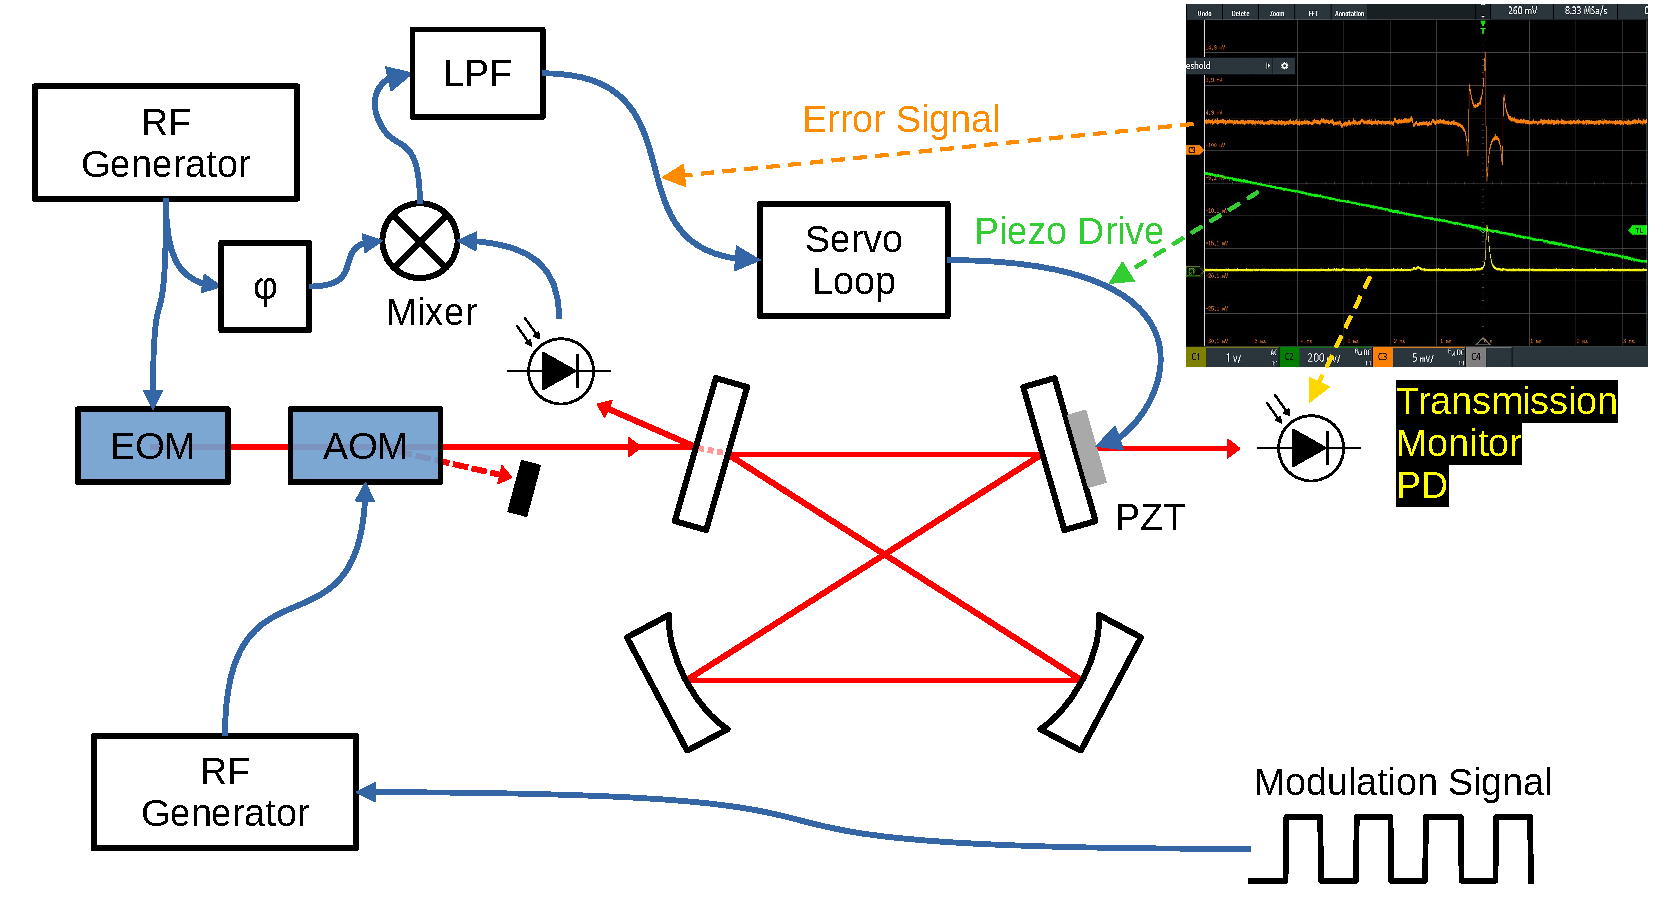
\includegraphics[width=0.7\linewidth]{diagrams/cav_pdhLock}
	\caption{A setup for the stabilization of an optical cavity length to ensure that the laser and cavity are always on resonance. Stabilization is performed using the Pound-Drever-Hall technique, and feedback is performed on a piezoelectric actuator (PZT) attached to one of the cavity mirrors. By modulating the power of the input laser beam, the ringdown time is extracted by the filtering action of the cavity on the output light. This scheme represents the fastest possible ringdown time measurement method, being limited only by the duration of the ringdown transient itself.}
	\label{fig:cavpdhlock}
\end{figure}

It can be seen from the results in Fig. \ref{fig:cavpdhlockoutput} that the cavity response to a square-wave modulated input has the same behavior that was found from the theoretical analysis in the previous section. In fact, the response is well modeled by the equation (\ref{crds_finite_pulse_onRes_approx}), which means that the ringdown time can be extracted by fitting the response.

\begin{figure}[H]
	\centering
	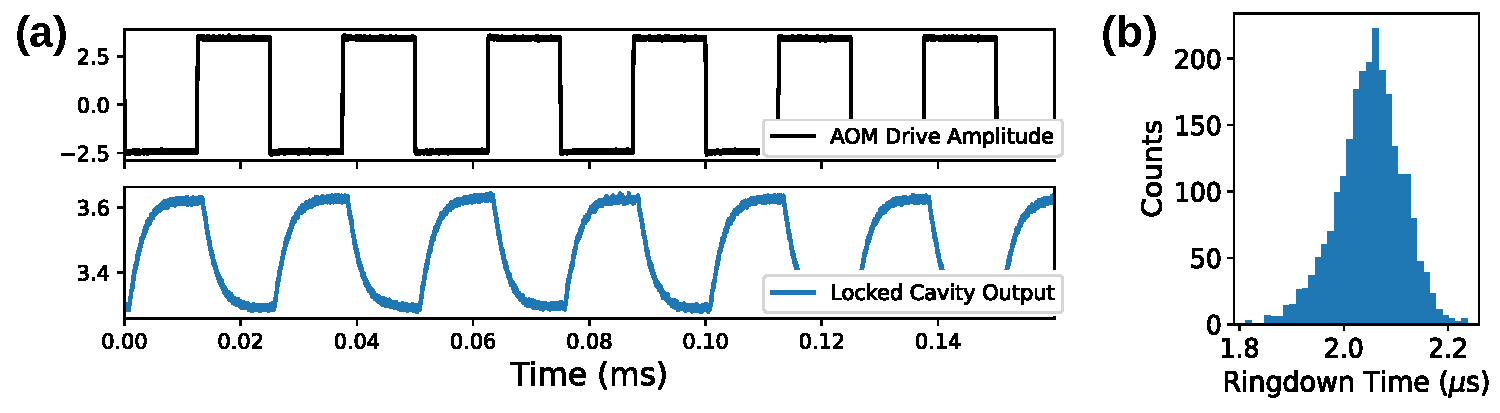
\includegraphics[width=0.8\linewidth]{diagrams/cav_pdhLock_output}
	\caption{Response of the locked cavity to the intensity modulated input light. The black trace shown in \textbf{(a)} is the trigger signal which enables and disables the RF drive for the AOM. This causes the light input light, having its wavelength locked to the cavity resonance, to be intensity modulated due to some of the light being deflected into the first order output of the AOM. The lower blue trace is the response of the cavity to the on-resonant intensity modulated light. The resemblance to the theoretical response shown in Fig. \ref{fig:cavpulse} is clear. Shown in \textbf{(b)} is the result of fitting many of the transitions to extract the ringdown time. The acquisition rate of 4kHz shown here is essentially the fastest possible for this cavity, as shortening the observation duration negatively impacts the retrieved fits.}
	\label{fig:cavpdhlockoutput}
\end{figure}

The proof-of-concept setup presented here illustrates the fastest possible acquisition scheme for ringdown transients. Since the laser is always on resonance with the cavity, no time is spent waiting for the laser or cavity to scan onto resonance with one another. Even in this tightly locked scheme, we are ultimately limited by the length of the ringdown transient itself. If for accurate fitting, we require $\sim 5\tau$, then the maximum possible acquisition rate is $1/5\tau$.

%	\subsection{Off-Resonant Behavior of the Cavity Output}
%	\begin{itemize}
	%		\item \textbf{\hl{Show the CRDS-style "sweep onto resonance" configuration in its simplest form.}}
	%		\item \textbf{\hl{Emphasis on the hardware simplification this brings.}}
	%	\end{itemize}